\documentclass[12pt,a4paper]{article}
\usepackage[utf8]{inputenc}
\usepackage[T5]{fontenc}
\usepackage[vietnamese]{babel}
\usepackage{mathptmx}           % Times New Roman font
\usepackage{geometry}
\geometry{top=2cm, bottom=2cm, left=2.5cm, right=2cm, headheight=14.5pt}
\usepackage{longtable}
\usepackage{array}
\usepackage{amssymb}
\usepackage{indentfirst}
\usepackage{booktabs}
\usepackage{xcolor}
\usepackage{colortbl}
\usepackage{enumitem}
\usepackage{graphicx}
\usepackage{float}
\usepackage{fancyhdr}
\usepackage{lastpage}
\usepackage{tikz}
\usetikzlibrary{calc}

% --- Cấu hình đường dẫn ảnh ---
\graphicspath{{../images/}}

\definecolor{headerblue}{RGB}{220,230,242}
\definecolor{notegreen}{RGB}{234,250,234}

% --- Cấu hình Header & Footer ---
\pagestyle{fancy}
\fancyhf{}
\fancyhead[L]{\small \leftmark}
\fancyhead[R]{\small Trang \thepage/\pageref{LastPage}}
\renewcommand{\headrulewidth}{0.4pt}
\renewcommand{\sectionmark}[1]{\markboth{#1}{}}
\setcounter{tocdepth}{3}
\setcounter{secnumdepth}{3}

\begin{document}

\begin{titlepage}
    \newgeometry{left=2cm, right=2cm, top=2cm, bottom=2cm}
    \begin{tikzpicture}[remember picture, overlay]
        \draw[line width = 2pt] ($(current page.north west) + (1.5cm,-1.5cm)$) rectangle ($(current page.south east) + (-1.5cm,1.5cm)$);
        \draw[line width = 0.5pt] ($(current page.north west) + (1.6cm,-1.6cm)$) rectangle ($(current page.south east) + (-1.6cm,1.6cm)$);
    \end{tikzpicture}

    \begin{center}
        \large \textbf{HỌC VIỆN CÔNG NGHỆ BƯU CHÍNH VIỄN THÔNG} \\
        \large \textbf{KHOA CÔNG NGHỆ THÔNG TIN 2} \\
        \large \textbf{BỘ MÔN THỰC TẬP CƠ SỞ} \\
        \vspace{0.5cm}
        \rule{3cm}{1pt} \\

        \vspace{1.2cm}
        
\includegraphics[width=5.5cm]{Logo_PTIT_University.png} \\
        \vspace{1.5cm}

        \LARGE \textbf{BÁO CÁO CUỐI KỲ} \\
        \vspace{0.5cm}
        \Large \textbf{PHÂN TÍCH VÀ XÁC ĐỊNH YÊU CẦU HỆ THỐNG} \\
        \vspace{1cm}

        \begin{minipage}{14cm}
            \centering
            \large \textbf{Đề tài: Hệ thống nhận diện bệnh trên cây lúa dựa trên thuật toán học sâu CNN}
        \end{minipage}

        \vspace{2.5cm}

        \begin{tabular}{l l}
            \textbf{Giảng viên hướng dẫn:} & Cô Nguyễn Thị Bích Nguyên           \\
            \textbf{Nhóm:}                 & Nhóm 1                              \\
            \textbf{Lớp:}                  & E23CQCE01-N                         \\
            \textbf{Sinh viên thực hiện:}  & 1. Phan Tuấn Quốc Anh - N23DCCN003  \\
                                           & 2. Phạm Minh Khang - N23DCAT034     \\
                                           & 3. Nguyễn Lê Minh Phúc - N23DCDK058 \\
        \end{tabular}

        \vfill
        \large \textbf{TP. HỒ CHÍ MINH - 2026}
    \end{center}
    \restoregeometry
\end{titlepage}

\clearpage
\tableofcontents
\clearpage
\listoffigures
\clearpage
\listoftables
\clearpage

% ============================================================
\section{Tầm nhìn dự án}

\begin{longtable}{|l|p{11.5cm}|}
    \caption{Tầm nhìn dự án}                                                                                                                                 \\
    \hline
    \rowcolor{headerblue}
    \textbf{Mục}               & \textbf{Nội dung}                                                                                                           \\
    \hline
    \textbf{Nỗi đau hiện tại}  & Chẩn đoán bệnh trên cây lúa bằng mắt thường dẫn đến kết quả sai lệch, xử lý chậm trễ (1--3 ngày) và lạm dụng thuốc hóa học. \\
    \hline
    \textbf{Giải pháp đề xuất} & Ứng dụng trí tuệ nhân tạo (CNN) nhận diện bệnh qua hình ảnh, kết hợp dữ liệu thời tiết (GPS) và gợi ý dinh dưỡng thực vật.  \\
    \hline
    \textbf{Giá trị mang lại}  & Chẩn đoán nhanh (5--7 giây), chính xác, giảm phụ thuộc thuốc hóa học, nâng cao năng suất nông nghiệp.                       \\
    \hline
    \textbf{Ngoài phạm vi}     & Cảm biến IoT, thương mại điện tử, tích hợp ERP doanh nghiệp.                                                                \\
    \hline
\end{longtable}

% ============================================================
\section{Quy trình hiện tại và quy trình đề xuất}

\textbf{Quy trình hiện tại (As-Is):}
\begin{enumerate}
    \item Nông dân phát hiện triệu chứng bất thường trên lá lúa.
    \item Tự đoán bệnh dựa trên kinh nghiệm hoặc hỏi người xung quanh (mất 1--3 ngày).
    \item Mua thuốc bảo vệ thực vật theo cảm tính, dễ lạm dụng hóa chất.
\end{enumerate}

\textbf{Quy trình đề xuất (To-Be):}
\begin{enumerate}
    \item Nông dân chụp ảnh lá lúa bằng điện thoại.
    \item Hệ thống AI nhận diện bệnh trong 5--7 giây, khoanh vùng bệnh trên ảnh.
    \item Hệ thống gợi ý dinh dưỡng phù hợp với loại bệnh được phát hiện.
    \item Nông dân có thể phản hồi nếu kết quả chưa chính xác.
    \item Dữ liệu phản hồi được dùng để tái huấn luyện và nâng cấp mô hình AI.
\end{enumerate}

\hrulefill

% ============================================================
\section{Phạm vi áp dụng đề tài}
\begin{itemize}
    \item \textbf{Phạm vi nghiệp vụ:} Hệ thống số hóa quy trình chẩn đoán bệnh lúa qua hình ảnh bằng công nghệ nhận diện chuyên sâu. Hệ thống kết hợp phân tích hình ảnh và các thông số môi trường để đưa ra chẩn đoán chính xác. Kết hợp xây dựng kho tri thức về dinh dưỡng thực vật để gợi ý các loại vitamin và vi lượng cần bổ sung dựa trên việc truy xuất dữ liệu thông minh.
    \item \textbf{Phạm vi đối tượng:} Phục vụ Nông dân (nhận diện \& nhận gợi ý dinh dưỡng) và Quản trị viên (quản lý danh mục, cập nhật mô hình, quản lý kho kiến thức hệ thống).
    \item \textbf{Giới hạn đề tài:} Hệ thống tự chủ kho dữ liệu dinh dưỡng nội bộ. Đối với thông số môi trường, hệ thống sử dụng tọa độ vị trí (GPS) để tự động truy xuất dữ liệu thời tiết làm dữ liệu phụ trợ. Hỗ trợ nhận diện nhiều loại bệnh cùng lúc trên cùng một ảnh.
\end{itemize}

% ============================================================
\section{Các bước xác định yêu cầu}

Quá trình thực hiện xác định yêu cầu gồm 2 bước chính như sau:
\begin{itemize}
    \item \textbf{Bước 1:} Khảo sát hiện trạng, kết quả nhận được là các báo cáo về hiện trạng chẩn đoán bệnh trên cây lúa và nhu cầu bổ sung dinh dưỡng.
    \item \textbf{Bước 2:} Lập danh sách các yêu cầu, kết quả nhận được là danh sách các yêu cầu sẽ được thực hiện trên hệ thống máy tính.
\end{itemize}

\subsection{Đối tượng tham gia xác định yêu cầu}
Gồm 2 nhóm người:
\begin{itemize}
    \item \textbf{Chuyên viên tin học:} Thiết kế kiến trúc nhận diện thông minh, xây dựng kho kiến thức hệ thống và luồng xử lý truy xuất thông tin dinh dưỡng chính xác nhất.
    \item \textbf{Nhà chuyên môn (Kỹ sư nông nghiệp):} Cung cấp dữ liệu ảnh kèm thông số môi trường tương ứng, gán nhãn bệnh và trực tiếp biên soạn/chuẩn hóa bộ dữ liệu văn bản về vitamin/dinh dưỡng.
\end{itemize}
Hai nhóm người này phối hợp thật chặt chẽ để có thể xác định đầy đủ và chính xác các yêu cầu.

\hrulefill

\subsection{Khảo sát hiện trạng}
\subsubsection{Các hình thức thực hiện phổ biến}
\begin{itemize}
    \item \textbf{Quan sát:} Theo dõi và ghi hình quá trình cây lúa biểu hiện triệu chứng thiếu hụt dinh dưỡng hoặc mắc nhiều bệnh cùng lúc trên đồng ruộng dưới các điều kiện thời tiết khác nhau.
    \item \textbf{Khảo sát:} Khảo sát các người nông dân về mối liên hệ giữa các loại bệnh lúa, sự thiếu hụt dinh dưỡng và sự tác động của môi trường (nhiệt độ, độ ẩm).
    \item \textbf{Thu thập thông tin, tài liệu:} Thu thập tập dữ liệu ảnh lá lúa (kèm dữ liệu đặc tả về thời tiết/độ ẩm) và chuẩn bị bộ dữ liệu văn bản về dinh dưỡng thực vật.
\end{itemize}

\subsubsection{Quy trình thực hiện}
\textbf{A. Tìm hiểu tổng quan về thế giới thực:}
\begin{itemize}
    \item Quy mô hoạt động nông nghiệp, các bệnh dịch thường gặp.
    \item Xu hướng chuyển dịch sang bổ sung vitamin tăng sức đề kháng thay vì lạm dụng thuốc hóa học.
\end{itemize}

\textbf{B. Tìm hiểu hiện trạng tổ chức (cơ cấu tổ chức):}
\begin{itemize}
    \item Cơ cấu tổ chức bao gồm các chức danh: Quản trị viên (Quản lý dữ liệu bệnh, mô hình, tập dữ liệu dinh dưỡng), Nông dân (tải ảnh và mô tả tình trạng).
\end{itemize}

\textbf{C. Tìm hiểu hiện trạng nghiệp vụ:}
\begin{itemize}
    \item Việc tìm hiểu dựa trên: Thông tin đầu vào, Quá trình xử lý, Thông tin kết xuất.
    \item Xếp loại các nghiệp vụ vào 4 loại: Lưu trữ, Tính toán, Tra cứu, Kết xuất.
\end{itemize}

\hrulefill

\subsection{Lập danh sách các yêu cầu}
\subsubsection{Xác định yêu cầu chức năng nghiệp vụ}

% ============================================================
% NGƯỜI DÙNG: NÔNG DÂN
% ============================================================
\section{Người dùng --- Nông dân (Mã số: ND)}

\textbf{Định nghĩa:} Người sử dụng hệ thống với mục đích chẩn đoán bệnh trên cây lúa qua hình ảnh, xem gợi ý dinh dưỡng và phản hồi kết quả chẩn đoán.

\vspace{0.3cm}
\textbf{1. Bảng yêu cầu chức năng nghiệp vụ}

\begin{longtable}{|
        c|
        >{\raggedright\arraybackslash}p{3.2cm}|
        >{\raggedright\arraybackslash}p{2.2cm}|
        >{\raggedright\arraybackslash}p{2.4cm}|
        >{\raggedright\arraybackslash}p{2.6cm}|
        >{\raggedright\arraybackslash}p{2.6cm}|}
    \hline
    \rowcolor{headerblue}
    \textbf{STT} & \textbf{Công việc}               & \textbf{Loại công việc} & \textbf{Quy định/CT liên quan} & \textbf{Biểu mẫu liên quan} & \textbf{Ghi chú}         \\
    \hline
    \endhead
    \multicolumn{6}{|l|}{\cellcolor{notegreen}\textbf{I. Quản lý tài khoản}}                                                                                            \\
    \hline
    1            & Đăng ký tài khoản                & Lưu trữ                 & QĐ-ND-01                       & ND\_BM 1                    &                          \\
    \hline
    2            & Đăng nhập hệ thống               & Tra cứu                 & QĐ-ND-01                       & ND\_BM 1b                   &                          \\
    \hline
    3            & Khôi phục mật khẩu               & Lưu trữ                 & QĐ-ND-01                       &                             &                          \\
    \hline
    4            & Đổi mật khẩu                     & Lưu trữ                 & QĐ-ND-01                       & ND\_BM 1c                   &                          \\
    \hline
    5            & Đăng xuất hệ thống               & Lưu trữ                 & QĐ-ND-01                       &                             &                          \\
    \hline
    \multicolumn{6}{|l|}{\cellcolor{notegreen}\textbf{II. Hồ sơ cá nhân}}                                                                                               \\
    \hline
    6            & Xem thông tin cá nhân            & Tra cứu                 & QĐ-ND-02                       &                             &                          \\
    \hline
    7            & Chỉnh sửa thông tin cá nhân      & Lưu trữ                 & QĐ-ND-02                       & ND\_BM 2                    &                          \\
    \hline
    \multicolumn{6}{|l|}{\cellcolor{notegreen}\textbf{III. Chẩn đoán bệnh lúa}}                                                                                         \\
    \hline
    8            & Gửi ảnh lúa để chẩn đoán         & Lưu trữ                 & QĐ-ND-03                       & ND\_BM 3                    &                          \\
    \hline
    9            & Nhập thông số môi trường bổ sung & Lưu trữ                 & QĐ-ND-03                       &                             & Tùy chọn, không bắt buộc \\
    \hline
    10           & Xem kết quả chẩn đoán            & Tra cứu, Tính toán      & QĐ-ND-03                       &                             &                          \\
    \hline
    \multicolumn{6}{|l|}{\cellcolor{notegreen}\textbf{IV. Tra cứu \& Phản hồi}}                                                                                         \\
    \hline
    11           & Tra cứu lịch sử chẩn đoán        & Tra cứu                 & QĐ-ND-04                       &                             &                          \\
    \hline
    12           & Xem chi tiết một lần chẩn đoán   & Tra cứu                 & QĐ-ND-04                       &                             &                          \\
    \hline
    13           & Gửi phản hồi kết quả             & Lưu trữ                 & QĐ-ND-05                       & ND\_BM 4                    &                          \\
    \hline
    14           & Xem kết quả xử lý phản hồi       & Tra cứu                 & QĐ-ND-05                       &                             &                          \\
    \hline
\end{longtable}
\vspace{0.3cm}
\noindent\textbf{QĐ-ND-01 --- Quy định Tài khoản}

\noindent\textit{a) Đăng ký tài khoản}

\noindent\textbf{Quy trình đăng ký:}
\begin{enumerate}
    \item Người dùng cung cấp: \textbf{Tên đăng nhập} (duy nhất), \textbf{Email} (duy nhất), \textbf{Mật khẩu} và \textbf{Xác nhận mật khẩu}.
    \item \textbf{Ràng buộc mật khẩu:} Tối thiểu 8 ký tự, bao gồm ít nhất 1 chữ cái viết hoa, 1 chữ số và 1 ký tự đặc biệt.
    \item Hệ thống gửi liên kết xác thực hoặc mã OTP về email để kích hoạt tài khoản.
\end{enumerate}

\noindent\textit{b) Đăng nhập hệ thống}

\noindent\textbf{Quy trình đăng nhập:}
\begin{enumerate}
    \item Nhập \textbf{Tên đăng nhập} (hoặc Email) và \textbf{Mật khẩu}.
    \item \textbf{Cơ chế bảo mật:} Nếu đăng nhập sai quá 5 lần, hệ thống sẽ tạm khóa tài khoản trong 15 phút (lưu vết qua Redis) để đảm bảo an toàn.
    \item Hệ thống cấp chứng chỉ phiên làm việc (JWT) sau khi xác thực thành công.
\end{enumerate}

\noindent\textit{c) Khôi phục mật khẩu}

\noindent\textbf{Quy trình khôi phục:}
\begin{enumerate}
    \item Nhập \textbf{địa chỉ email} đã đăng ký trong hệ thống.
    \item Hệ thống gửi \textbf{mã OTP} 6 chữ số về email --- hiệu lực 10 phút. Nhập sai 3 lần thì hủy mã.
    \item Nhập \textbf{mật khẩu mới} --- không được trùng mật khẩu cũ, đáp ứng độ mạnh như khi đăng ký.
    \item Nhập \textbf{xác nhận mật khẩu mới} --- phải gõ chính xác giống bước 3.
\end{enumerate}

\noindent\textit{d) Đổi mật khẩu}

\noindent\textbf{Quy trình đổi mật khẩu:}
\begin{enumerate}
    \item Người dùng đăng nhập vào hệ thống và chọn chức năng Đổi mật khẩu trong hồ sơ cá nhân.
    \item Nhập \textbf{mật khẩu hiện tại} để hệ thống xác thực.
    \item Nhập \textbf{mật khẩu mới} --- đáp ứng độ mạnh (tối thiểu 8 ký tự, gồm chữ hoa, chữ số và ký tự đặc biệt) và không được trùng mật khẩu cũ.
    \item Nhập \textbf{xác nhận mật khẩu mới} --- phải gõ chính xác giống bước 3.
    \item Hệ thống cập nhật mật khẩu mới và tự động hủy các phiên đăng nhập đang tồn tại trên các thiết bị khác để đảm bảo an toàn.
\end{enumerate}

\noindent\textit{e) Đăng xuất hệ thống}

\noindent\textbf{Quy trình đăng xuất:}
\begin{enumerate}
    \item Người dùng nhấn nút Đăng xuất trên giao diện màn hình.
    \item Hệ thống lập tức chấm dứt phiên làm việc hiện tại của người dùng.
    \item Hệ thống xóa bộ nhớ đệm trên trình duyệt và chuyển hướng người dùng về màn hình Đăng nhập.
\end{enumerate}

\vspace{0.3cm}
\noindent\textbf{QĐ-ND-02 --- Quy định Hồ sơ cá nhân}

\noindent\textit{a) Xem thông tin cá nhân}

Người dùng chỉ xem được thông tin của chính mình sau khi đã đăng nhập. Thông tin hiển thị gồm: tên đăng nhập, họ tên, địa chỉ email, vị trí GPS và ngày tham gia hệ thống.

\noindent\textit{b) Chỉnh sửa thông tin cá nhân}

\noindent\textbf{Định nghĩa:} Hồ sơ cá nhân gồm 2 thông tin được phép sửa: họ tên hiển thị và vị trí GPS.

\noindent\textbf{Quy trình chỉnh sửa:}
\begin{enumerate}
    \item Người dùng chỉnh sửa họ tên hiển thị hoặc kéo thả ghim trên bản đồ để cập nhật vị trí GPS mặc định.
    \item Hệ thống cập nhật thông tin và thông báo thành công.
\end{enumerate}
\noindent\textbf{Ràng buộc:} Tên đăng nhập và địa chỉ email không được phép thay đổi.


\vspace{0.3cm}
\noindent\textbf{QĐ-ND-03 --- Quy định Chẩn đoán bệnh}

\noindent\textit{a) Gửi ảnh chẩn đoán}

\noindent\textbf{Quy trình gửi ảnh:}
\begin{enumerate}
    \item Người dùng chọn ảnh lá lúa (định dạng JPG hoặc PNG, dung lượng tối đa 10MB).
    \item Hệ thống tự động lấy tọa độ GPS từ hồ sơ để truy xuất dữ liệu thời tiết phục vụ chẩn đoán.
    \item Hệ thống gửi ảnh đến mô hình AI để nhận diện bệnh.
\end{enumerate}

\noindent\textit{b) Nhập thông số môi trường bổ sung} \textit{(tùy chọn)}

Không bắt buộc. Người dùng có thể cung cấp thêm vị trí hiện tại (kéo thả ghim trên bản đồ nếu khác với vị trí trong hồ sơ) và mô tả tình trạng ruộng lúa thực tế. Nếu cung cấp, hệ thống sẽ dùng để điều chỉnh kết quả chẩn đoán.

\noindent\textit{c) Xem kết quả chẩn đoán}

Hệ thống hiển thị kết quả gồm: tên bệnh được chẩn đoán, vùng bệnh khoanh trực tiếp trên ảnh gốc, phần trăm độ tin cậy và gợi ý dinh dưỡng tương ứng.

\vspace{0.3cm}
\noindent\textbf{QĐ-ND-04 --- Quy định Tra cứu lịch sử}

\noindent\textit{a) Tra cứu lịch sử chẩn đoán}

\noindent\textbf{Quy trình tra cứu:}
\begin{enumerate}
    \item Người dùng lọc lịch sử theo khoảng thời gian (từ ngày --- đến ngày) hoặc theo tên bệnh cụ thể.
    \item Hệ thống hiển thị danh sách lịch sử chẩn đoán của chính người đang đăng nhập, 10 dòng mỗi trang.
\end{enumerate}

\noindent\textit{b) Xem chi tiết một lần chẩn đoán}

Hệ thống hiển thị đầy đủ thông tin gồm: ảnh gốc, vùng khoanh bệnh, tên bệnh, độ tin cậy và gợi ý dinh dưỡng tương ứng.

\vspace{0.3cm}
\noindent\textbf{QĐ-ND-05 --- Quy định Phản hồi kết quả}

\noindent\textit{a) Gửi phản hồi kết quả}

\noindent\textbf{Quy trình gửi phản hồi:}
\begin{enumerate}
    \item Người dùng chọn tên bệnh thực tế từ danh sách có sẵn. Nếu chọn ``Khác'' thì nhập tên bệnh vào ô trống.
    \item Nhập lời nhắn kèm theo (không bắt buộc).
    \item Gửi phiếu phản hồi --- phiếu ở trạng thái ``Chờ xử lý'' và không được phép chỉnh sửa sau khi gửi.
\end{enumerate}

\noindent\textit{b) Xem kết quả xử lý phản hồi}

Hệ thống hiển thị thông tin gồm: trạng thái phiếu (Chờ xử lý / Chấp nhận / Từ chối), tên quản trị viên xử lý và lời nhắn phản hồi từ quản trị viên.

% ============================================================
\vspace{0.3cm}
\textbf{4. Các Biểu mẫu --- Nông dân}

\vspace{0.3cm}
\noindent\textbf{ND\_BM 1: PHIẾU ĐĂNG KÝ TÀI KHOẢN}

\begin{figure}[htbp]
    \centering
    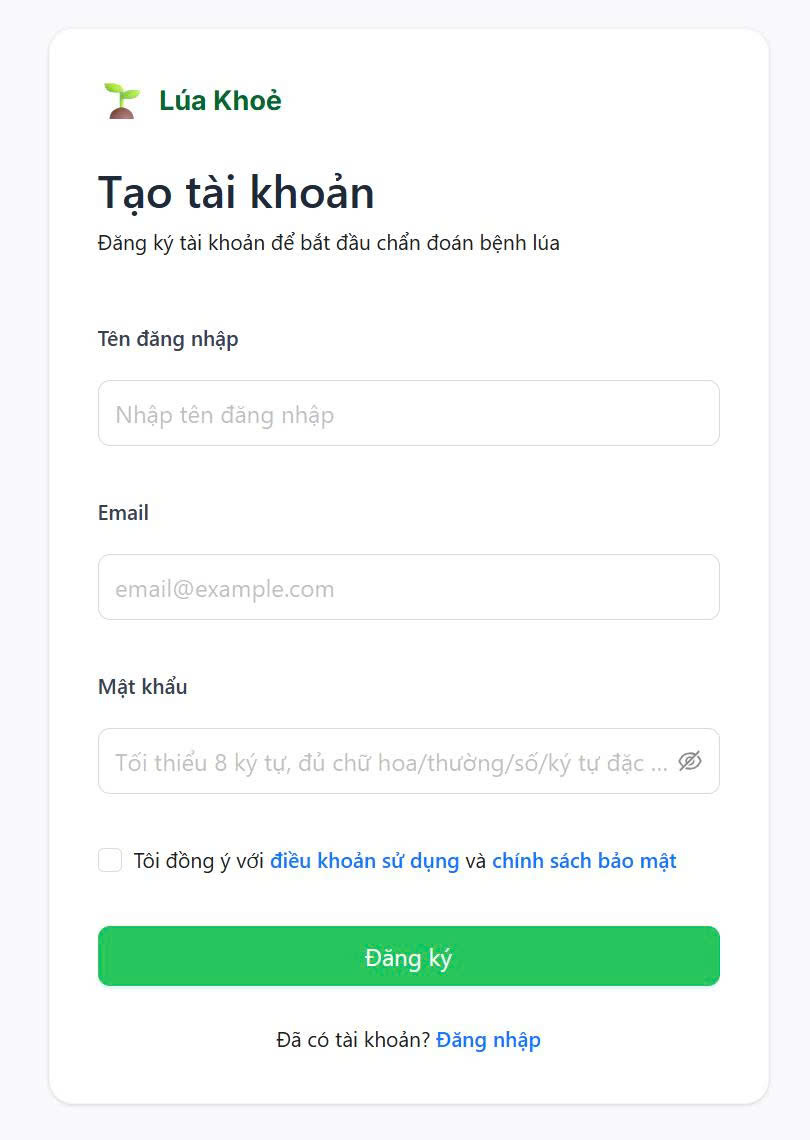
\includegraphics[width=\textwidth,height=0.75\textheight,keepaspectratio]{nd_bm_1.jpg}
    \caption{Giao diện ND\_BM 1: Phiếu đăng ký tài khoản}
    \label{fig:nd-bm-1}
\end{figure}

\vspace{0.3cm}
\noindent\textbf{ND\_BM 1b: ĐĂNG NHẬP HỆ THỐNG}

\begin{figure}[htbp]
    \centering
    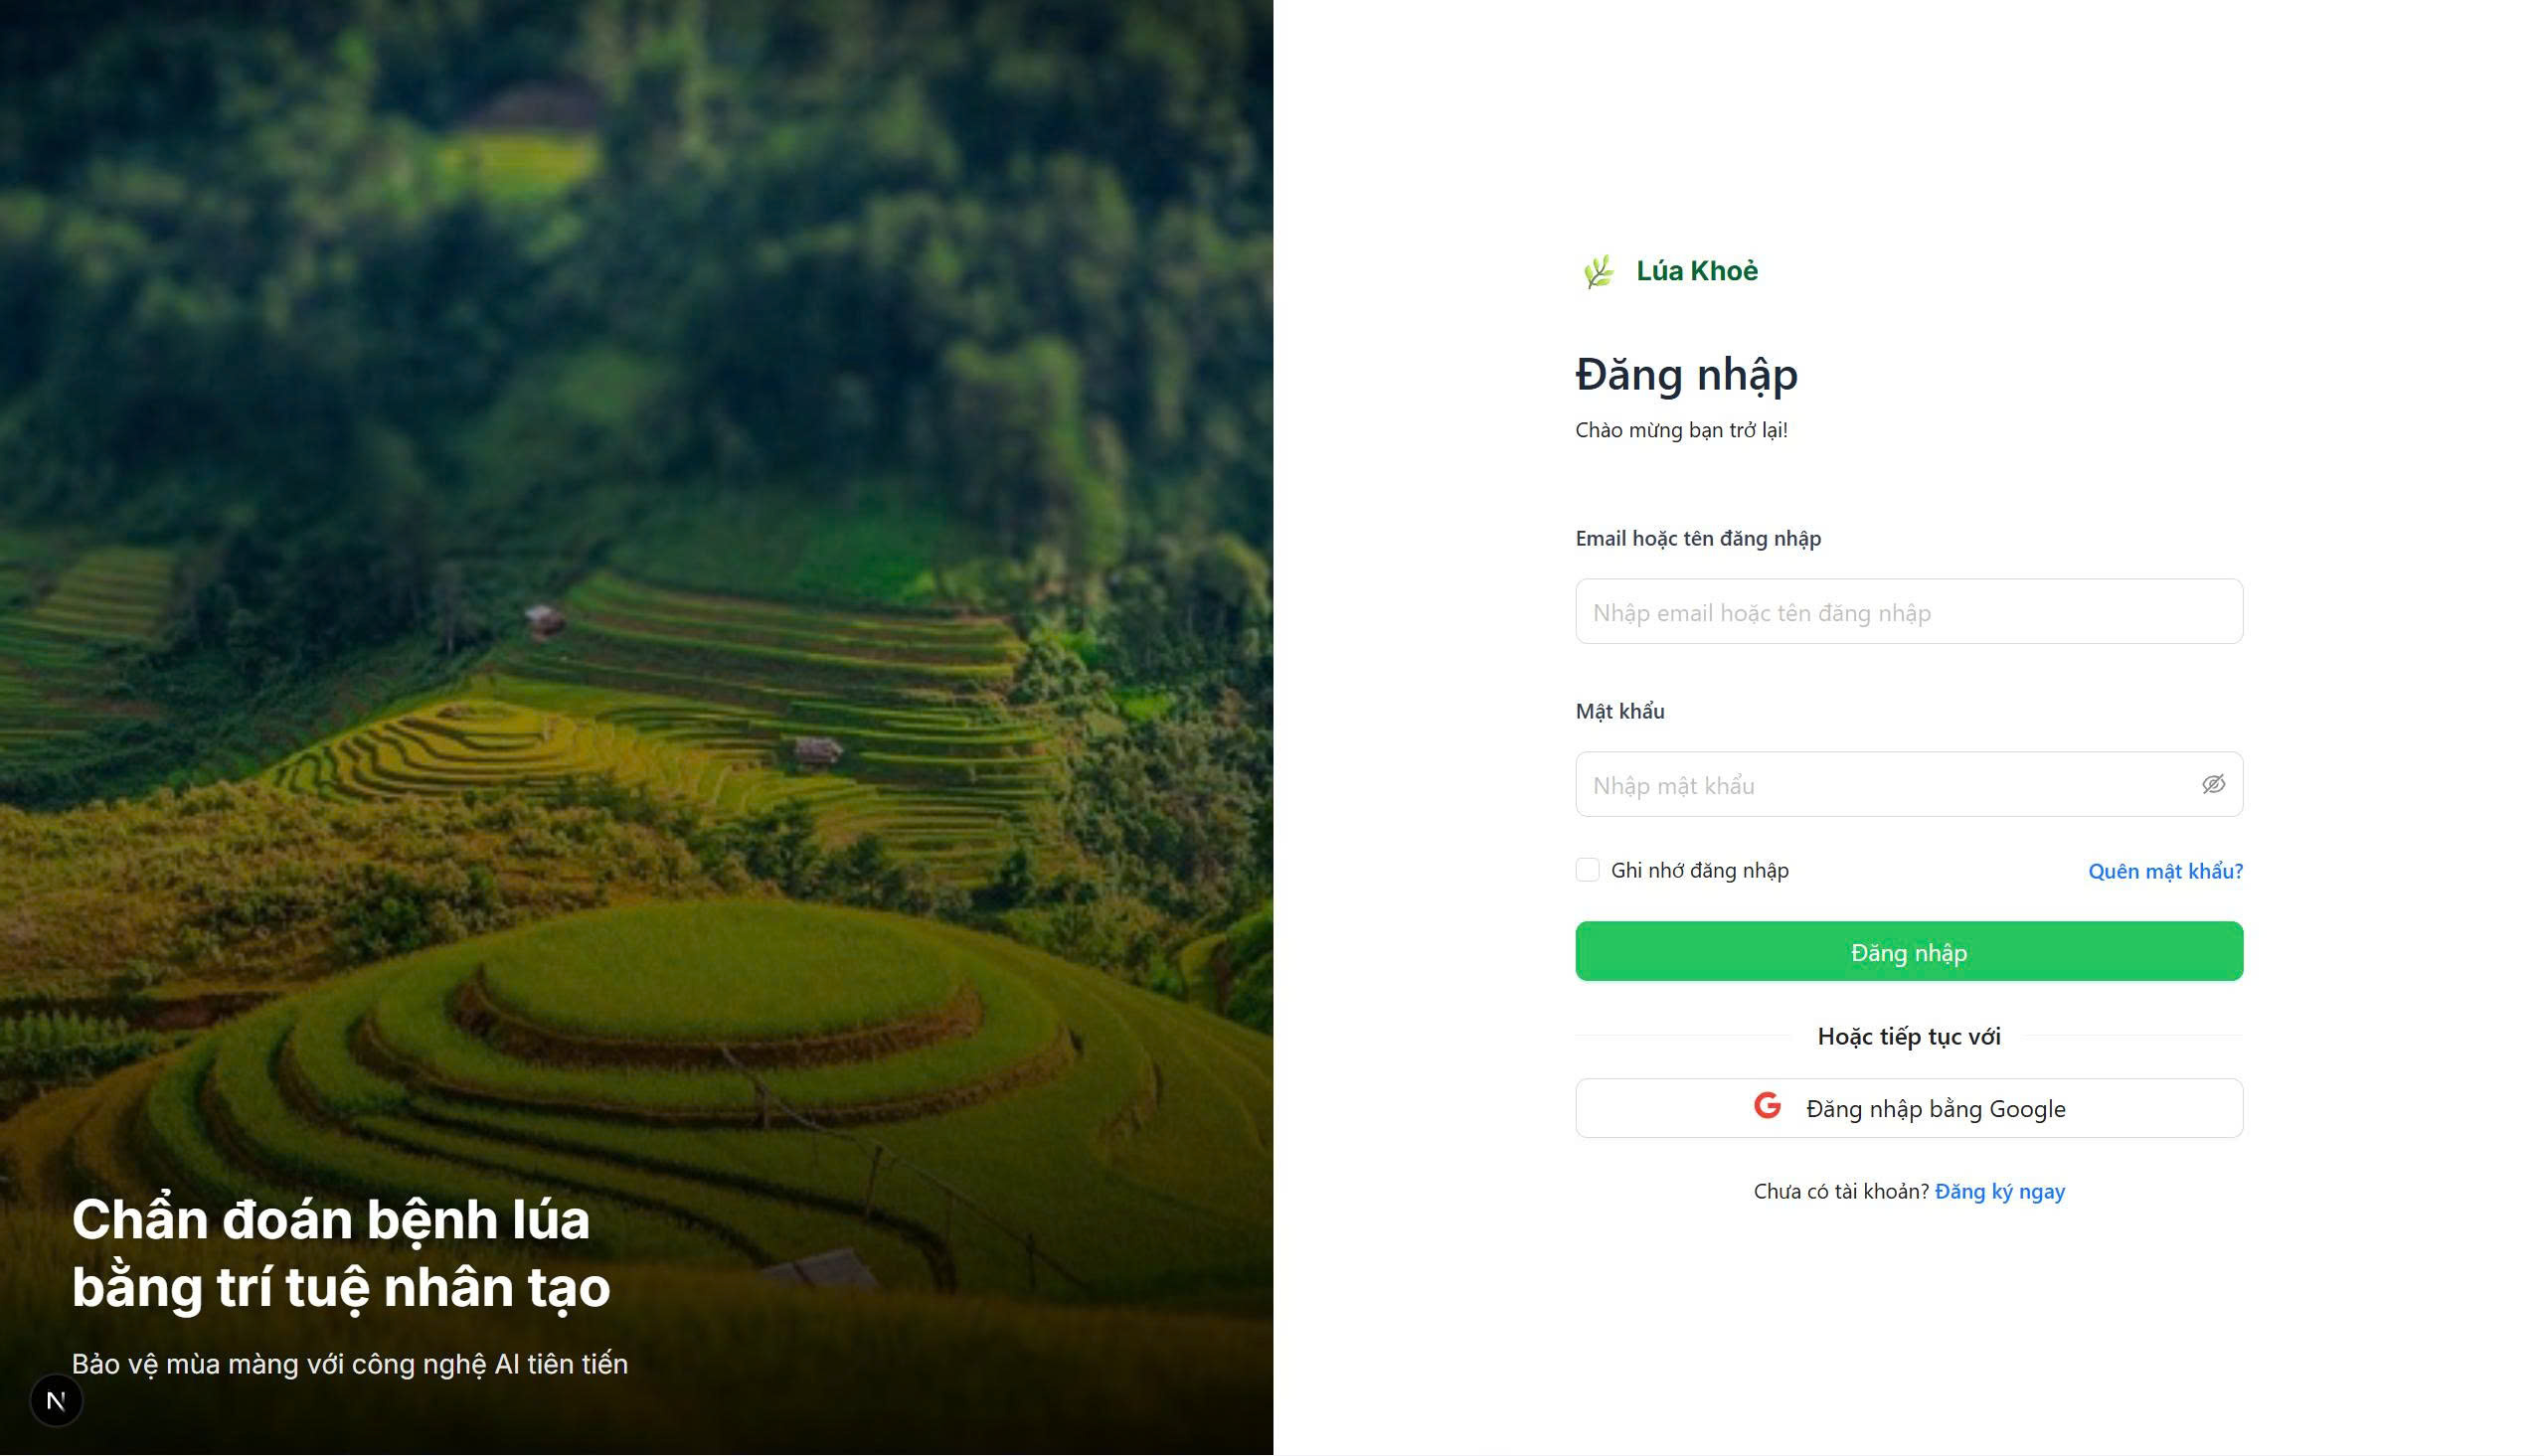
\includegraphics[width=\textwidth,height=0.75\textheight,keepaspectratio]{nd_bm_1b.jpg}
    \caption{Giao diện ND\_BM 1b: Đăng nhập hệ thống}
    \label{fig:nd-bm-1b}
\end{figure}

\vspace{0.3cm}
\noindent\textbf{ND\_BM 1c: ĐỔI MẬT KHẨU}

\begin{figure}[htbp]
    \centering
    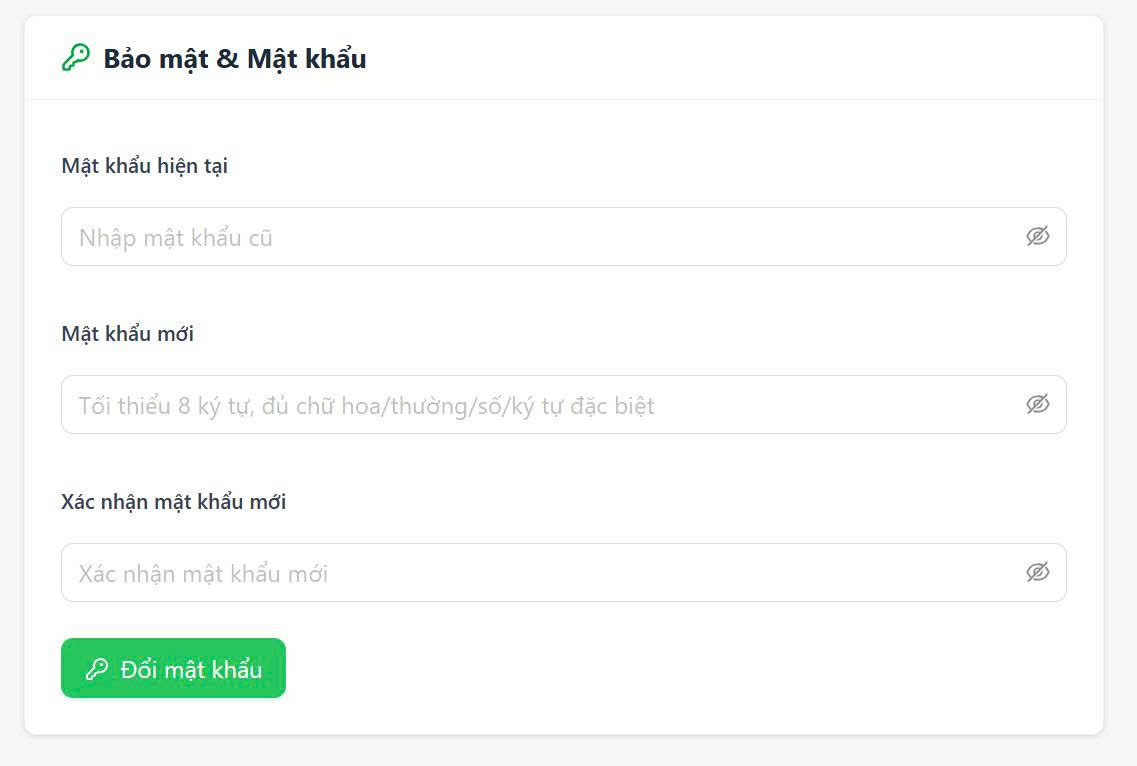
\includegraphics[width=\textwidth,height=0.75\textheight,keepaspectratio]{nd_bm_1c.jpg}
    \caption{Giao diện ND\_BM 1c: Đổi mật khẩu}
    \label{fig:nd-bm-1c}
\end{figure}

\vspace{0.3cm}
\noindent\textbf{ND\_BM 2: PHIẾU CHỈNH SỬA THÔNG TIN CÁ NHÂN}

\begin{figure}[htbp]
    \centering
    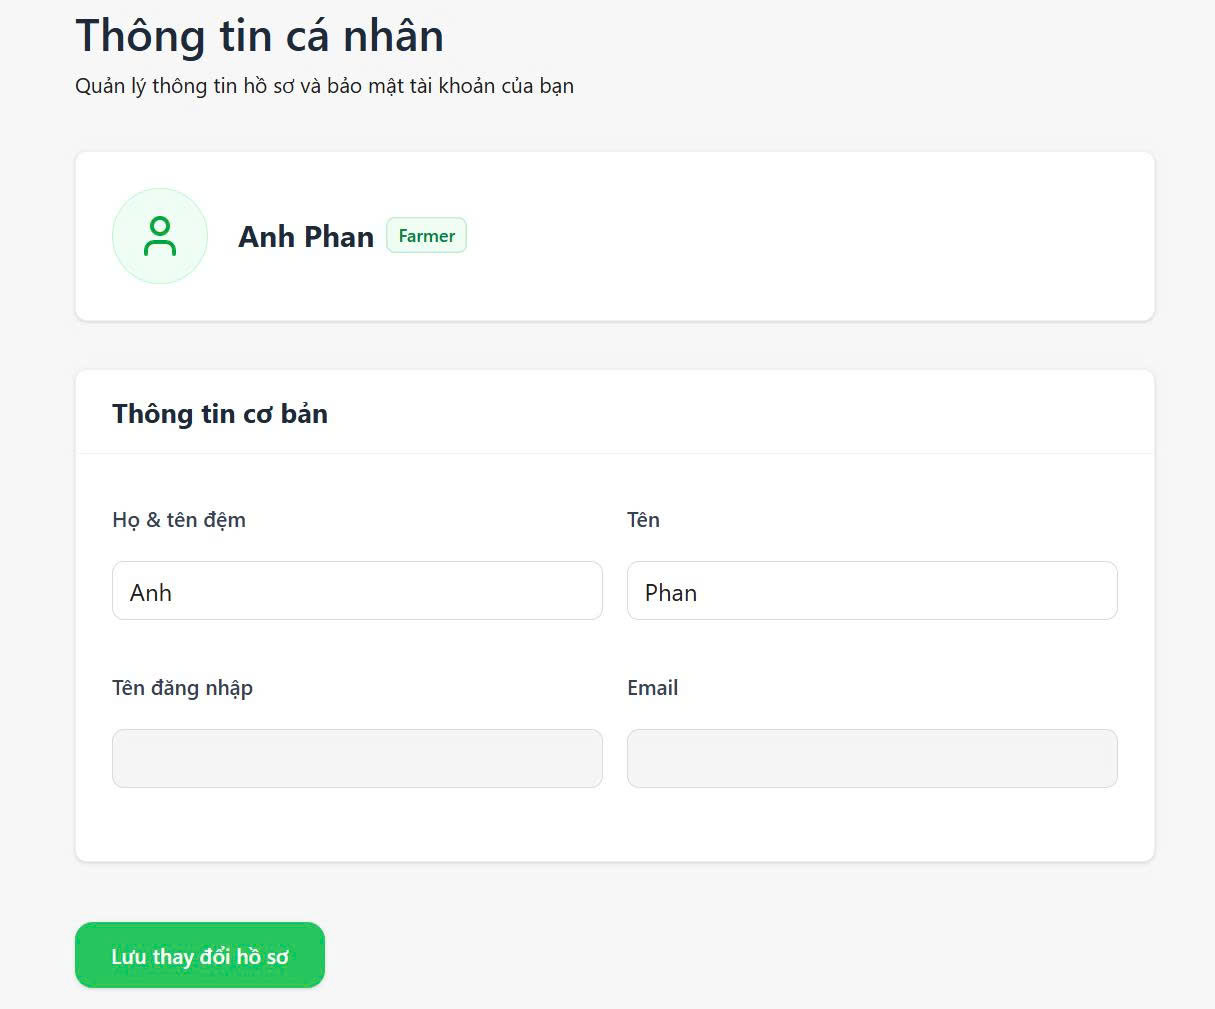
\includegraphics[width=\textwidth,height=0.75\textheight,keepaspectratio]{nd_bm_2.jpg}
    \caption{Giao diện ND\_BM 2: Phiếu chỉnh sửa thông tin cá nhân}
    \label{fig:nd-bm-2}
\end{figure}

\vspace{0.3cm}
\noindent\textbf{ND\_BM 3: PHIẾU GỬI ẢNH CHẨN ĐOÁN}

\begin{figure}[htbp]
    \centering
    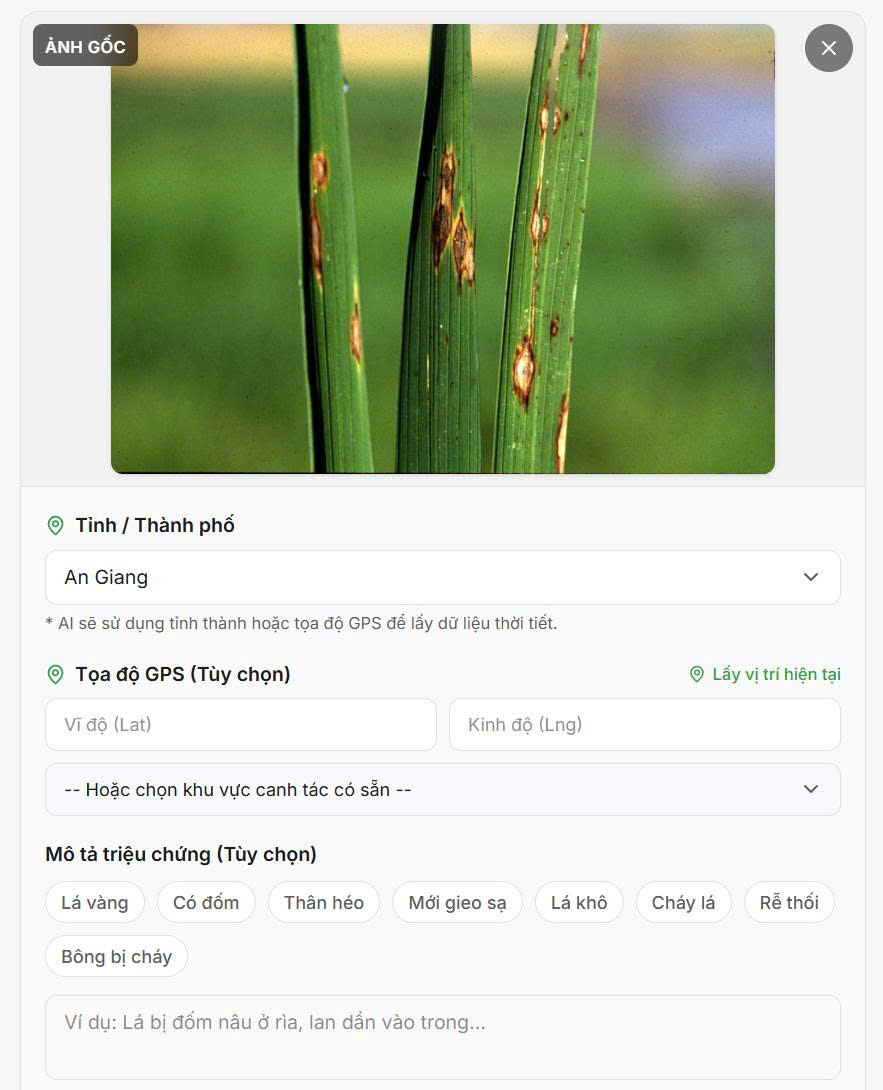
\includegraphics[width=\textwidth,height=0.75\textheight,keepaspectratio]{nd_bm_3.jpg}
    \caption{Giao diện ND\_BM 3: Phiếu gửi ảnh chẩn đoán}
    \label{fig:nd-bm-3}
\end{figure}

\vspace{0.2cm}
\noindent\textbf{ND\_BM 3b: PHIẾU NHẬP THÔNG SỐ MÔI TRƯỜNG} \textit{(tùy chọn)}

\begin{figure}[htbp]
    \centering
    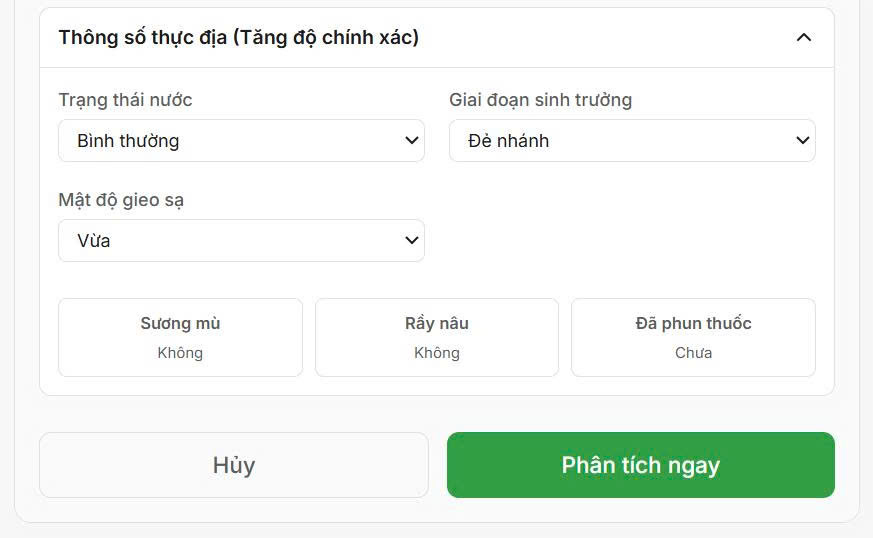
\includegraphics[width=\textwidth,height=0.75\textheight,keepaspectratio]{nd_bm_3b.jpg}
    \caption{Giao diện ND\_BM 3b: Phiếu nhập thông số môi trường (tùy chọn)}
    \label{fig:nd-bm-3b}
\end{figure}

\vspace{0.3cm}
\noindent\textbf{ND\_BM 4: PHIẾU PHẢN HỒI KẾT QUẢ CHẨN ĐOÁN}

\begin{figure}[htbp]
    \centering
    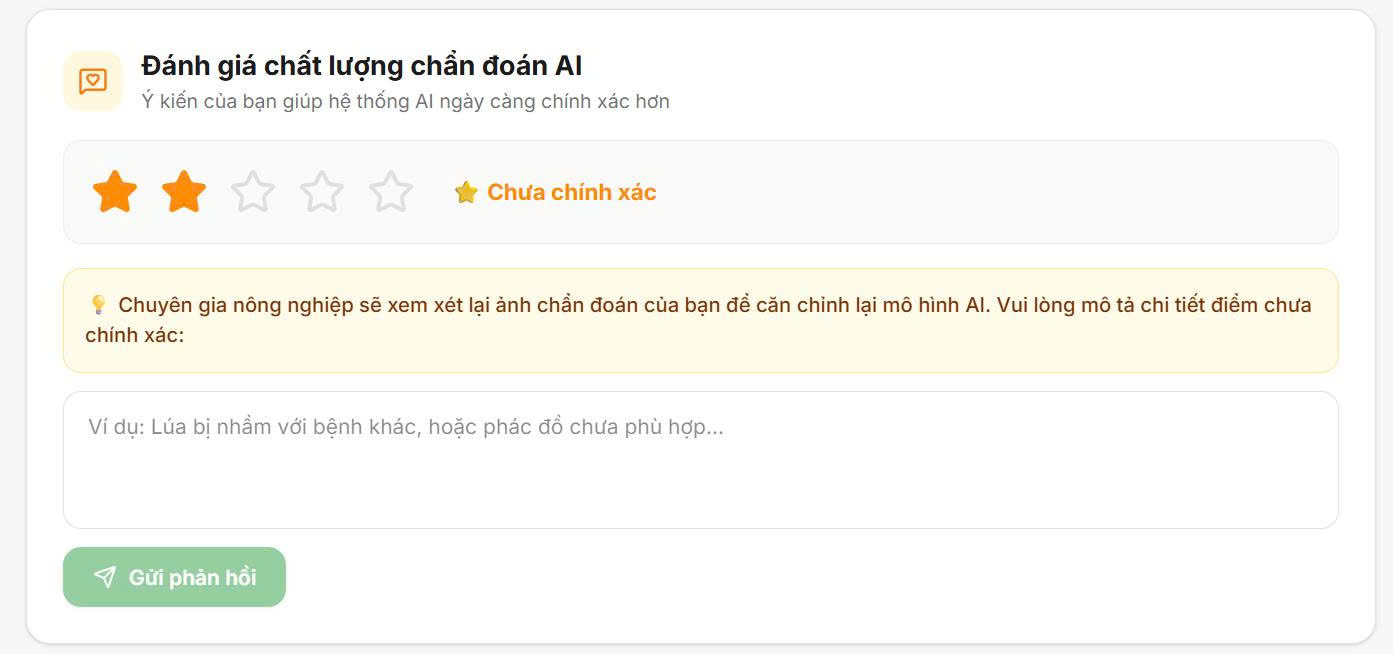
\includegraphics[width=\textwidth,height=0.75\textheight,keepaspectratio]{nd_bm_4.jpg}
    \caption{Giao diện ND\_BM 4: Phiếu phản hồi kết quả chẩn đoán}
    \label{fig:nd-bm-4}
\end{figure}

% ============================================================
% NGƯỜI DÙNG: QUẢN TRỊ VIÊN
% ============================================================
\section{Người dùng --- Quản trị viên (Mã số: AD)}

\textbf{Định nghĩa:} Người sử dụng hệ thống với mục đích quản lý danh mục bệnh lúa, kho tri thức dinh dưỡng, tài khoản người dùng và theo dõi hiệu suất mô hình AI.

\vspace{0.3cm}
\textbf{1. Bảng yêu cầu chức năng nghiệp vụ}

\begin{longtable}{|
        c|
        >{\raggedright\arraybackslash}p{3.2cm}|
        >{\raggedright\arraybackslash}p{2.2cm}|
        >{\raggedright\arraybackslash}p{2.4cm}|
        >{\raggedright\arraybackslash}p{2.6cm}|
        >{\raggedright\arraybackslash}p{2.6cm}|}
    \hline
    \rowcolor{headerblue}
    \textbf{STT} & \textbf{Công việc}          & \textbf{Loại công việc} & \textbf{Quy định/CT liên quan} & \textbf{Biểu mẫu liên quan} & \textbf{Ghi chú} \\
    \hline
    \endhead
    \multicolumn{6}{|l|}{\cellcolor{notegreen}\textbf{I. Tài khoản quản trị}}                                                                              \\
    \hline
    1            & Đăng nhập hệ thống quản trị & Tra cứu                 & QĐ-AD-01                       &                             &                  \\
    \hline
    2            & Đổi mật khẩu quản trị       & Lưu trữ                 & QĐ-AD-01                       &                             &                  \\
    \hline
    \multicolumn{6}{|l|}{\cellcolor{notegreen}\textbf{II. Quản lý bệnh lúa}}                                                                               \\
    \hline
    3            & Quản lý bệnh lúa            & Lưu trữ                 & QĐ-AD-02                       & AD\_BM 1                    &                  \\
    \hline
    \multicolumn{6}{|l|}{\cellcolor{notegreen}\textbf{III. Quản lý tri thức dinh dưỡng}}                                                                   \\
    \hline
    4            & Quản lý tri thức dinh dưỡng & Lưu trữ                 & QĐ-AD-03                       & AD\_BM 2                    &                  \\
    \hline
    \multicolumn{6}{|l|}{\cellcolor{notegreen}\textbf{IV. Quản lý người dùng}}                                                                             \\
    \hline
    5            & Xem danh sách người dùng    & Tra cứu                 & QĐ-AD-04                       &                             &                  \\
    \hline
    6            & Khóa / Mở khóa tài khoản    & Lưu trữ                 & QĐ-AD-04                       &                             &                  \\
    \hline
    \multicolumn{6}{|l|}{\cellcolor{notegreen}\textbf{V. Quản lý phản hồi}}                                                                                \\
    \hline
    7            & Xem danh sách phản hồi      & Tra cứu                 & QĐ-AD-05                       &                             &                  \\
    \hline
    8            & Xử lý phản hồi              & Lưu trữ                 & QĐ-AD-05                       & AD\_BM 3                    &                  \\
    \hline
    \multicolumn{6}{|l|}{\cellcolor{notegreen}\textbf{VI. Hệ thống}}                                                                                       \\
    \hline
    9            & Cập nhật mô hình AI         & Lưu trữ                 & QĐ-AD-06                       &                             &                  \\
    \hline
    10           & Xem thống kê \& báo cáo     & Tra cứu, Kết xuất       & QĐ-AD-06                       & AD\_BM 4                    &                  \\
    \hline
\end{longtable}

% ============================================================
\vspace{0.3cm}
\textbf{2. Bảng Quy định / Công thức liên quan --- Quản trị viên}

\begin{longtable}{|
        c|
        >{\raggedright\arraybackslash}p{1.8cm}|
        >{\raggedright\arraybackslash}p{3.4cm}|
        >{\raggedright\arraybackslash}p{6.4cm}|
        >{\raggedright\arraybackslash}p{1.4cm}|}
    \hline
    \rowcolor{headerblue}
    \textbf{STT} & \textbf{Mã số} & \textbf{Tên Quy định}                & \textbf{Mô tả chi tiết}                                                                                                & \textbf{Ghi chú} \\
    \hline
    \endhead
    1            & QĐ-AD-01       & Quy định Tài khoản quản trị          & Bao gồm quy trình đăng nhập (kiểm tra cặp tên đăng nhập + mật khẩu, khóa sau 5 lần sai trong 30 phút) và đổi mật khẩu. &                  \\
    \hline
    2            & QĐ-AD-02       & Quy định Quản lý bệnh lúa            & Bao gồm quy trình thêm, sửa, ẩn/xóa bệnh lúa. Tên bệnh duy nhất, xóa vĩnh viễn chỉ khi chưa có lịch sử.                &                  \\
    \hline
    3            & QĐ-AD-03       & Quy định Quản lý tri thức dinh dưỡng & Bao gồm quy trình thêm, sửa, xóa thông tin dinh dưỡng. Mỗi bản ghi phải gắn với một loại bệnh cụ thể.                  &                  \\
    \hline
    4            & QĐ-AD-04       & Quy định Quản lý người dùng          & Bao gồm quy trình xem danh sách người dùng và khóa/mở khóa tài khoản. Admin không được chỉnh sửa thông tin người dùng. &                  \\
    \hline
    5            & QĐ-AD-05       & Quy định Xử lý phản hồi              & Bao gồm quy trình xem danh sách phiếu phản hồi, xem xét kết quả và chốt trạng thái xử lý.                              &                  \\
    \hline
    6            & QĐ-AD-06       & Quy định Hệ thống                    & Bao gồm quy trình cập nhật mô hình AI và xem thống kê/báo cáo hiệu suất.                                               &                  \\
    \hline
\end{longtable}

% ============================================================
\vspace{0.3cm}
\textbf{3. Chi tiết từng Quy định --- Quản trị viên}

\vspace{0.3cm}
\noindent\textbf{QĐ-AD-01 --- Quy định Tài khoản quản trị}

\noindent\textit{a) Đăng nhập hệ thống quản trị}

\noindent\textbf{Quy trình đăng nhập:}
\begin{enumerate}
    \item Quản trị viên nhập 2 thông tin: tên đăng nhập và mật khẩu.
    \item Hệ thống kiểm tra mật khẩu có đúng với tên đăng nhập đã nhập hay không.
    \item Nếu sai, hệ thống thông báo chung ``Tên đăng nhập hoặc mật khẩu không chính xác''. Nhập sai 5 lần liên tiếp thì khóa tài khoản 30 phút.
    \item Nếu đúng, đăng nhập thành công vào trang quản trị.
\end{enumerate}

\noindent\textit{b) Đổi mật khẩu}

\noindent\textbf{Quy trình đổi mật khẩu:}
\begin{enumerate}
    \item Nhập mật khẩu hiện tại để xác thực.
    \item Nhập mật khẩu mới --- phải đáp ứng độ mạnh (tối thiểu 8 ký tự, gồm chữ hoa, chữ số và ký tự đặc biệt) và không được trùng mật khẩu cũ.
    \item Nhập xác nhận mật khẩu mới --- phải gõ chính xác giống bước 2.
\end{enumerate}

\vspace{0.3cm}
\noindent\textbf{QĐ-AD-02 --- Quy định Quản lý bệnh lúa}

\noindent\textbf{Định nghĩa:} Bản ghi bệnh lúa gồm 3 thông tin: tên bệnh (tiếng Việt), tên khoa học và mô tả triệu chứng.

\noindent\textbf{Quy trình quản lý:}
\begin{enumerate}
    \item \textbf{Thêm bệnh:} Nhập đầy đủ 3 thông tin. Tên bệnh và tên khoa học phải là duy nhất trong hệ thống.
    \item \textbf{Sửa bệnh:} Chỉnh sửa thông tin bệnh nhưng không được thay đổi mã định danh hệ thống.
    \item \textbf{Xóa / Ẩn bệnh:} Nếu bệnh chưa có dữ liệu lịch sử chẩn đoán thì xóa vĩnh viễn. Nếu đã có lịch sử thì chỉ được chuyển sang trạng thái ``Ẩn''.
\end{enumerate}

\vspace{0.3cm}
\noindent\textbf{QĐ-AD-03 --- Quy định Quản lý tri thức dinh dưỡng}

\noindent\textbf{Định nghĩa:} Bản ghi dinh dưỡng gồm: bệnh lúa áp dụng (bắt buộc), nội dung tri thức (hoạt chất, hướng dẫn sử dụng).

\noindent\textbf{Quy trình quản lý:}
\begin{enumerate}
    \item \textbf{Thêm:} Chọn bệnh lúa từ danh mục, nhập nội dung tri thức. Mỗi bản ghi phải gắn với một loại bệnh cụ thể.
    \item \textbf{Sửa:} Cập nhật nội dung tri thức. Hệ thống tự động cập nhật dữ liệu tìm kiếm ngữ nghĩa.
    \item \textbf{Xóa:} Xóa bản ghi khỏi kho tri thức. Thay đổi có hiệu lực ngay lập tức.
\end{enumerate}

\vspace{0.3cm}
\noindent\textbf{QĐ-AD-04 --- Quy định Quản lý người dùng}

\noindent\textit{a) Xem danh sách người dùng}

Hệ thống hiển thị danh sách người dùng với thông tin định danh: tên đăng nhập, email, số lượt chẩn đoán, số lượt phản hồi và trạng thái tài khoản.

\noindent\textit{b) Khóa / Mở khóa tài khoản}

\noindent\textbf{Quy trình:}
\begin{enumerate}
    \item Quản trị viên chọn tài khoản cần thay đổi trạng thái.
    \item Chuyển trạng thái giữa ``Hoạt động'' và ``Tạm khóa''.
\end{enumerate}
\noindent\textbf{Ràng buộc:} Quản trị viên không được chỉnh sửa tên đăng nhập, email hoặc bất kỳ thông tin cá nhân nào của người dùng.

\vspace{0.3cm}
\noindent\textbf{QĐ-AD-05 --- Quy định Xử lý phản hồi}

\noindent\textbf{Quy trình xử lý:}
\begin{enumerate}
    \item Xem danh sách phiếu chưa xử lý, ưu tiên phiếu gửi sớm nhất.
    \item Xem xét song song: ảnh gốc, kết quả AI và kết quả nông dân báo cáo.
    \item Nhập lời nhắn phản hồi gửi lại cho nông dân.
    \item Chốt trạng thái xử lý: ``Chấp nhận'' (AI sai) hoặc ``Từ chối'' (AI đúng).
\end{enumerate}
\noindent\textbf{Ràng buộc:} Nếu chọn ``Chấp nhận'', hệ thống tự động lưu ảnh vào tập dữ liệu để nâng cấp mô hình AI sau này.

\vspace{0.3cm}
\noindent\textbf{QĐ-AD-06 --- Quy định Hệ thống}

\noindent\textit{a) Cập nhật mô hình AI}

\noindent\textbf{Quy trình cập nhật:}
\begin{enumerate}
    \item Tải lên file mô hình AI mới kèm tên phiên bản và ghi chú thay đổi.
    \item Hệ thống lưu file mô hình ở trạng thái chưa kích hoạt.
    \item Quản trị viên dùng công tắc ``Kích hoạt'' để áp dụng mô hình mới cho toàn hệ thống. Mô hình cũ tự động tắt.
\end{enumerate}

\noindent\textit{b) Thống kê \& Báo cáo}

Hệ thống hiển thị 2 loại báo cáo:
\begin{itemize}
    \item \textbf{Bản đồ dịch bệnh:} bản đồ nhiệt tình hình dịch bệnh theo tọa độ GPS của các ca chẩn đoán.
    \item \textbf{Hiệu suất AI:} thống kê tỷ lệ chẩn đoán đúng/sai theo từng loại bệnh dựa trên kết quả xử lý phản hồi.
\end{itemize}

% ============================================================
\vspace{0.3cm}
\textbf{4. Các Biểu mẫu --- Quản trị viên}

\vspace{0.3cm}
\noindent\textbf{AD\_BM 1: PHIẾU QUẢN LÝ BỆNH LÚA}

\begin{figure}[H]
    \centering
    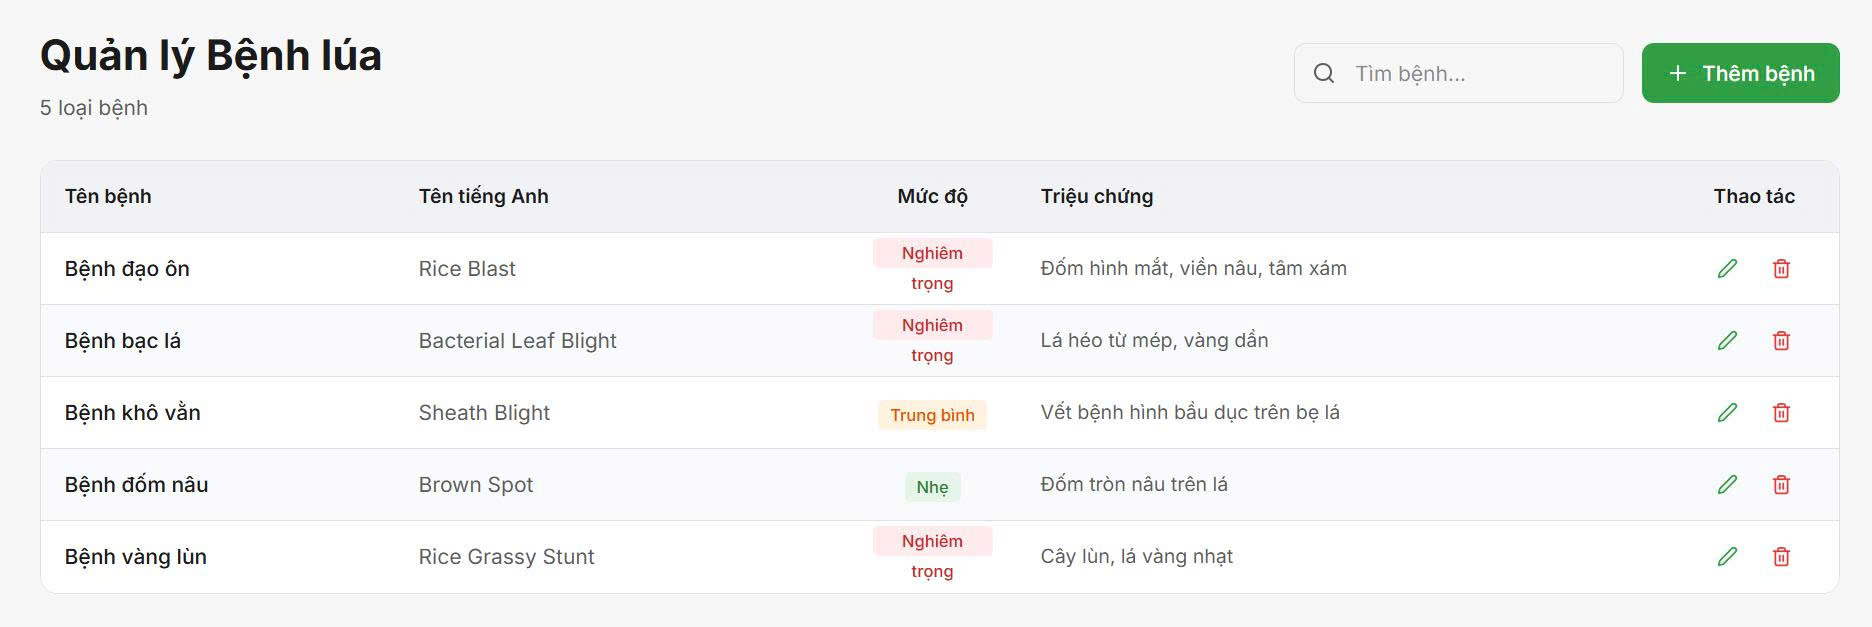
\includegraphics[width=\textwidth,height=0.75\textheight,keepaspectratio]{ad_bm_1.jpg}
    \caption{Giao diện AD\_BM 1: Phiếu quản lý bệnh lúa}
    \label{fig:ad-bm-1}
\end{figure}

\vspace{0.3cm}
\noindent\textbf{AD\_BM 2: PHIẾU QUẢN LÝ TRI THỨC DINH DƯỠNG}

\begin{figure}[H]
    \centering
    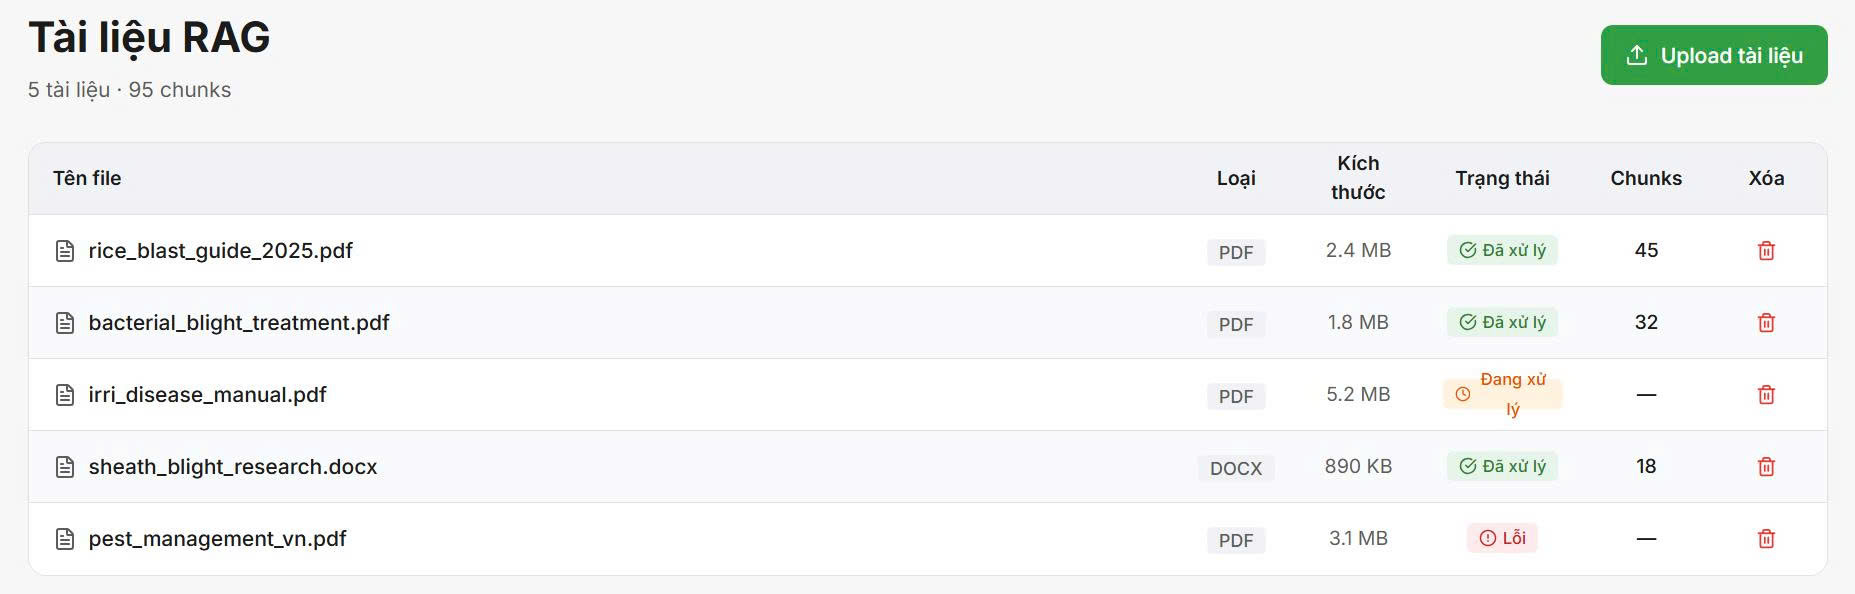
\includegraphics[width=\textwidth,height=0.75\textheight,keepaspectratio]{ad_bm_2.jpg}
    \caption{Giao diện AD\_BM 2: Phiếu quản lý tri thức dinh dưỡng}
    \label{fig:ad-bm-2}
\end{figure}

\vspace{0.3cm}
\noindent\textbf{AD\_BM 3: PHIẾU XỬ LÝ PHẢN HỒI}

\begin{figure}[H]
    \centering
    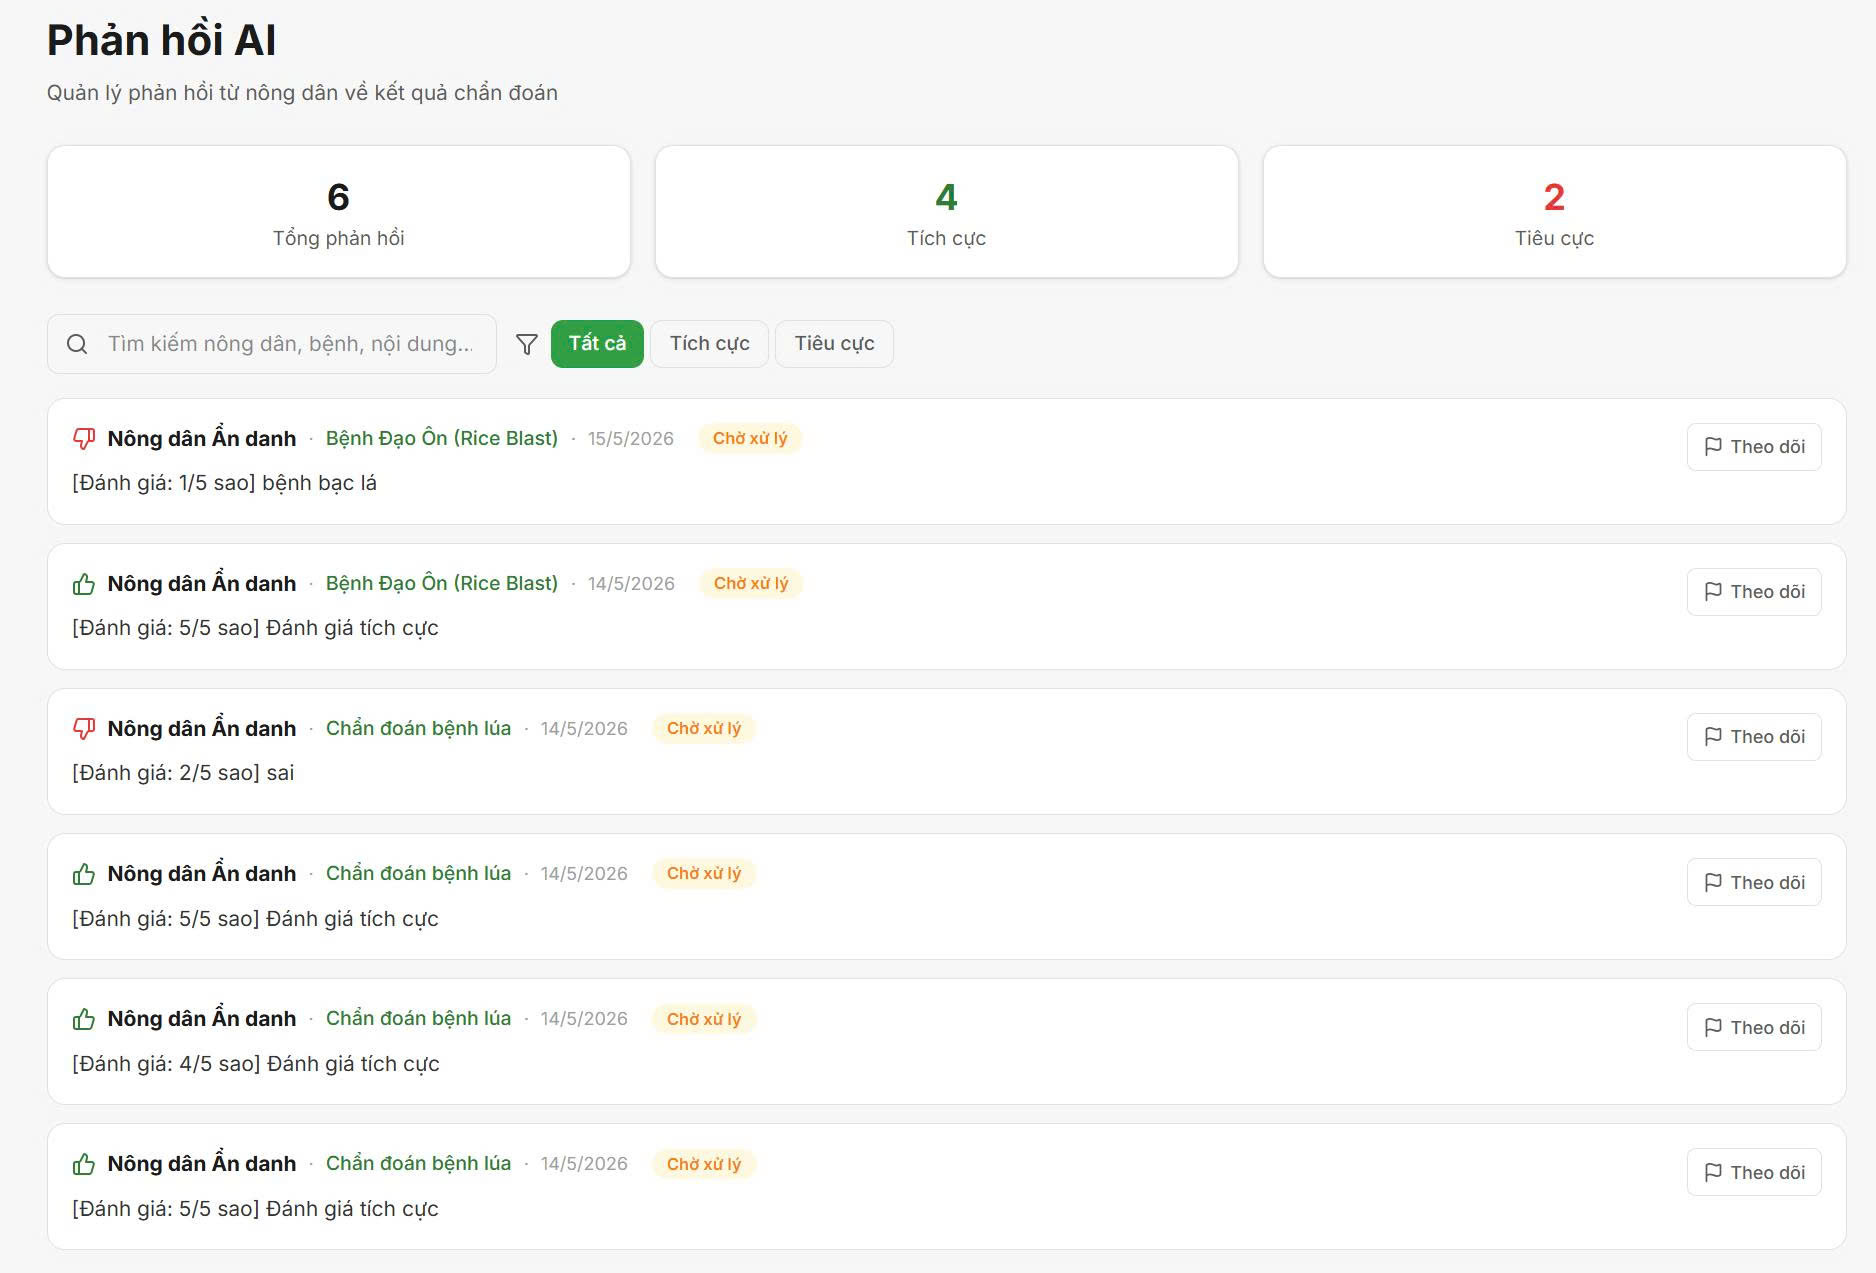
\includegraphics[width=\textwidth,height=0.75\textheight,keepaspectratio]{ad_bm_3.jpg}
    \caption{Giao diện AD\_BM 3: Phiếu xử lý phản hồi}
    \label{fig:ad-bm-3}
\end{figure}

\vspace{0.3cm}
\noindent\textbf{AD\_BM 4: BÁO CÁO HIỆU SUẤT AI}

\begin{figure}[H]
    \centering
    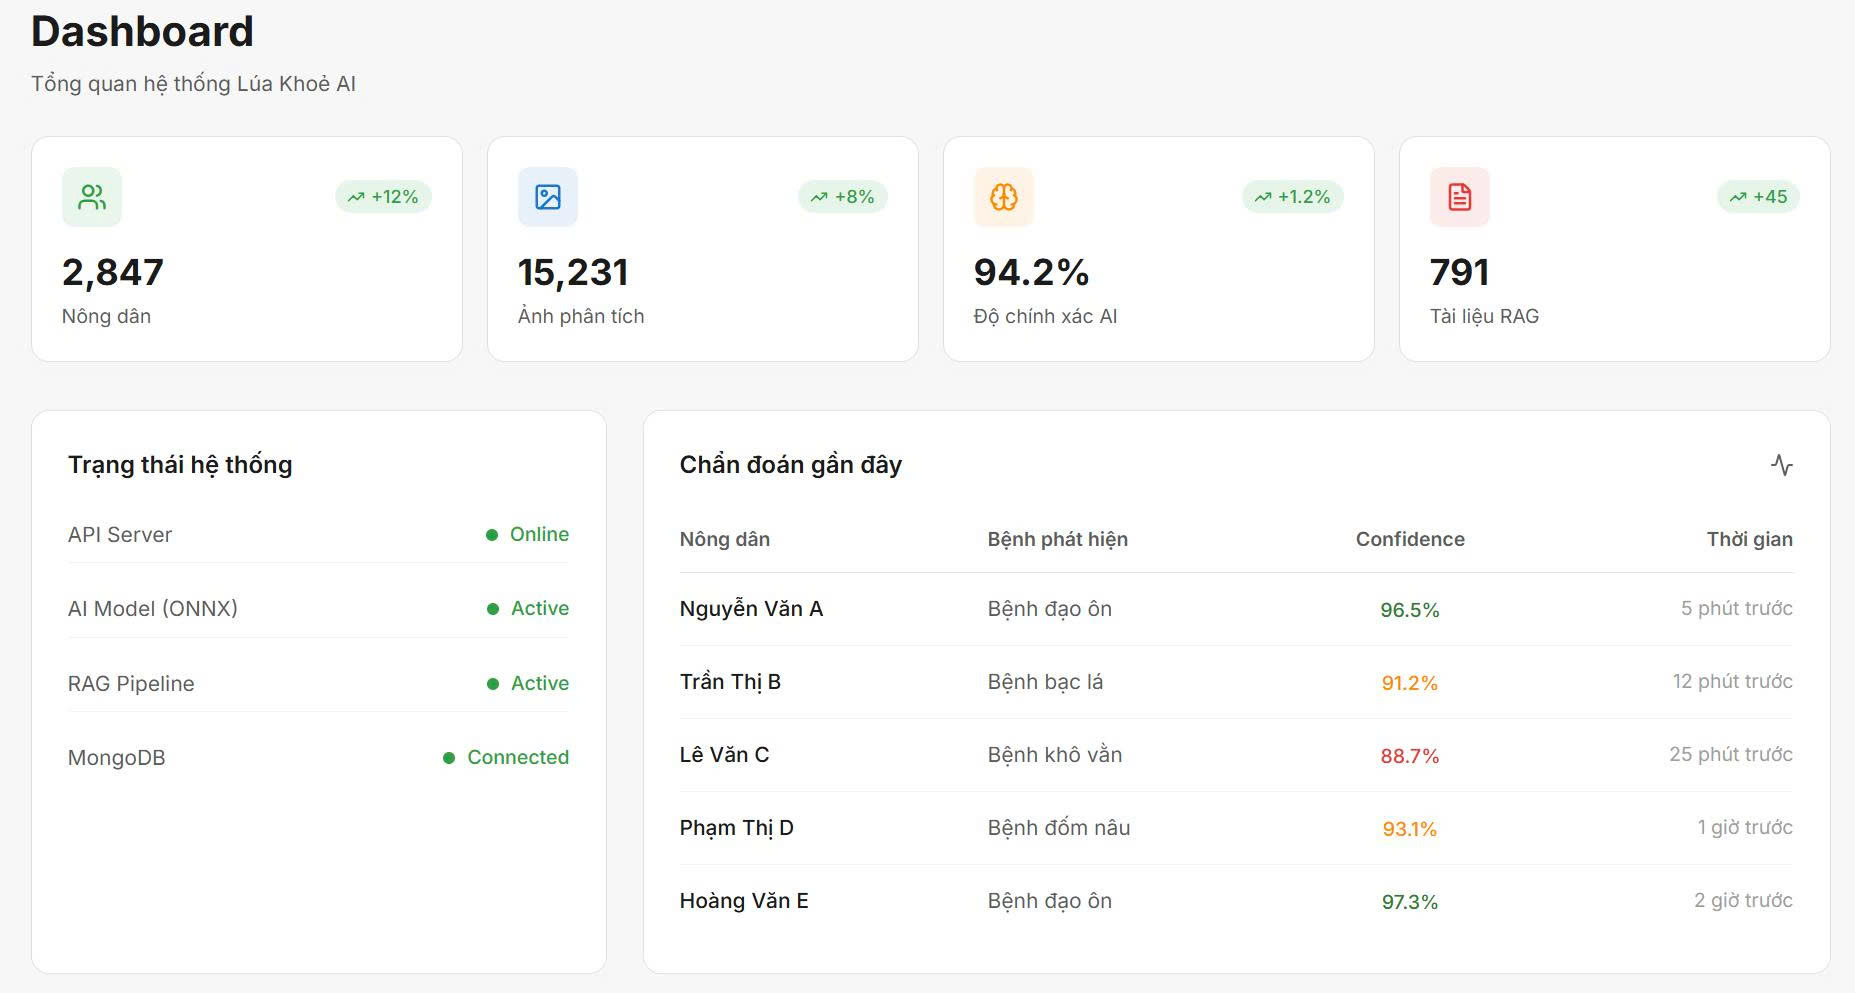
\includegraphics[width=\textwidth,height=0.75\textheight,keepaspectratio]{ad_bm_4.jpg}
    \caption{Giao diện AD\_BM 4: Báo cáo hiệu suất AI}
    \label{fig:ad-bm-4}
\end{figure}

\hrulefill

% ============================================================
\subsubsection{Xác định yêu cầu chức năng hệ thống và yêu cầu chất lượng}

\textbf{Bảng yêu cầu chức năng hệ thống:}
\begin{longtable}{|c|l|p{9.5cm}|l|}
    \hline
    \rowcolor{headerblue}
    \textbf{STT} & \textbf{Nội dung}  & \textbf{Mô tả chi tiết}                                                                            & \textbf{Ghi chú} \\
    \hline
    \endhead
    1            & Tích hợp thời tiết & Truy xuất dữ liệu thời tiết dựa trên tọa độ thực tế của nông dân để cung cấp bối cảnh môi trường.  &                  \\
    \hline
    2            & Quản lý tri thức   & Hệ thống đồng bộ các hướng dẫn dinh dưỡng để AI có thể tư vấn linh hoạt.                           &                  \\
    \hline
    3            & Bảo mật dữ liệu    & Mật khẩu được bảo mật an toàn. Toàn bộ ảnh và dữ liệu thực tế được lưu trữ phục vụ tái huấn luyện. &                  \\
    \hline
    4            & Gửi mã xác thực    & Tự động gửi mã xác thực qua email cho các luồng xác minh tài khoản.                                &                  \\
    \hline
\end{longtable}

\textbf{Bảng yêu cầu về chất lượng hệ thống:}
\begin{longtable}{|c|l|l|p{6.5cm}|l|}
    \hline
    \rowcolor{headerblue}
    \textbf{STT} & \textbf{Nội dung} & \textbf{Tiêu chuẩn} & \textbf{Mô tả chi tiết}                                                    & \textbf{Ghi chú} \\
    \hline
    \endhead
    1            & Cập nhật mô hình  & Tiến hóa            & Có thể thay thế mô hình nhận diện mới mà không làm gián đoạn người dùng.   &                  \\
    \hline
    2            & Tính tiện dụng    & Tiện dụng           & Giao diện tối ưu cho thiết bị di động, thông báo rõ ràng bằng tiếng Việt.  &                  \\
    \hline
    3            & Tốc độ xử lý      & Hiệu quả            & Phản hồi kết quả chẩn đoán trong vòng 5--7 giây.                           &                  \\
    \hline
    4            & Độ tương thích    & Tương thích         & Hoạt động ổn định trên các trình duyệt phổ biến của điện thoại thông minh. &                  \\
    \hline
    5            & Tính kịp thời     & Hiệu quả            & Mã xác thực gửi đến người dùng trong vòng 30 giây.                         &                  \\
    \hline
\end{longtable}

\hrulefill

% ============================================================
\section{Biểu đồ Use Case}

\subsection{Danh sách các tác nhân}

\begin{longtable}{|c|l|p{3.5cm}|p{7.5cm}|}
    \caption{Danh sách các tác nhân trong hệ thống} \\
    \hline
    \rowcolor{headerblue}
    \textbf{STT} & \textbf{Tên tác nhân} & \textbf{Loại tác nhân} & \textbf{Mô tả tóm tắt} \\
    \hline
    \endhead
    1            & Nông dân              & Tác nhân chính (người dùng) & Người sử dụng ứng dụng để chẩn đoán bệnh lúa và nhận gợi ý dinh dưỡng. \\
    \hline
    2            & Quản trị viên         & Tác nhân chính (người dùng) & Người vận hành hệ thống, quản lý dữ liệu và mô hình AI. \\
    \hline
    3            & Weather API           & Tác nhân ngoại vi (hệ thống) & Dịch vụ bên thứ ba cung cấp dữ liệu thời tiết theo tọa độ GPS. \\
    \hline
    4            & Email Service         & Tác nhân ngoại vi (hệ thống) & Dịch vụ gửi email tự động (OTP, xác thực tài khoản). \\
    \hline
\end{longtable}

\subsection{Mô tả chi tiết từng tác nhân}

\textbf{Tác nhân 1 --- Nông dân (ND):} \\
Nông dân là người dùng cuối của hệ thống, sử dụng ứng dụng trên thiết bị di động. Nông dân không cần kiến thức kỹ thuật; giao diện được tối ưu cho người dùng phổ thông. Nông dân tương tác với hệ thống qua các chức năng: đăng ký/đăng nhập, gửi ảnh lúa để chẩn đoán, xem kết quả và gợi ý dinh dưỡng, tra cứu lịch sử chẩn đoán, và gửi phản hồi nếu kết quả chưa chính xác.

\vspace{0.3cm}
\textbf{Tác nhân 2 --- Quản trị viên (AD):} \\
Quản trị viên là người vận hành và duy trì hệ thống, có tài khoản được cấp sẵn (không tự đăng ký). Quản trị viên có toàn quyền trên dữ liệu hệ thống: quản lý danh mục bệnh lúa, kho tri thức dinh dưỡng, tài khoản người dùng, xử lý phản hồi từ nông dân và cập nhật mô hình AI. Quản trị viên không thể chỉnh sửa thông tin cá nhân của người dùng.

\vspace{0.3cm}
\textbf{Tác nhân 3 --- Weather API (Hệ thống thời tiết):} \\
Là dịch vụ thời tiết bên thứ ba (ví dụ: OpenWeatherMap). Hệ thống tự động gọi API này khi nông dân gửi ảnh chẩn đoán, sử dụng tọa độ GPS lưu trong hồ sơ (hoặc vị trí bổ sung nếu có) để lấy dữ liệu nhiệt độ, độ ẩm phục vụ chẩn đoán. Đây là tác nhân bị động --- chỉ phản hồi khi được hệ thống gọi, không chủ động khởi tạo tương tác.

\vspace{0.3cm}
\textbf{Tác nhân 4 --- Email Service (Dịch vụ email):} \\
Là dịch vụ gửi email tự động bên thứ ba (ví dụ: SendGrid, AWS SES). Hệ thống gọi dịch vụ này trong 3 luồng: gửi mã OTP xác thực khi đăng ký, gửi liên kết/mã khi khôi phục mật khẩu. Tương tự Weather API, đây là tác nhân bị động, chỉ thực thi khi được hệ thống yêu cầu.

\hrulefill

\subsection{Biểu đồ Use Case tổng quát}

% Chèn ảnh Use Case tổng quát (xuất từ Mermaid/draw.io)
\begin{figure}[htbp]
    \centering
    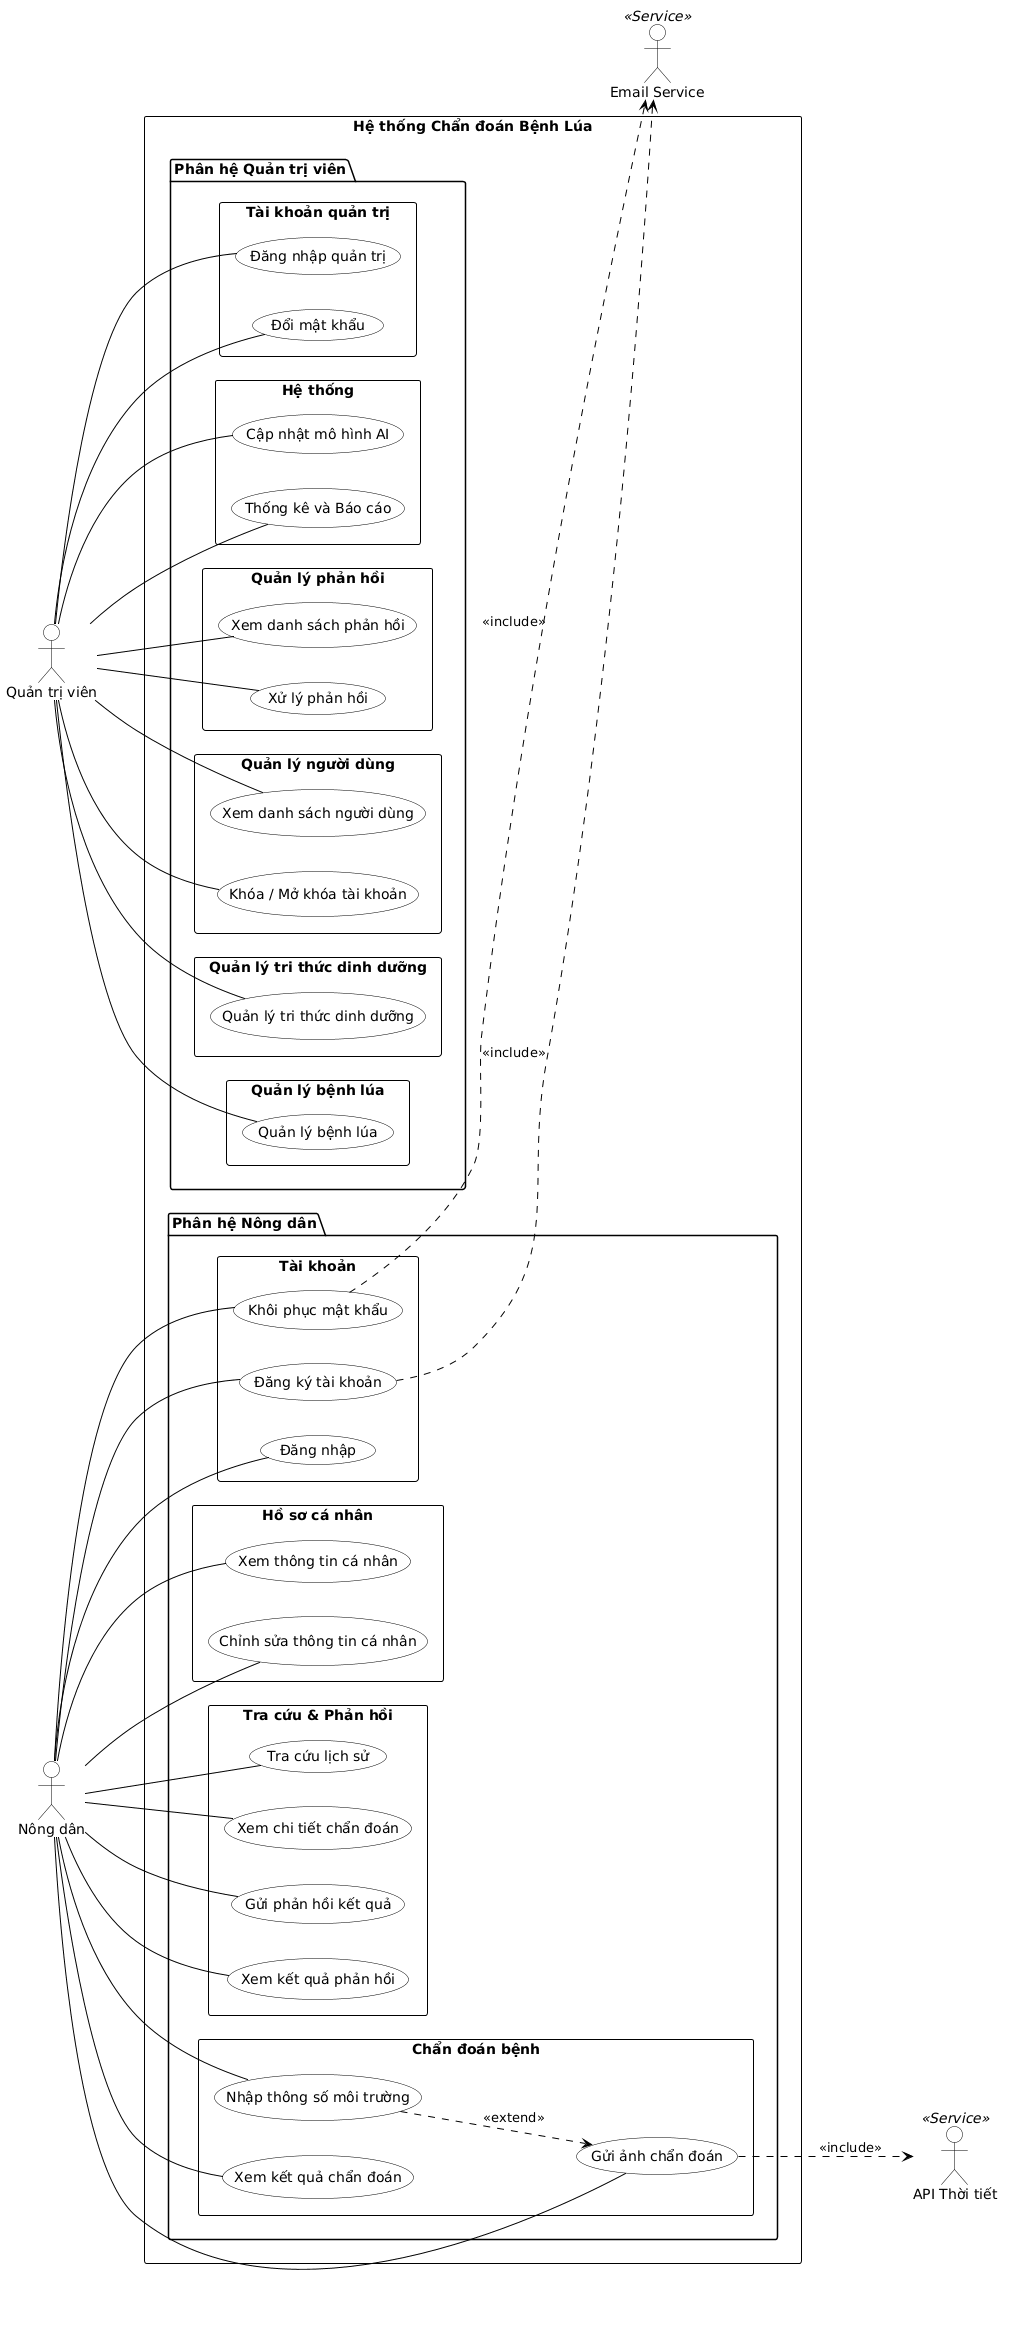
\includegraphics[width=\textwidth,height=0.85\textheight,keepaspectratio]{usecase-tong-quat.png}
    \caption{Biểu đồ Use Case tổng quát của hệ thống}
    \label{fig:usecase-tong-quat}
\end{figure}

\subsection{Bảng ký hiệu UML}

\begin{longtable}{|l|p{11cm}|}
    \hline
    \rowcolor{headerblue}
    \textbf{Ký hiệu}                       & \textbf{Ý nghĩa}                            \\
    \hline
    Hình người (stick figure)              & Actor --- tác nhân tương tác với hệ thống   \\
    \hline
    Hình elip                              & Use Case --- chức năng hệ thống             \\
    \hline
    Hình chữ nhật bao quanh                & System Boundary --- ranh giới hệ thống      \\
    \hline
    Đường liền                             & Association --- actor sử dụng use case      \\
    \hline
    Mũi tên đứt nét + \texttt{<<include>>} & Use case bắt buộc gọi đến use case khác     \\
    \hline
    Mũi tên đứt nét + \texttt{<<extend>>}  & Use case mở rộng (tùy chọn, không bắt buộc) \\
    \hline
\end{longtable}

\subsection{Các biểu đồ Use Case phân rã}

% --- Phân rã Nông dân (ND) ---
\subsubsection{Các Use Case của Nông dân (ND)}

\begin{figure}[htbp]
    \centering
    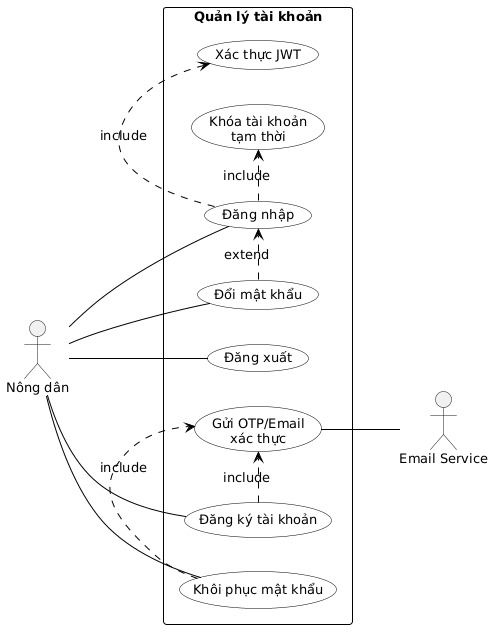
\includegraphics[width=\textwidth,height=0.38\textheight,keepaspectratio]{usecase-phanra-01-taikhoan.png}
    \caption{Biểu đồ Use Case phân rã: Quản lý tài khoản (Nông dân)}
    \label{fig:usecase-phanra-01-taikhoan}
\end{figure}

\begin{figure}[htbp]
    \centering
    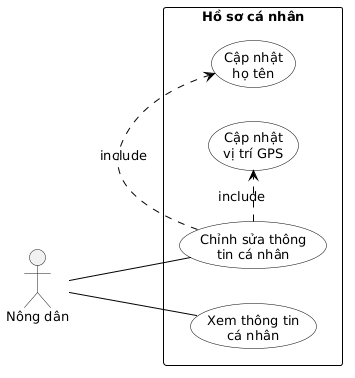
\includegraphics[width=\textwidth,height=0.38\textheight,keepaspectratio]{usecase-phanra-02-hosoca.png}
    \caption{Biểu đồ Use Case phân rã: Xem \& Chỉnh sửa hồ sơ cá nhân (Nông dân)}
    \label{fig:usecase-phanra-02-hosoca}
\end{figure}

\begin{figure}[htbp]
    \centering
    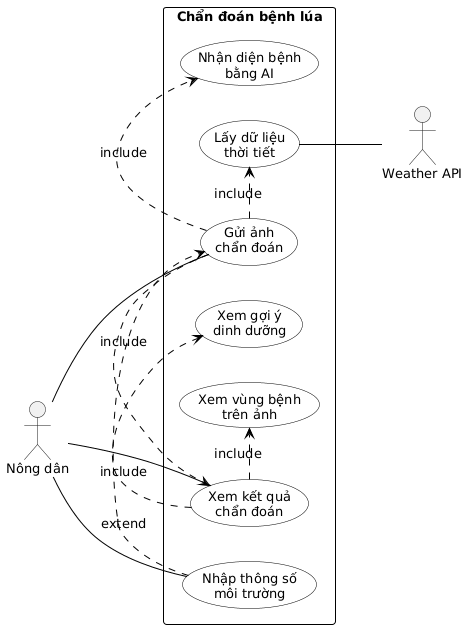
\includegraphics[width=\textwidth,height=0.38\textheight,keepaspectratio]{usecase-phanra-03-chandoan.png}
    \caption{Biểu đồ Use Case phân rã: Chẩn đoán bệnh lúa (Nông dân)}
    \label{fig:usecase-phanra-03-chandoan}
\end{figure}

\begin{figure}[htbp]
    \centering
    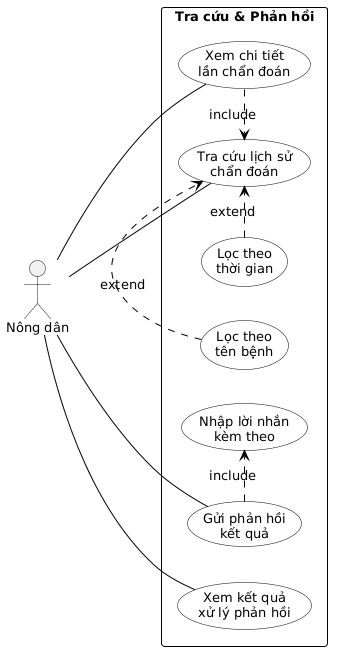
\includegraphics[width=\textwidth,height=0.38\textheight,keepaspectratio]{usecase-phanra-04-tracuu.png}
    \caption{Biểu đồ Use Case phân rã: Tra cứu lịch sử \& Gửi phản hồi (Nông dân)}
    \label{fig:usecase-phanra-04-tracuu}
\end{figure}

\clearpage

% --- Phân rã Quản trị viên (AD) ---
\subsubsection{Các Use Case của Quản trị viên (AD)}

\begin{figure}[htbp]
    \centering
    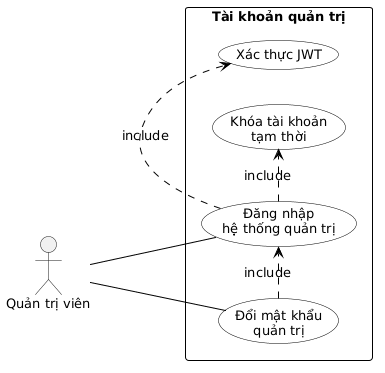
\includegraphics[width=\textwidth,height=0.38\textheight,keepaspectratio]{usecase-phanra-ad01-taikhoan.png}
    \caption{Biểu đồ Use Case phân rã: Quản lý tài khoản (Quản trị viên)}
    \label{fig:usecase-phanra-ad01-taikhoan}
\end{figure}

\begin{figure}[htbp]
    \centering
    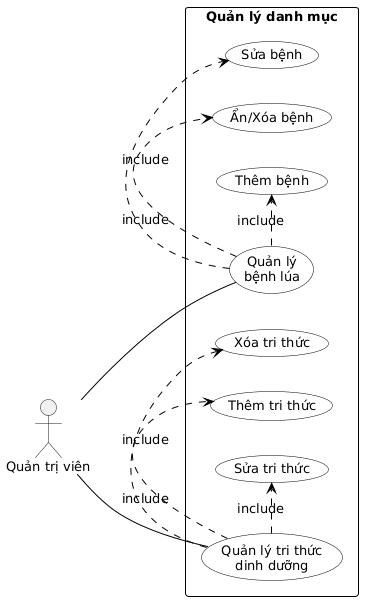
\includegraphics[width=\textwidth,height=0.38\textheight,keepaspectratio]{usecase-phanra-ad02-danhmuc.png}
    \caption{Biểu đồ Use Case phân rã: Quản lý danh mục bệnh lúa (Quản trị viên)}
    \label{fig:usecase-phanra-ad02-danhmuc}
\end{figure}

\begin{figure}[htbp]
    \centering
    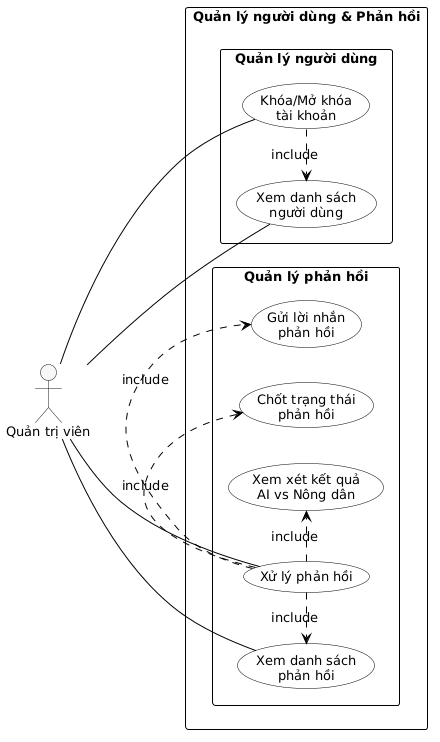
\includegraphics[width=\textwidth,height=0.38\textheight,keepaspectratio]{usecase-phanra-ad03-nguoidung.png}
    \caption{Biểu đồ Use Case phân rã: Quản lý người dùng \& phản hồi (Quản trị viên)}
    \label{fig:usecase-phanra-ad03-nguoidung}
\end{figure}

\begin{figure}[htbp]
    \centering
    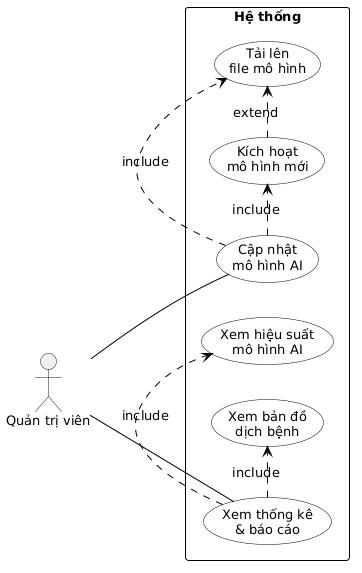
\includegraphics[width=\textwidth,height=0.38\textheight,keepaspectratio]{usecase-phanra-ad04-hethong.png}
    \caption{Biểu đồ Use Case phân rã: Quản lý hệ thống (Quản trị viên)}
    \label{fig:usecase-phanra-ad04-hethong}
\end{figure}

\hrulefill

% ============================================================
\section{Biểu đồ tuần tự (Sequence Diagrams)}

\subsection{SD-01: Đăng ký tài khoản (có xác thực email)}
% \noindent\textit{[Chèn ảnh SD-01 tại đây]}
\begin{figure}[htbp]
    \centering
    \includegraphics[width=\textwidth,height=0.85\textheight,keepaspectratio]{sd-01-register.png}
    \caption{Biểu đồ tuần tự: Đăng ký tài khoản}
    \label{fig:sd-01}
\end{figure}

\subsection{SD-02: Đăng nhập hệ thống}
% \noindent\textit{[Chèn ảnh SD-02 tại đây]}
\begin{figure}[htbp]
    \centering
    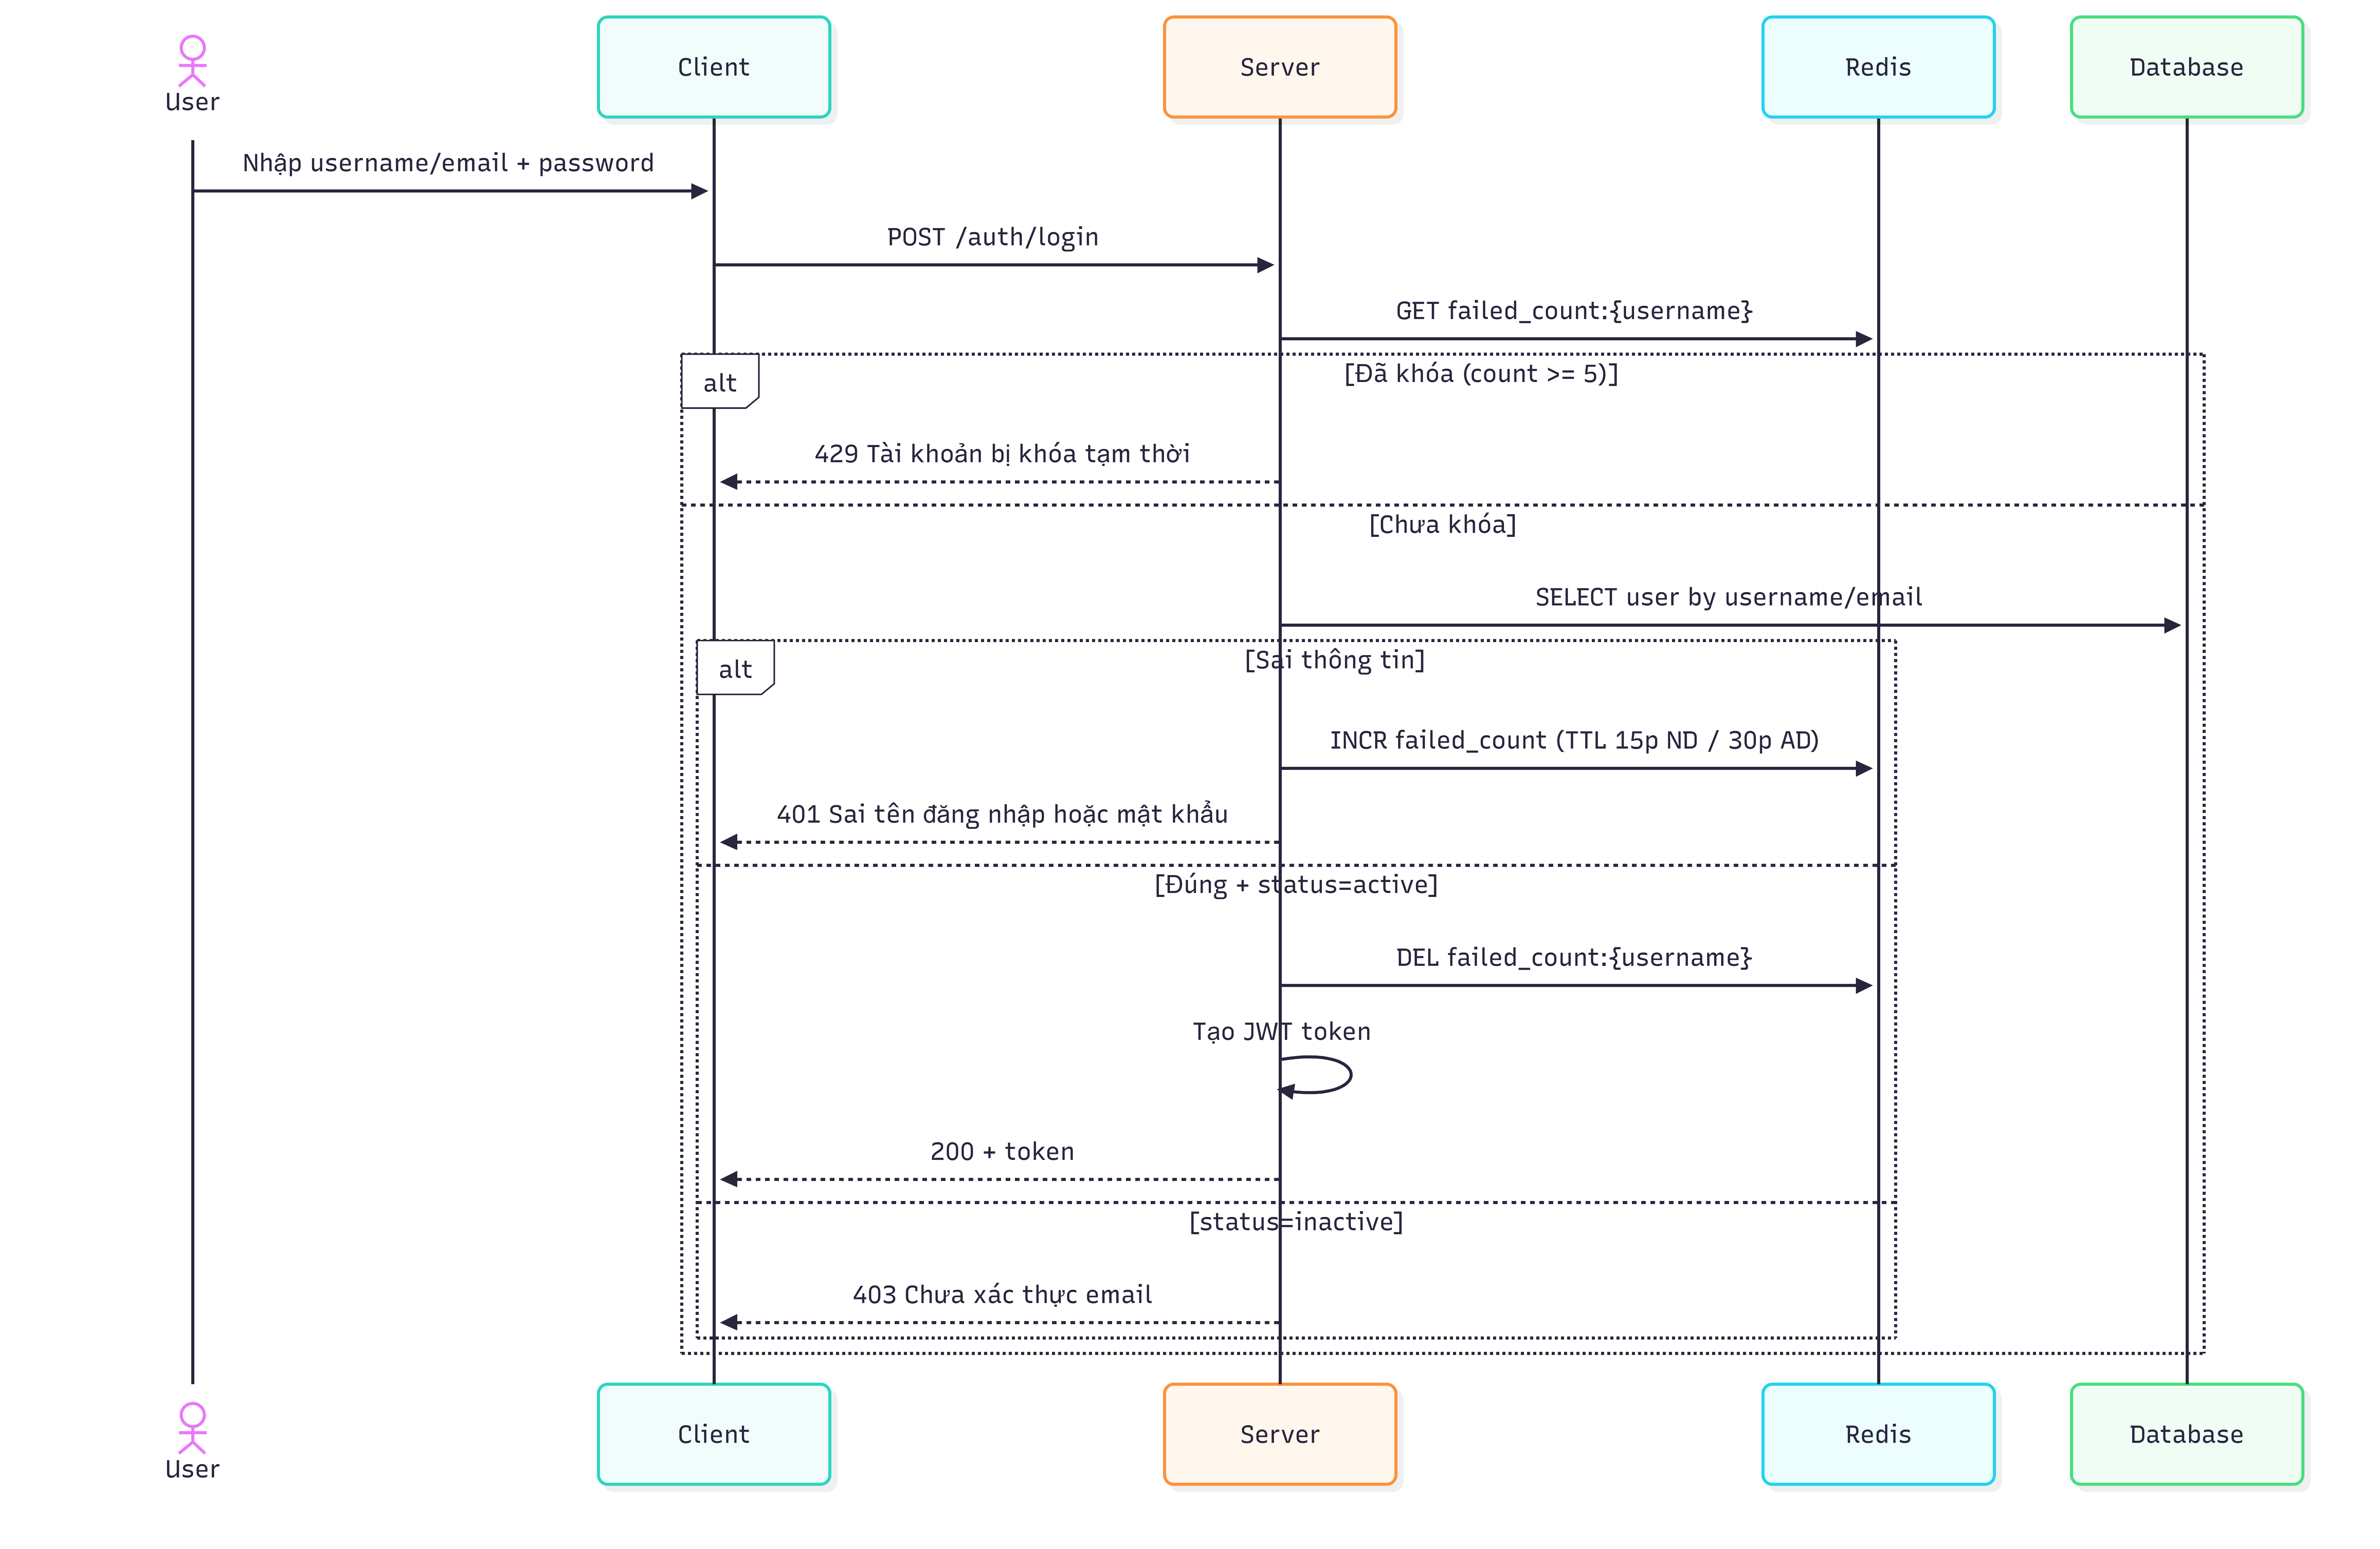
\includegraphics[width=\textwidth,height=0.85\textheight,keepaspectratio]{sd-02-login.png}
    \caption{Biểu đồ tuần tự: Đăng nhập hệ thống}
    \label{fig:sd-02}
\end{figure}

\subsection{SD-03: Khôi phục mật khẩu}
% \noindent\textit{[Chèn ảnh SD-03 tại đây]}
\begin{figure}[htbp]
    \centering
    \includegraphics[width=\textwidth,height=0.85\textheight,keepaspectratio]{sd-03-forgot-password.png}
    \caption{Biểu đồ tuần tự: Khôi phục mật khẩu}
    \label{fig:sd-03}
\end{figure}

\subsection{SD-04: Xem \& Chỉnh sửa hồ sơ cá nhân}
% \noindent\textit{[Chèn ảnh SD-04 tại đây]}
\begin{figure}[htbp]
    \centering
    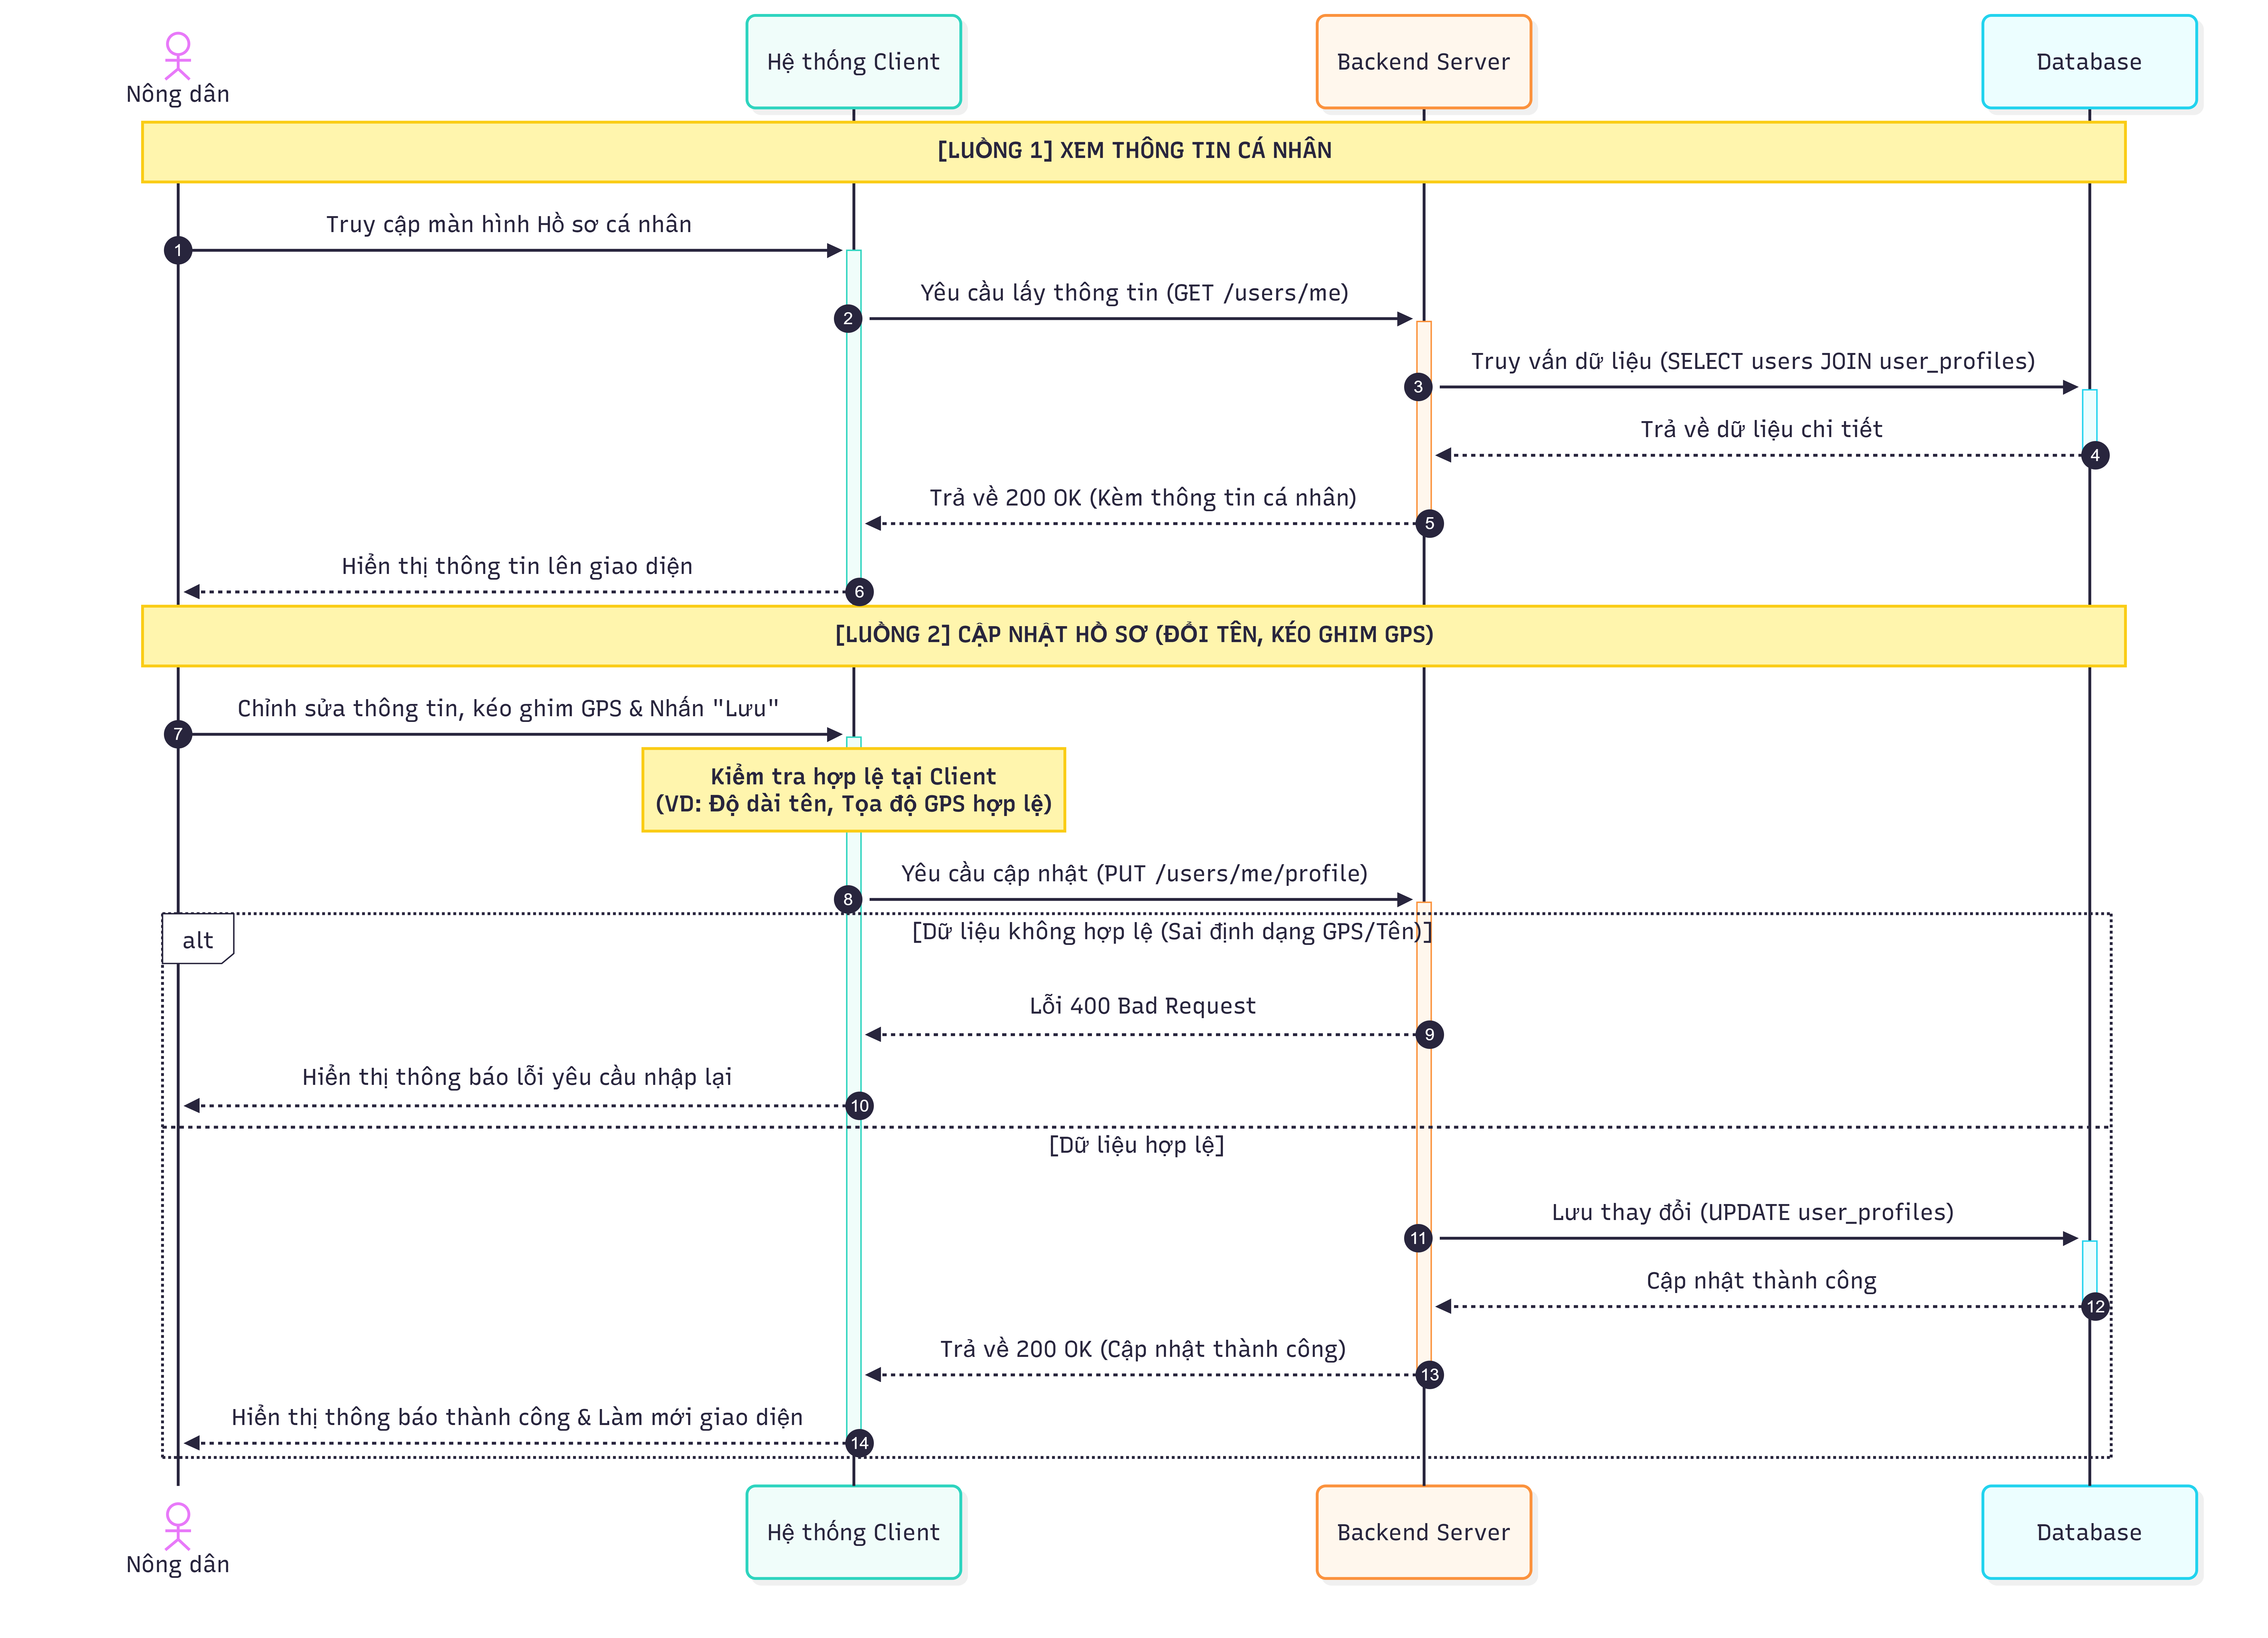
\includegraphics[width=\textwidth,height=0.85\textheight,keepaspectratio]{sd-04-profile.png}
    \caption{Biểu đồ tuần tự: Xem và chỉnh sửa hồ sơ cá nhân}
    \label{fig:sd-04}
\end{figure}

\subsection{SD-05: Gửi ảnh chẩn đoán (Core Flow)}
% \noindent\textit{[Chèn ảnh SD-05 tại đây]}
\begin{figure}[htbp]
    \centering
    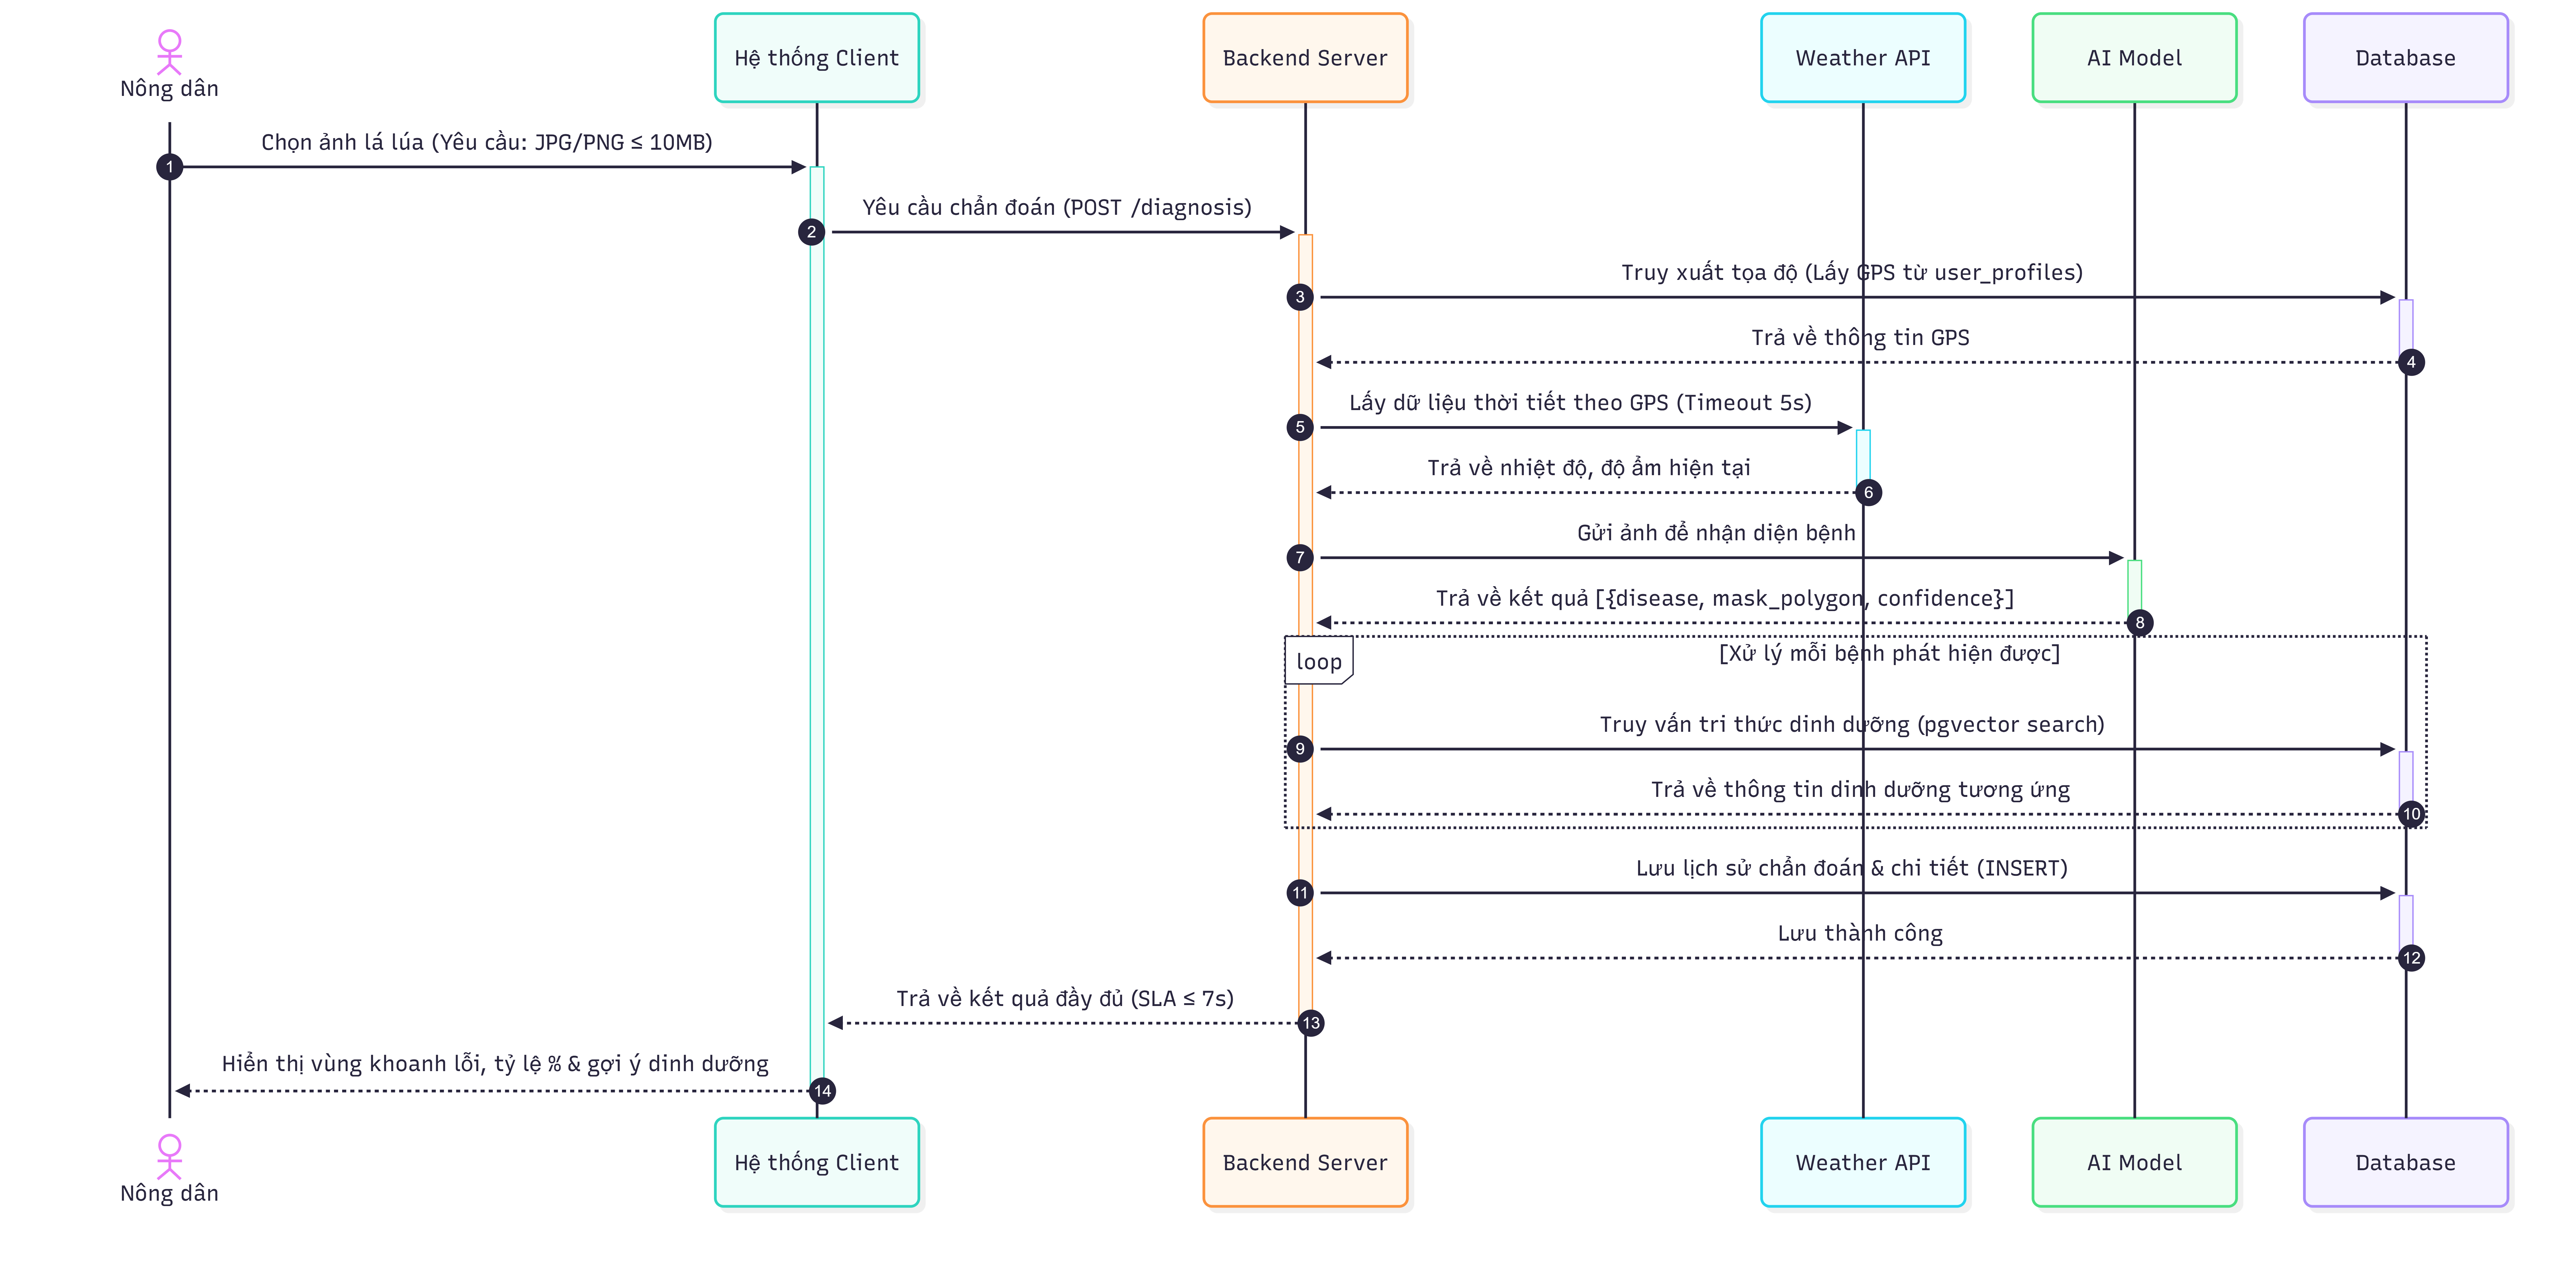
\includegraphics[width=\textwidth,height=0.85\textheight,keepaspectratio]{sd-05-diagnosis.png}
    \caption{Biểu đồ tuần tự: Gửi ảnh chẩn đoán}
    \label{fig:sd-05}
\end{figure}

\subsection{SD-06: Nhập thông số môi trường bổ sung}
% \noindent\textit{[Chèn ảnh SD-06 tại đây]}
\begin{figure}[htbp]
    \centering
    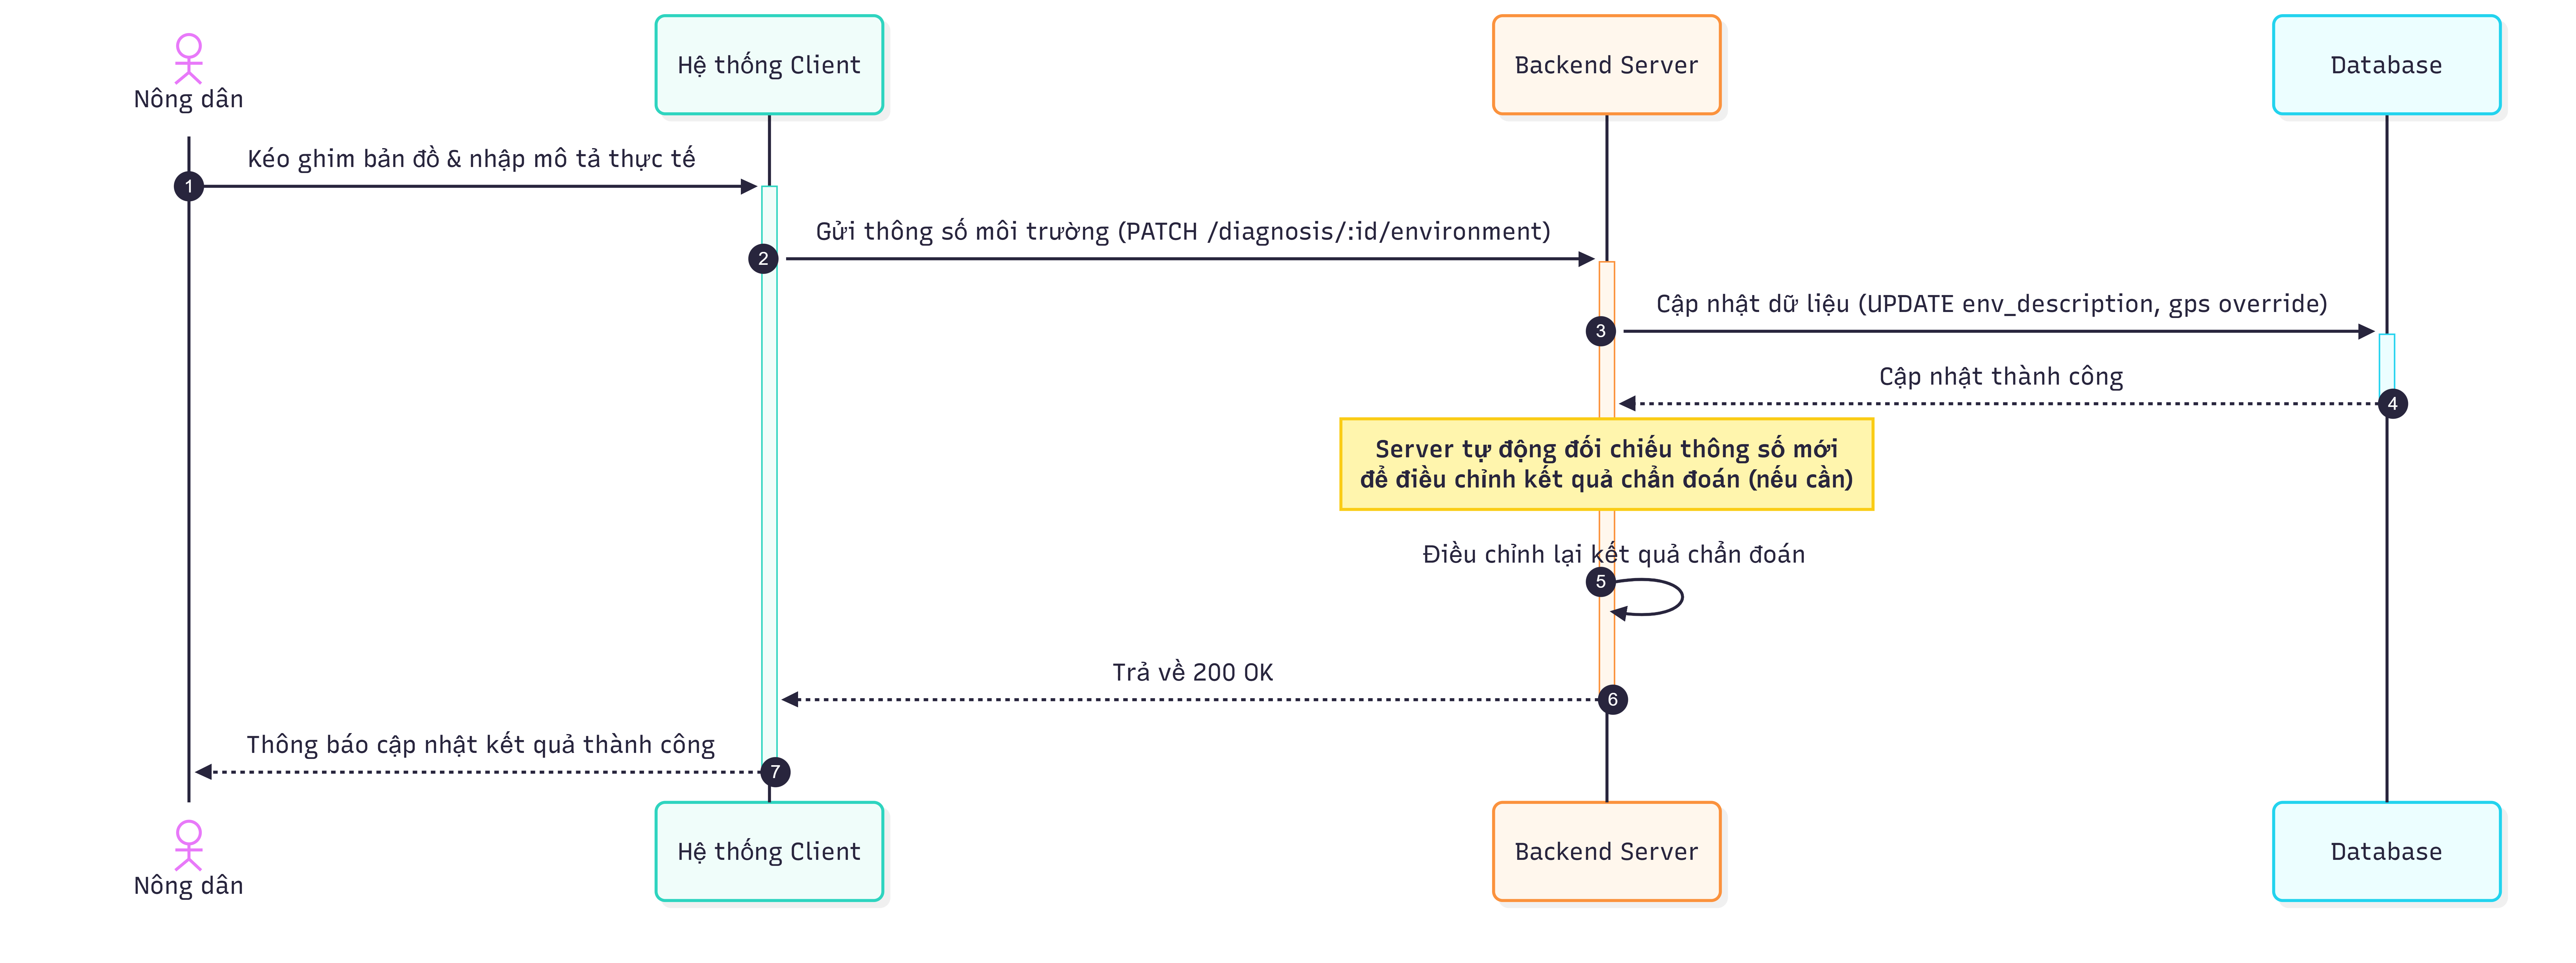
\includegraphics[width=\textwidth,height=0.85\textheight,keepaspectratio]{sd-06-environment.png}
    \caption{Biểu đồ tuần tự: Nhập thông số môi trường bổ sung}
    \label{fig:sd-06}
\end{figure}

\subsection{SD-07: Tra cứu lịch sử \& Xem chi tiết}
% \noindent\textit{[Chèn ảnh SD-07 tại đây]}
\begin{figure}[htbp]
    \centering
    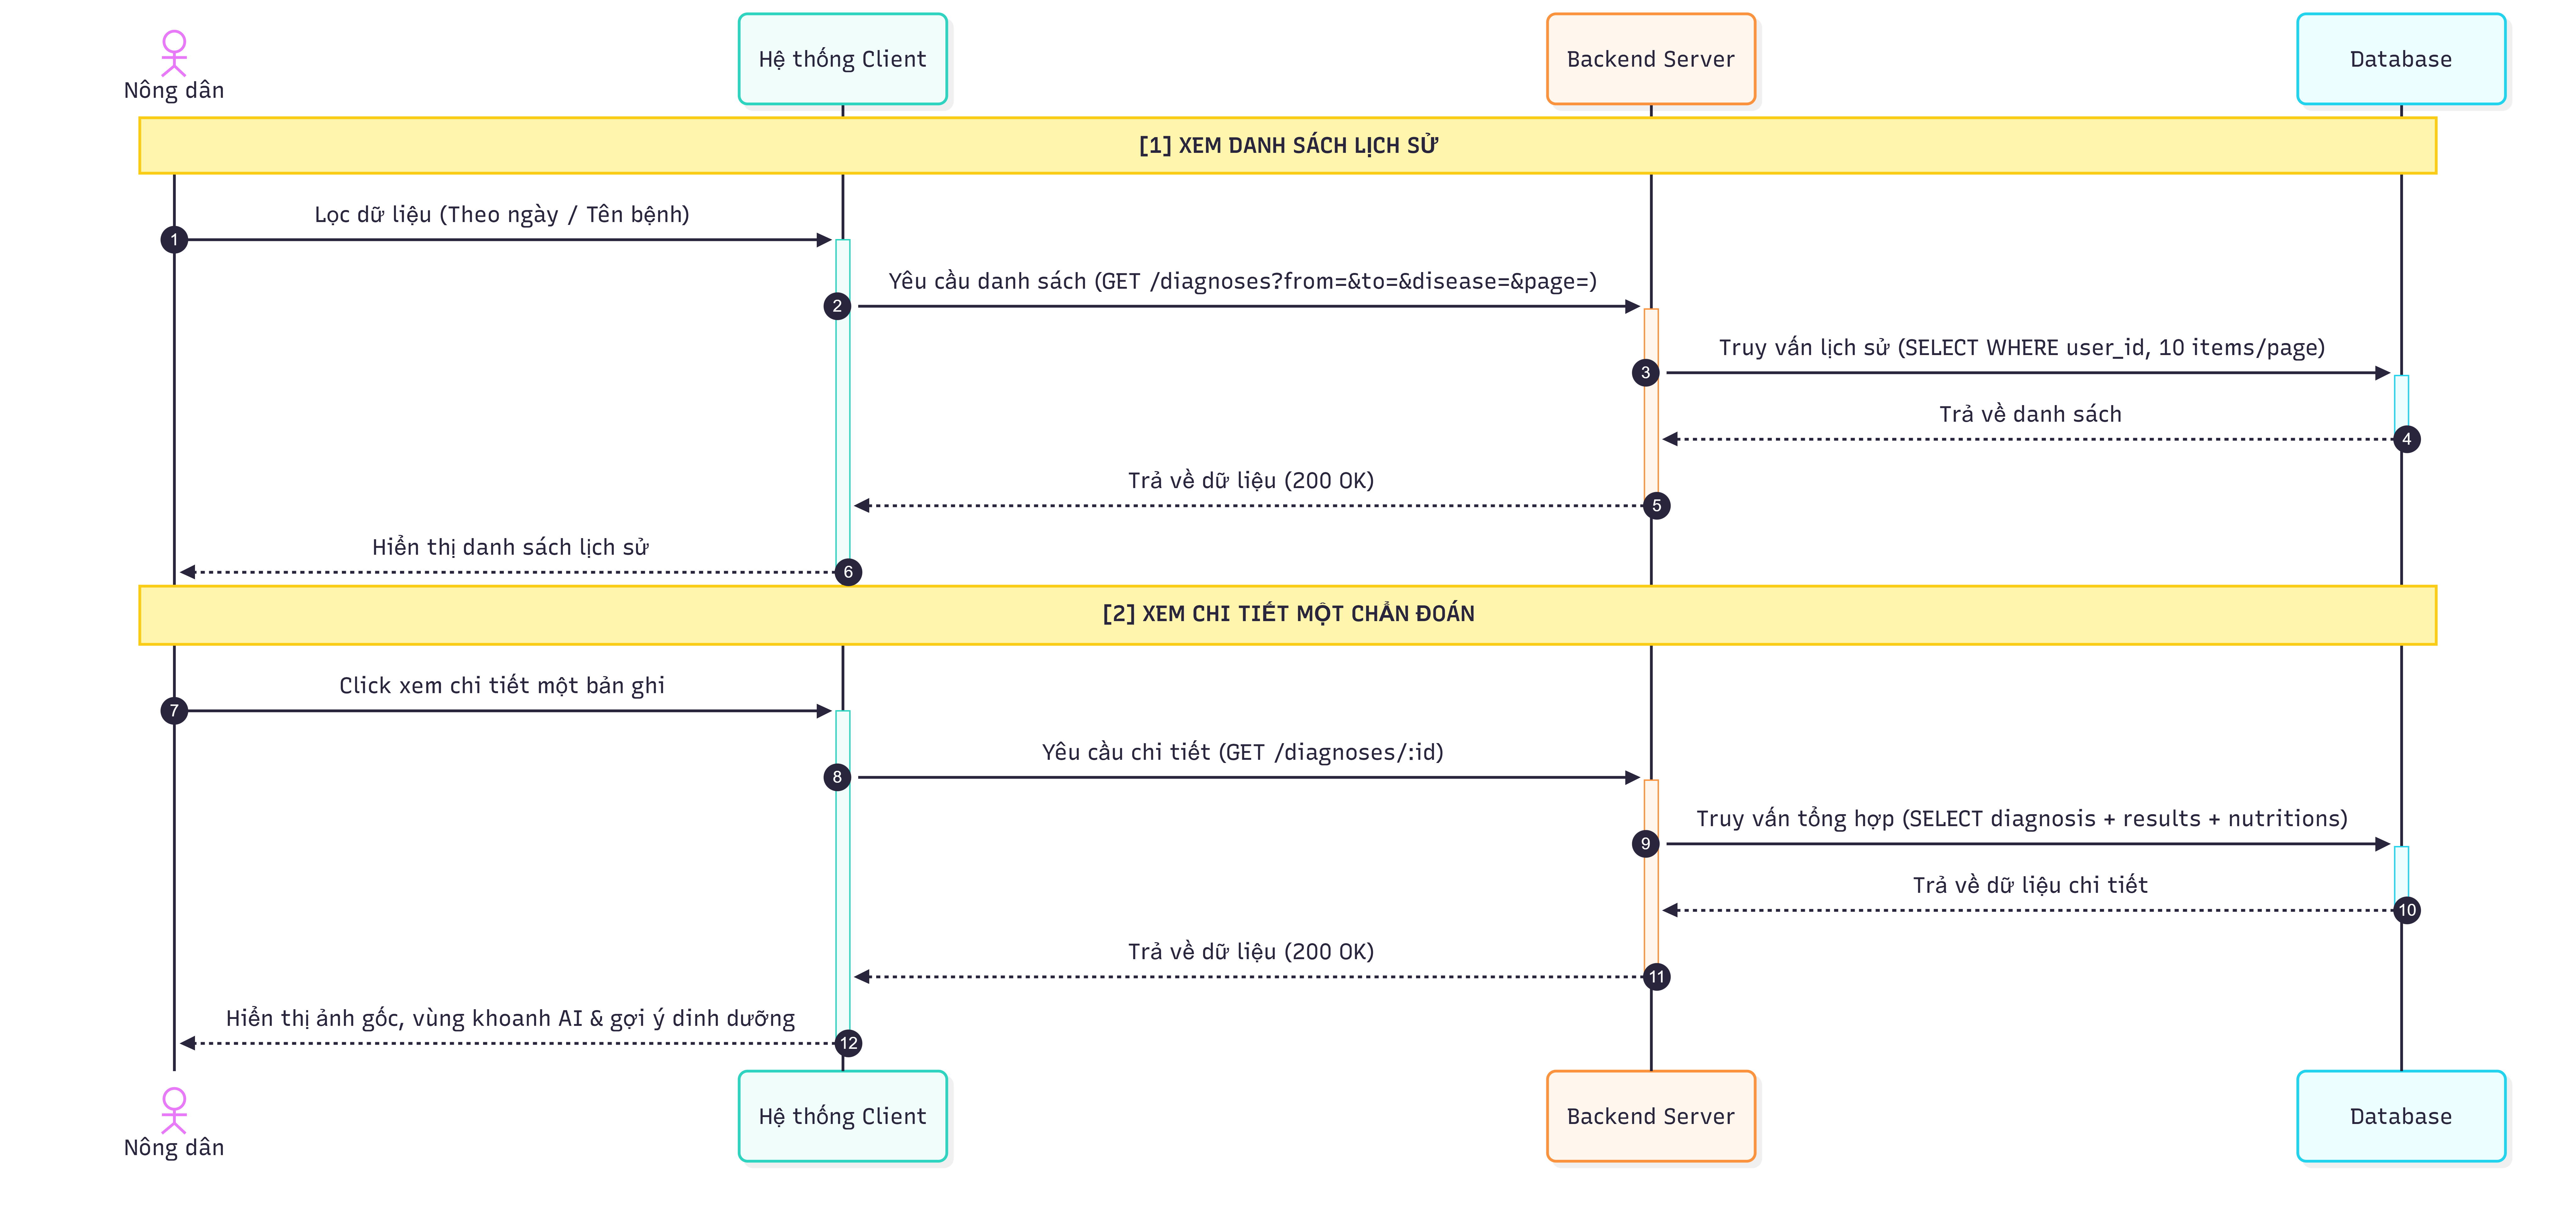
\includegraphics[width=\textwidth,height=0.85\textheight,keepaspectratio]{sd-07-history.png}
    \caption{Biểu đồ tuần tự: Tra cứu lịch sử và xem chi tiết}
    \label{fig:sd-07}
\end{figure}

\subsection{SD-08: Gửi phản hồi kết quả \& SD-09: Xem kết quả xử lý phản hồi}
% \noindent\textit{[Chèn ảnh SD-08, SD-09 tại đây]}
\begin{figure}[htbp]
    \centering
    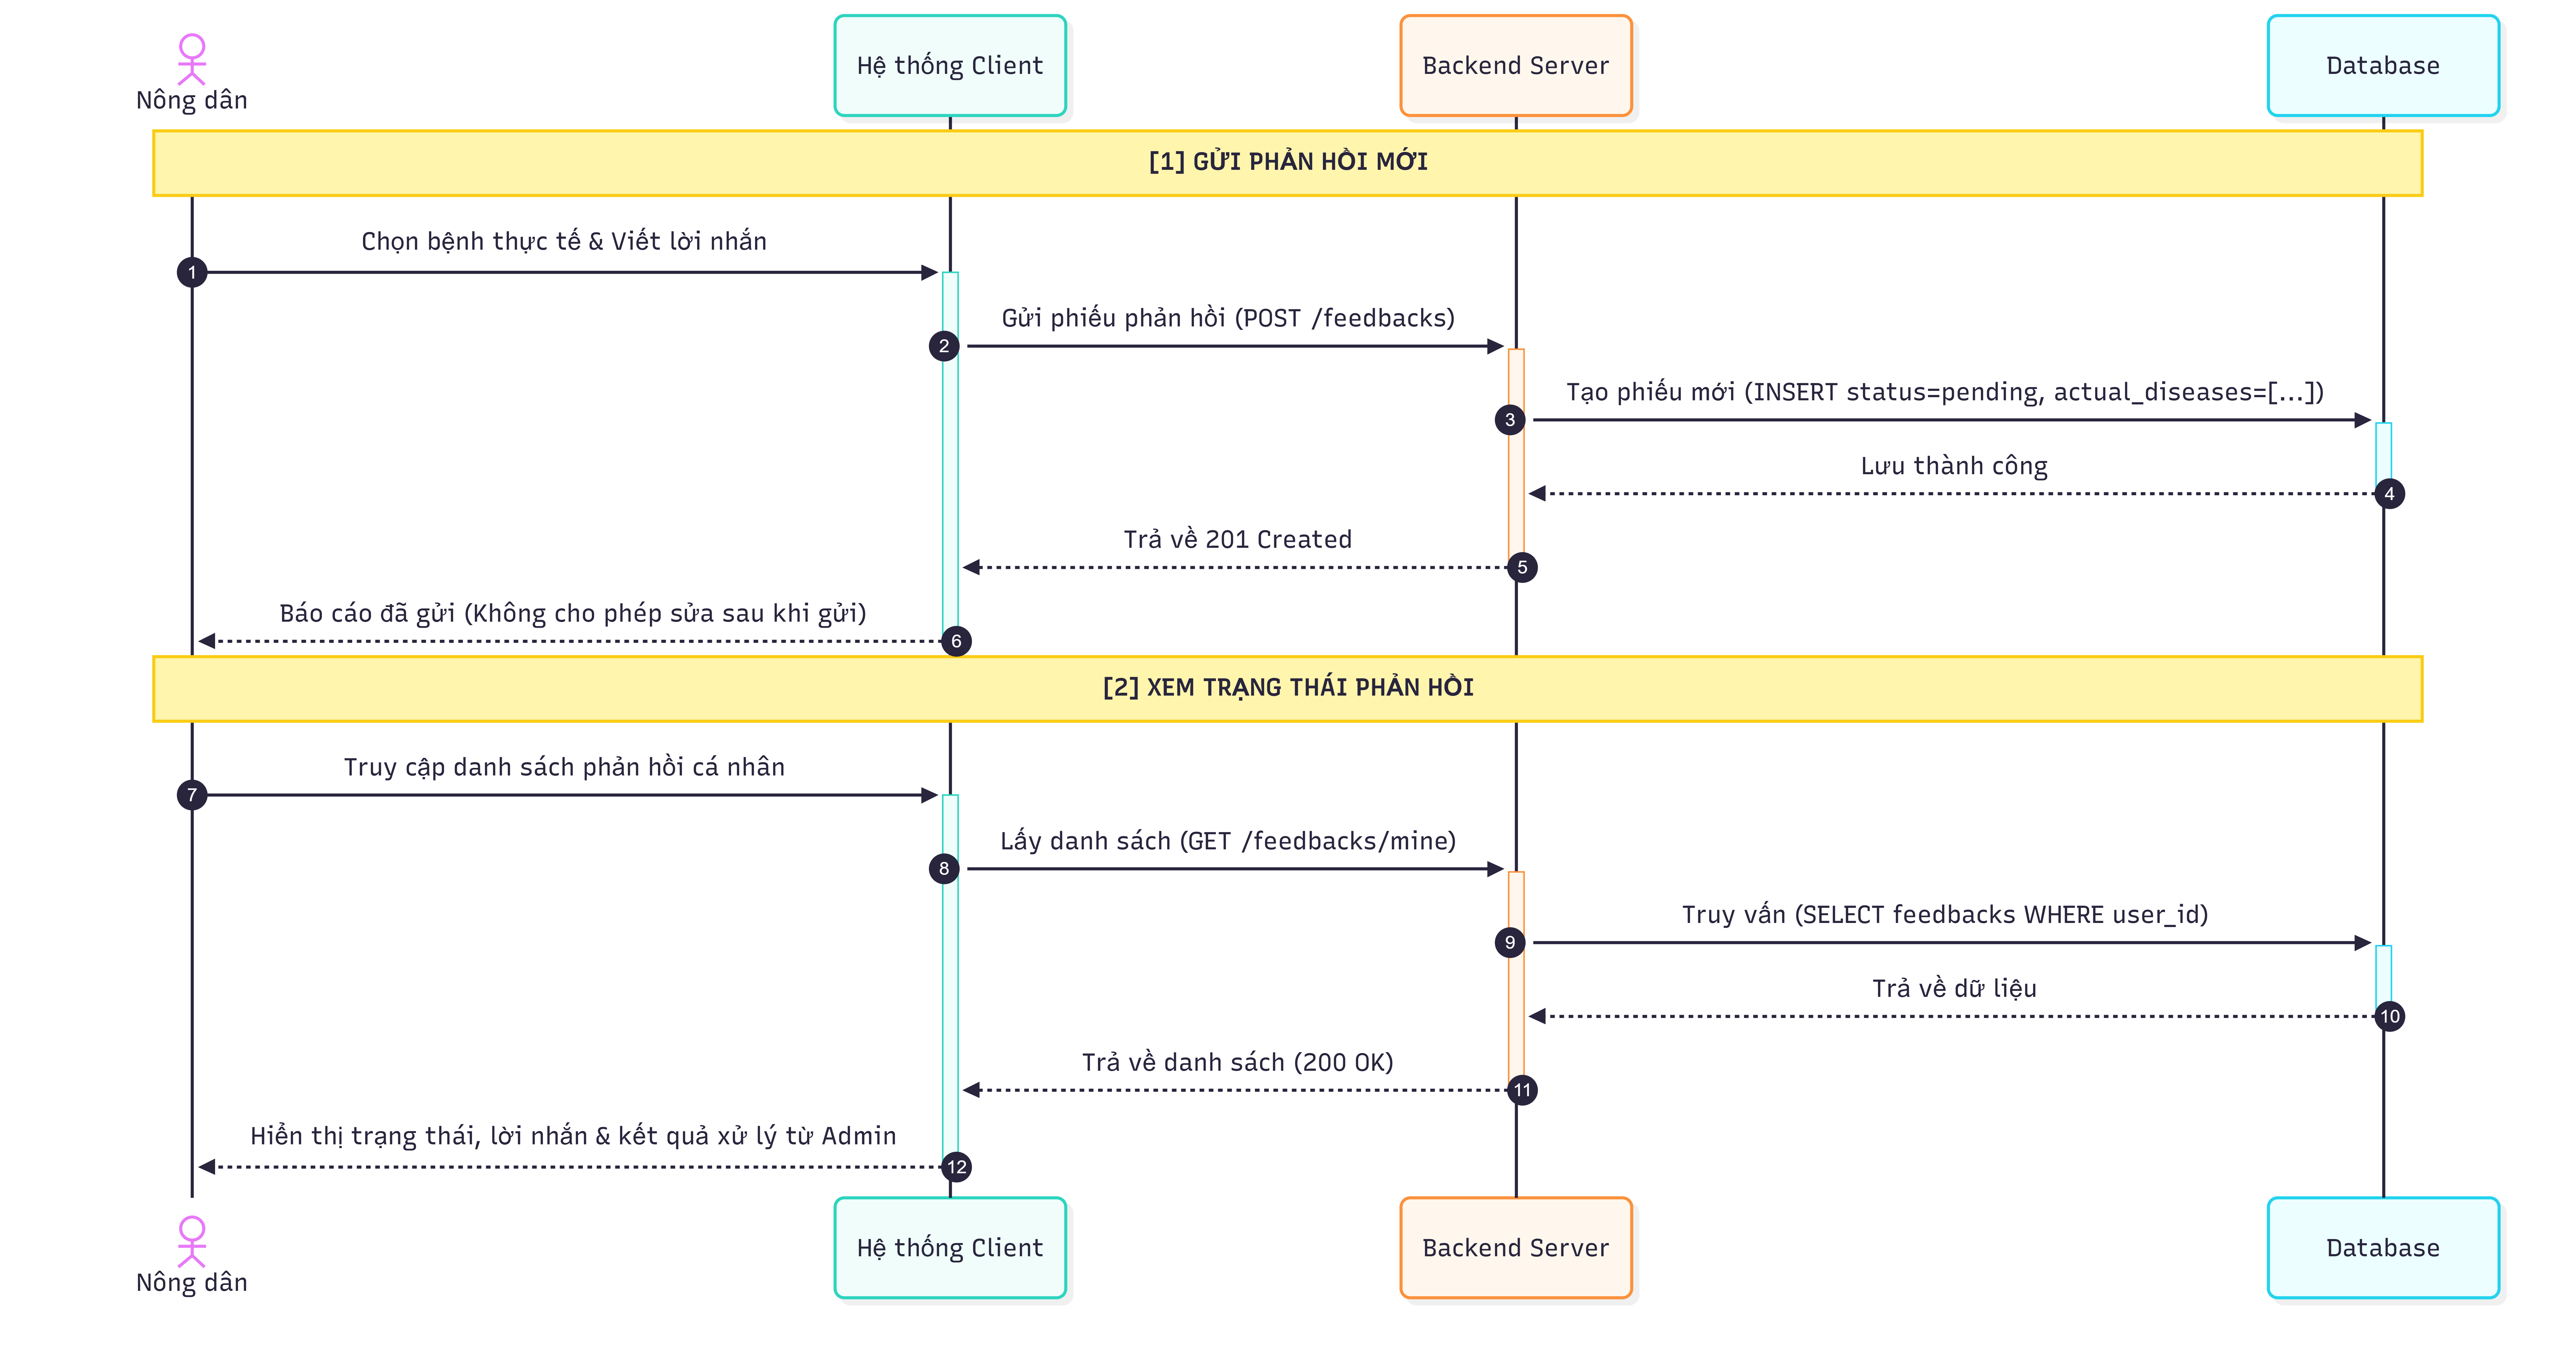
\includegraphics[width=\textwidth,height=0.85\textheight,keepaspectratio]{sd-0809-feedback.png}
    \caption{Biểu đồ tuần tự: Gửi phản hồi và xem kết quả xử lý}
    \label{fig:sd-0809}
\end{figure}

\subsection{SD-10: Quản lý bệnh lúa (CRUD)}
% \noindent\textit{[Chèn ảnh SD-10 tại đây]}
\begin{figure}[htbp]
    \centering
    \includegraphics[width=\textwidth,height=0.85\textheight,keepaspectratio]{sd-10-disease-crud.png}
    \caption{Biểu đồ tuần tự: Quản lý bệnh lúa (CRUD)}
    \label{fig:sd-10}
\end{figure}

\subsection{SD-11: Quản lý tri thức dinh dưỡng}
% \noindent\textit{[Chèn ảnh SD-11 tại đây]}
\begin{figure}[htbp]
    \centering
    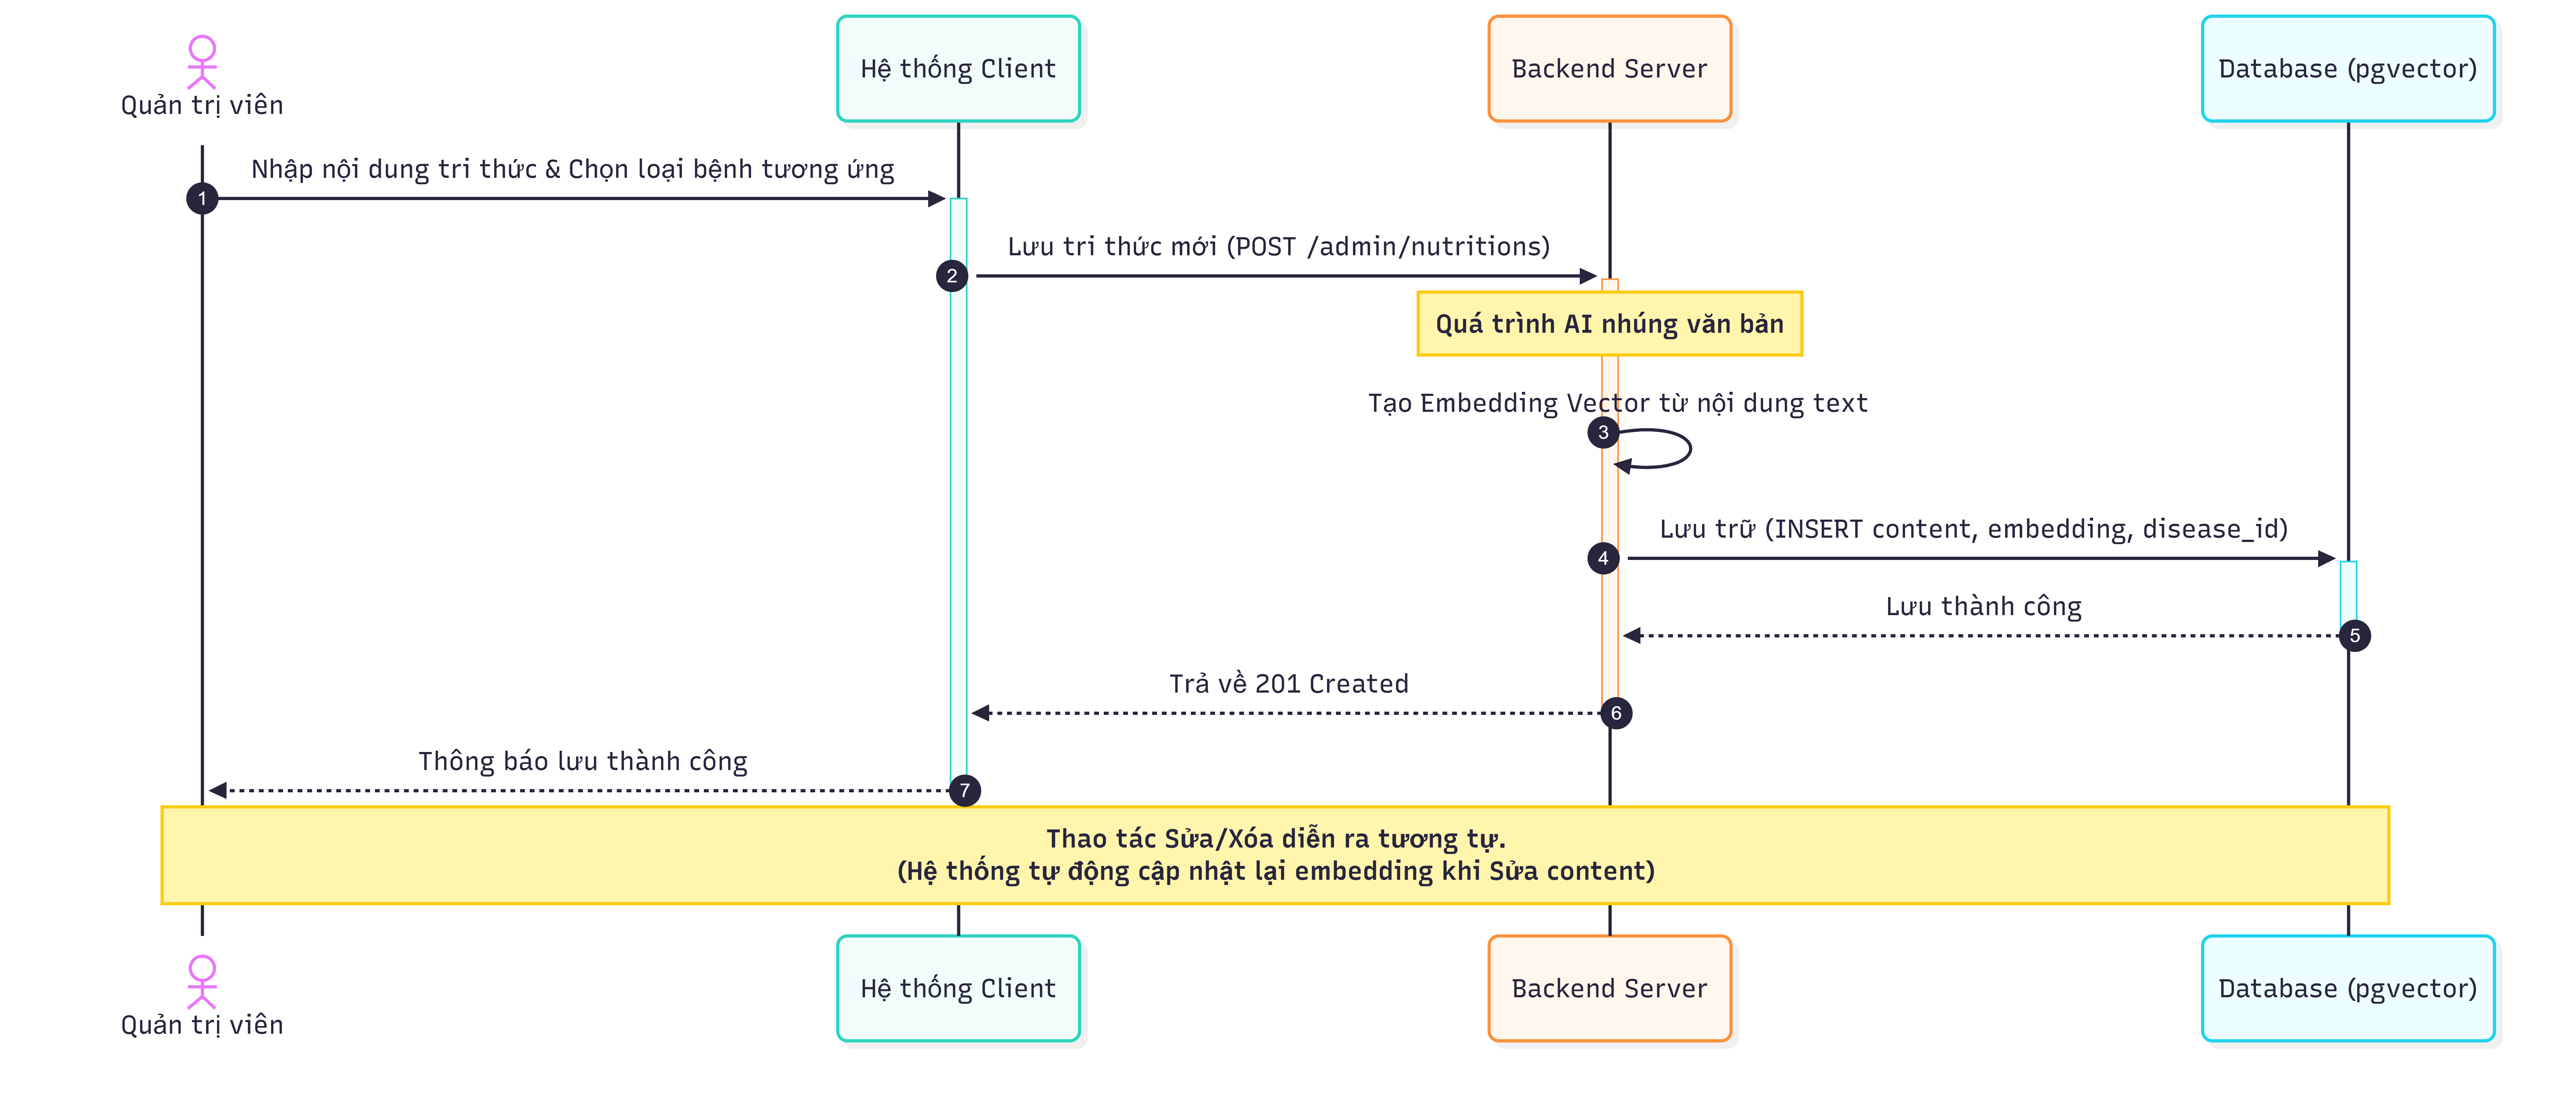
\includegraphics[width=\textwidth,height=0.85\textheight,keepaspectratio]{sd-11-nutrition.png}
    \caption{Biểu đồ tuần tự: Quản lý tri thức dinh dưỡng}
    \label{fig:sd-11}
\end{figure}

\subsection{SD-12: Quản lý người dùng}
% \noindent\textit{[Chèn ảnh SD-12 tại đây]}
\begin{figure}[htbp]
    \centering
    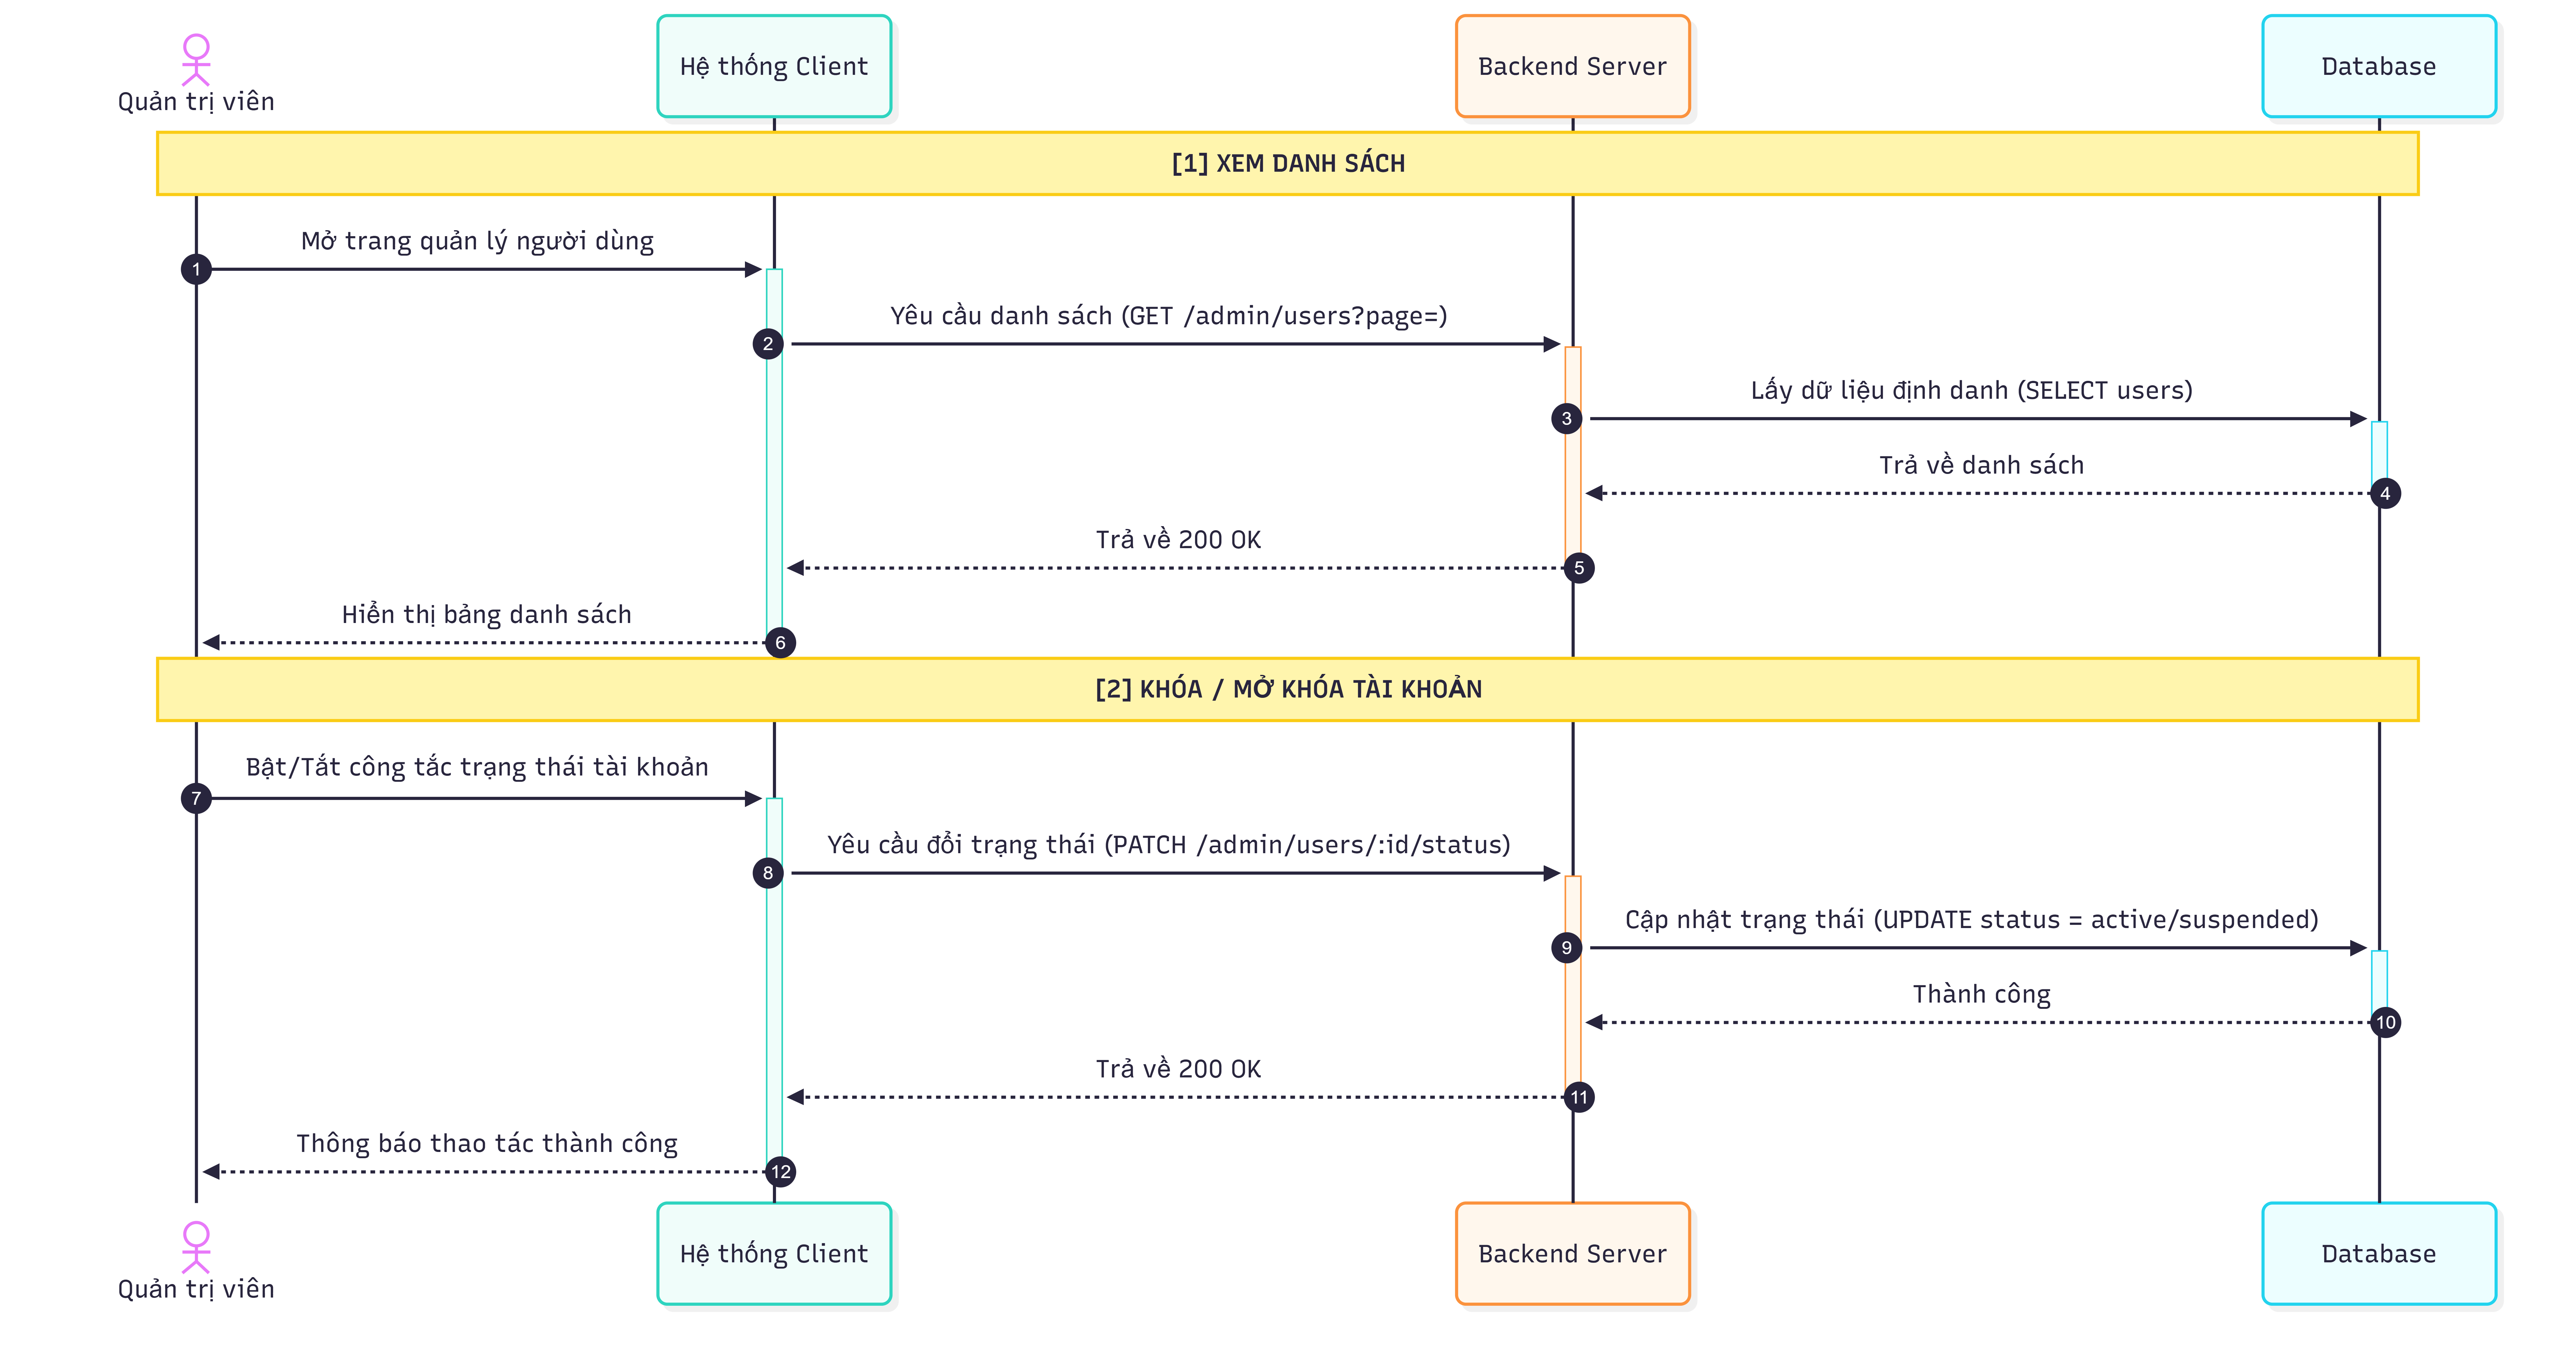
\includegraphics[width=\textwidth,height=0.85\textheight,keepaspectratio]{sd-12-user-management.png}
    \caption{Biểu đồ tuần tự: Quản lý người dùng}
    \label{fig:sd-12}
\end{figure}

\subsection{SD-13: Xử lý phản hồi (Admin)}
% \noindent\textit{[Chèn ảnh SD-13 tại đây]}
\begin{figure}[htbp]
    \centering
    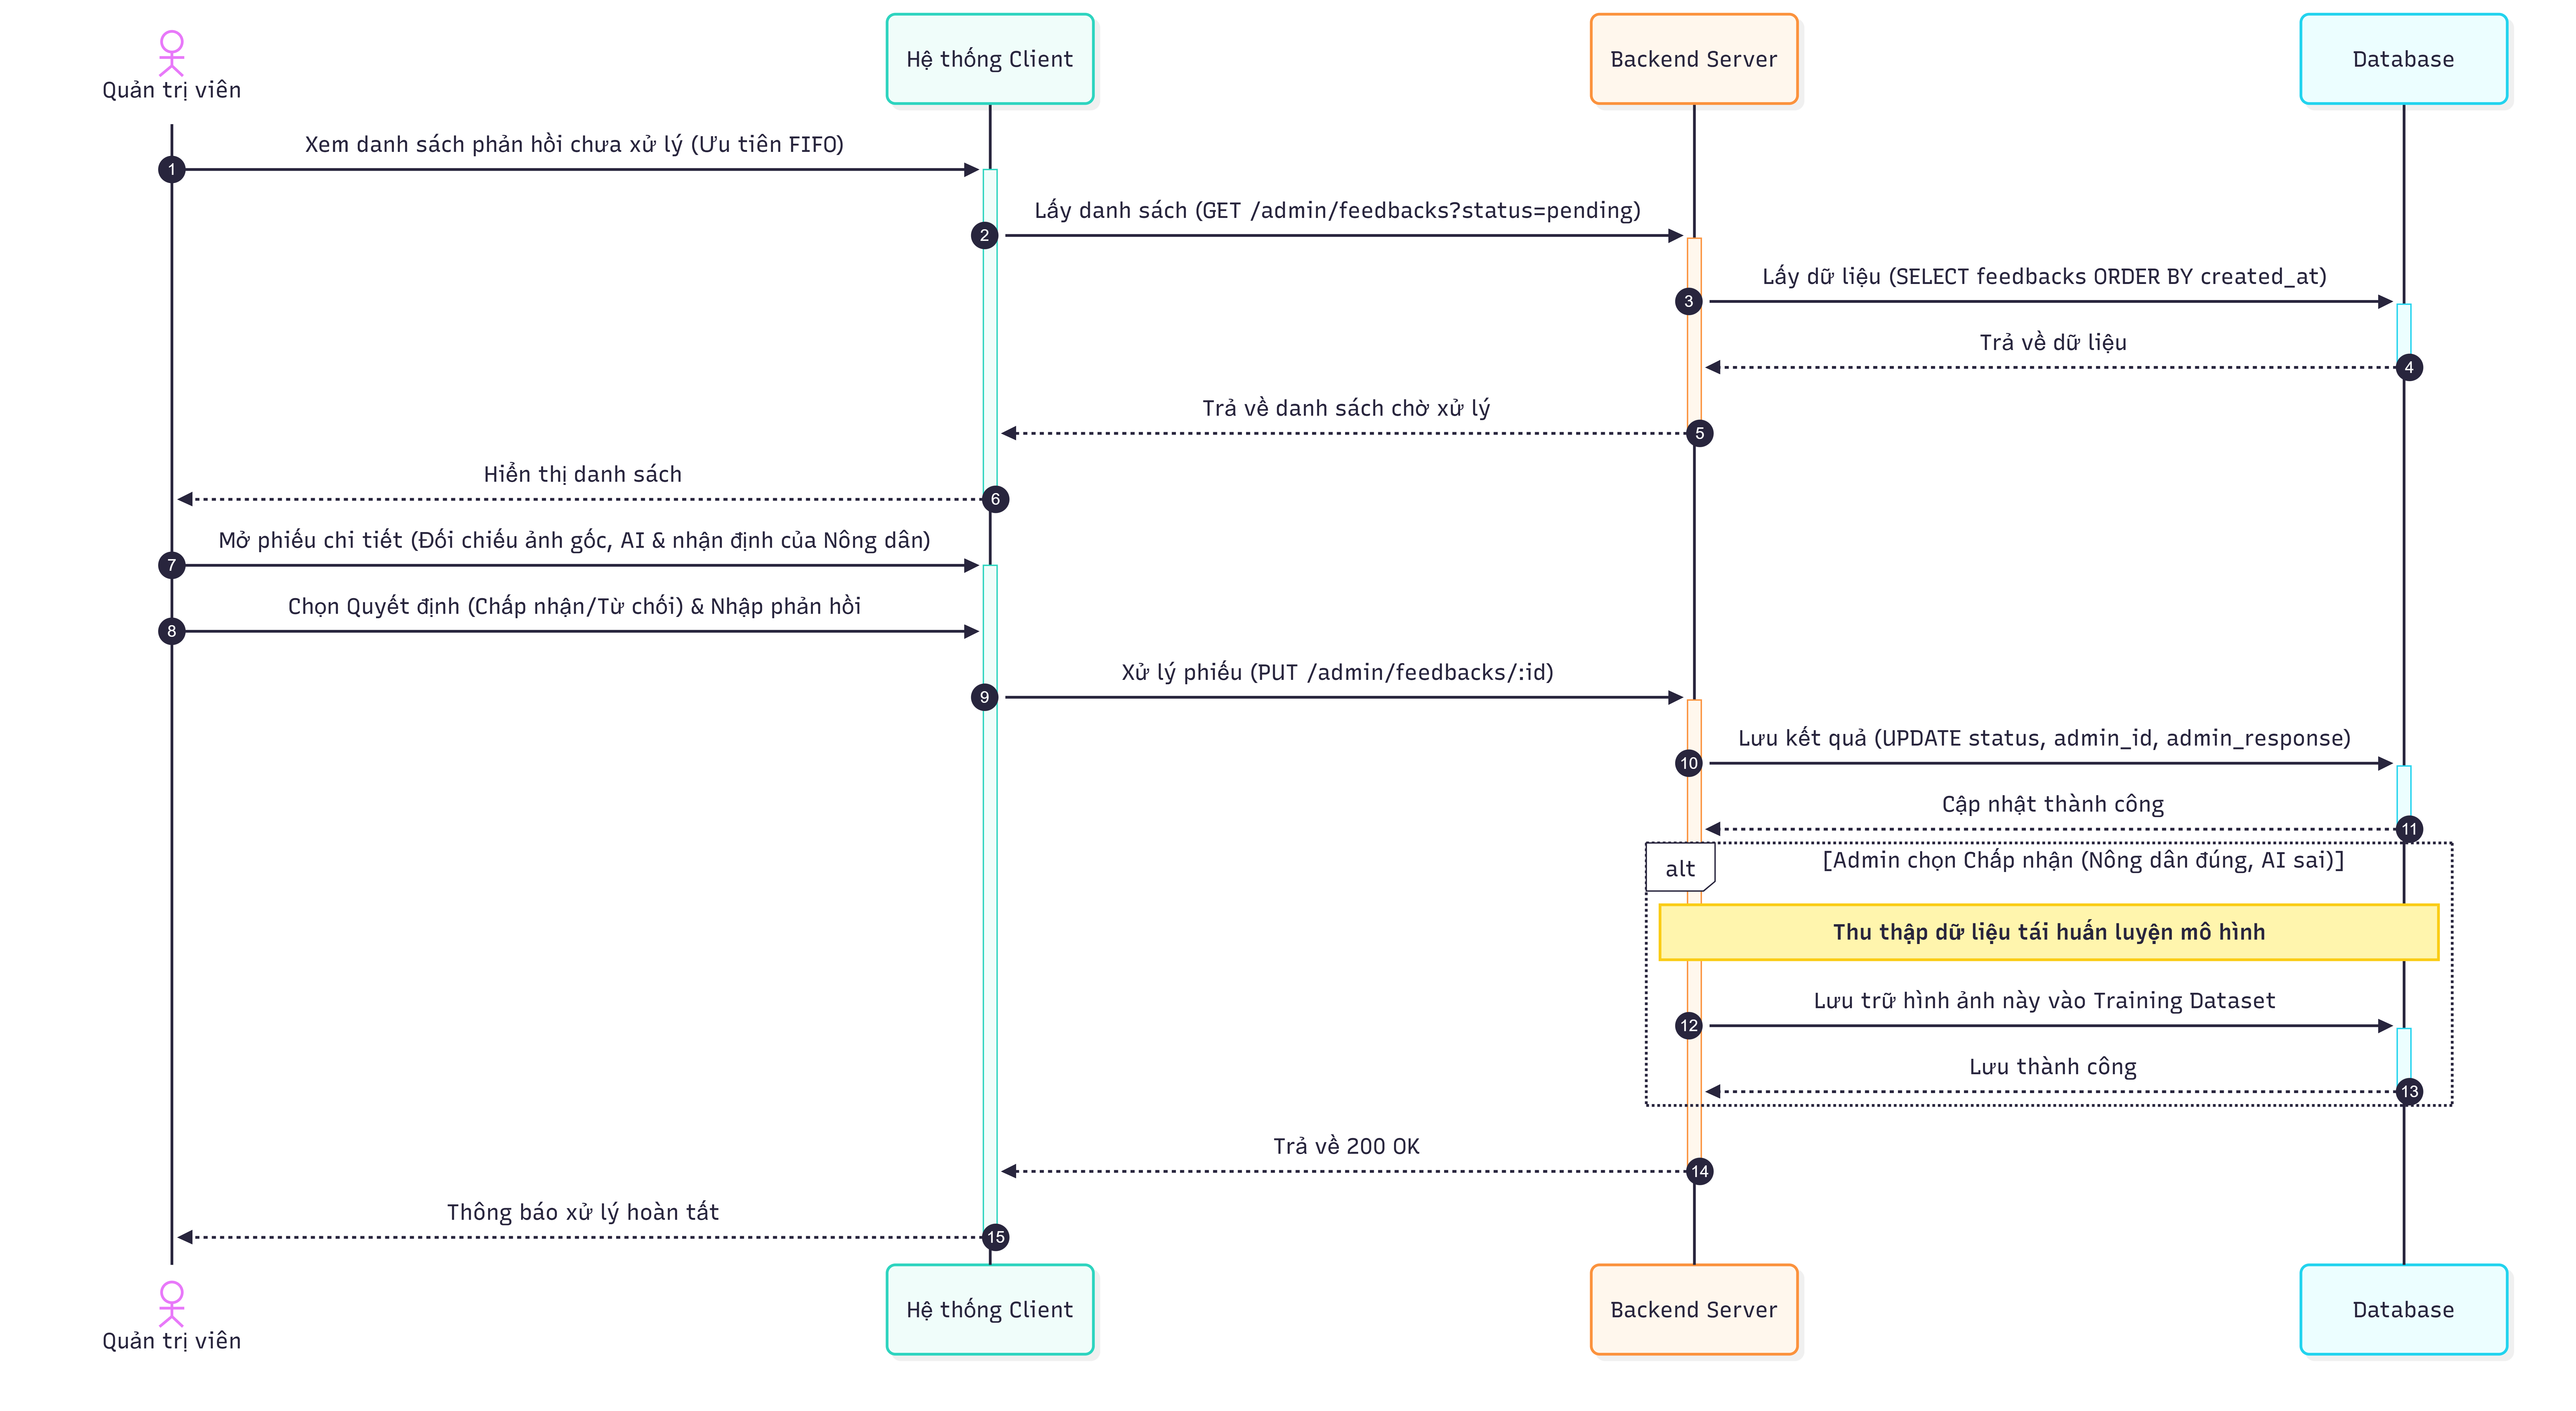
\includegraphics[width=\textwidth,height=0.85\textheight,keepaspectratio]{sd-13-feedback-admin.png}
    \caption{Biểu đồ tuần tự: Xử lý phản hồi (Admin)}
    \label{fig:sd-13}
\end{figure}

\subsection{SD-14: Cập nhật mô hình AI}
% \noindent\textit{[Chèn ảnh SD-14 tại đây]}
\begin{figure}[htbp]
    \centering
    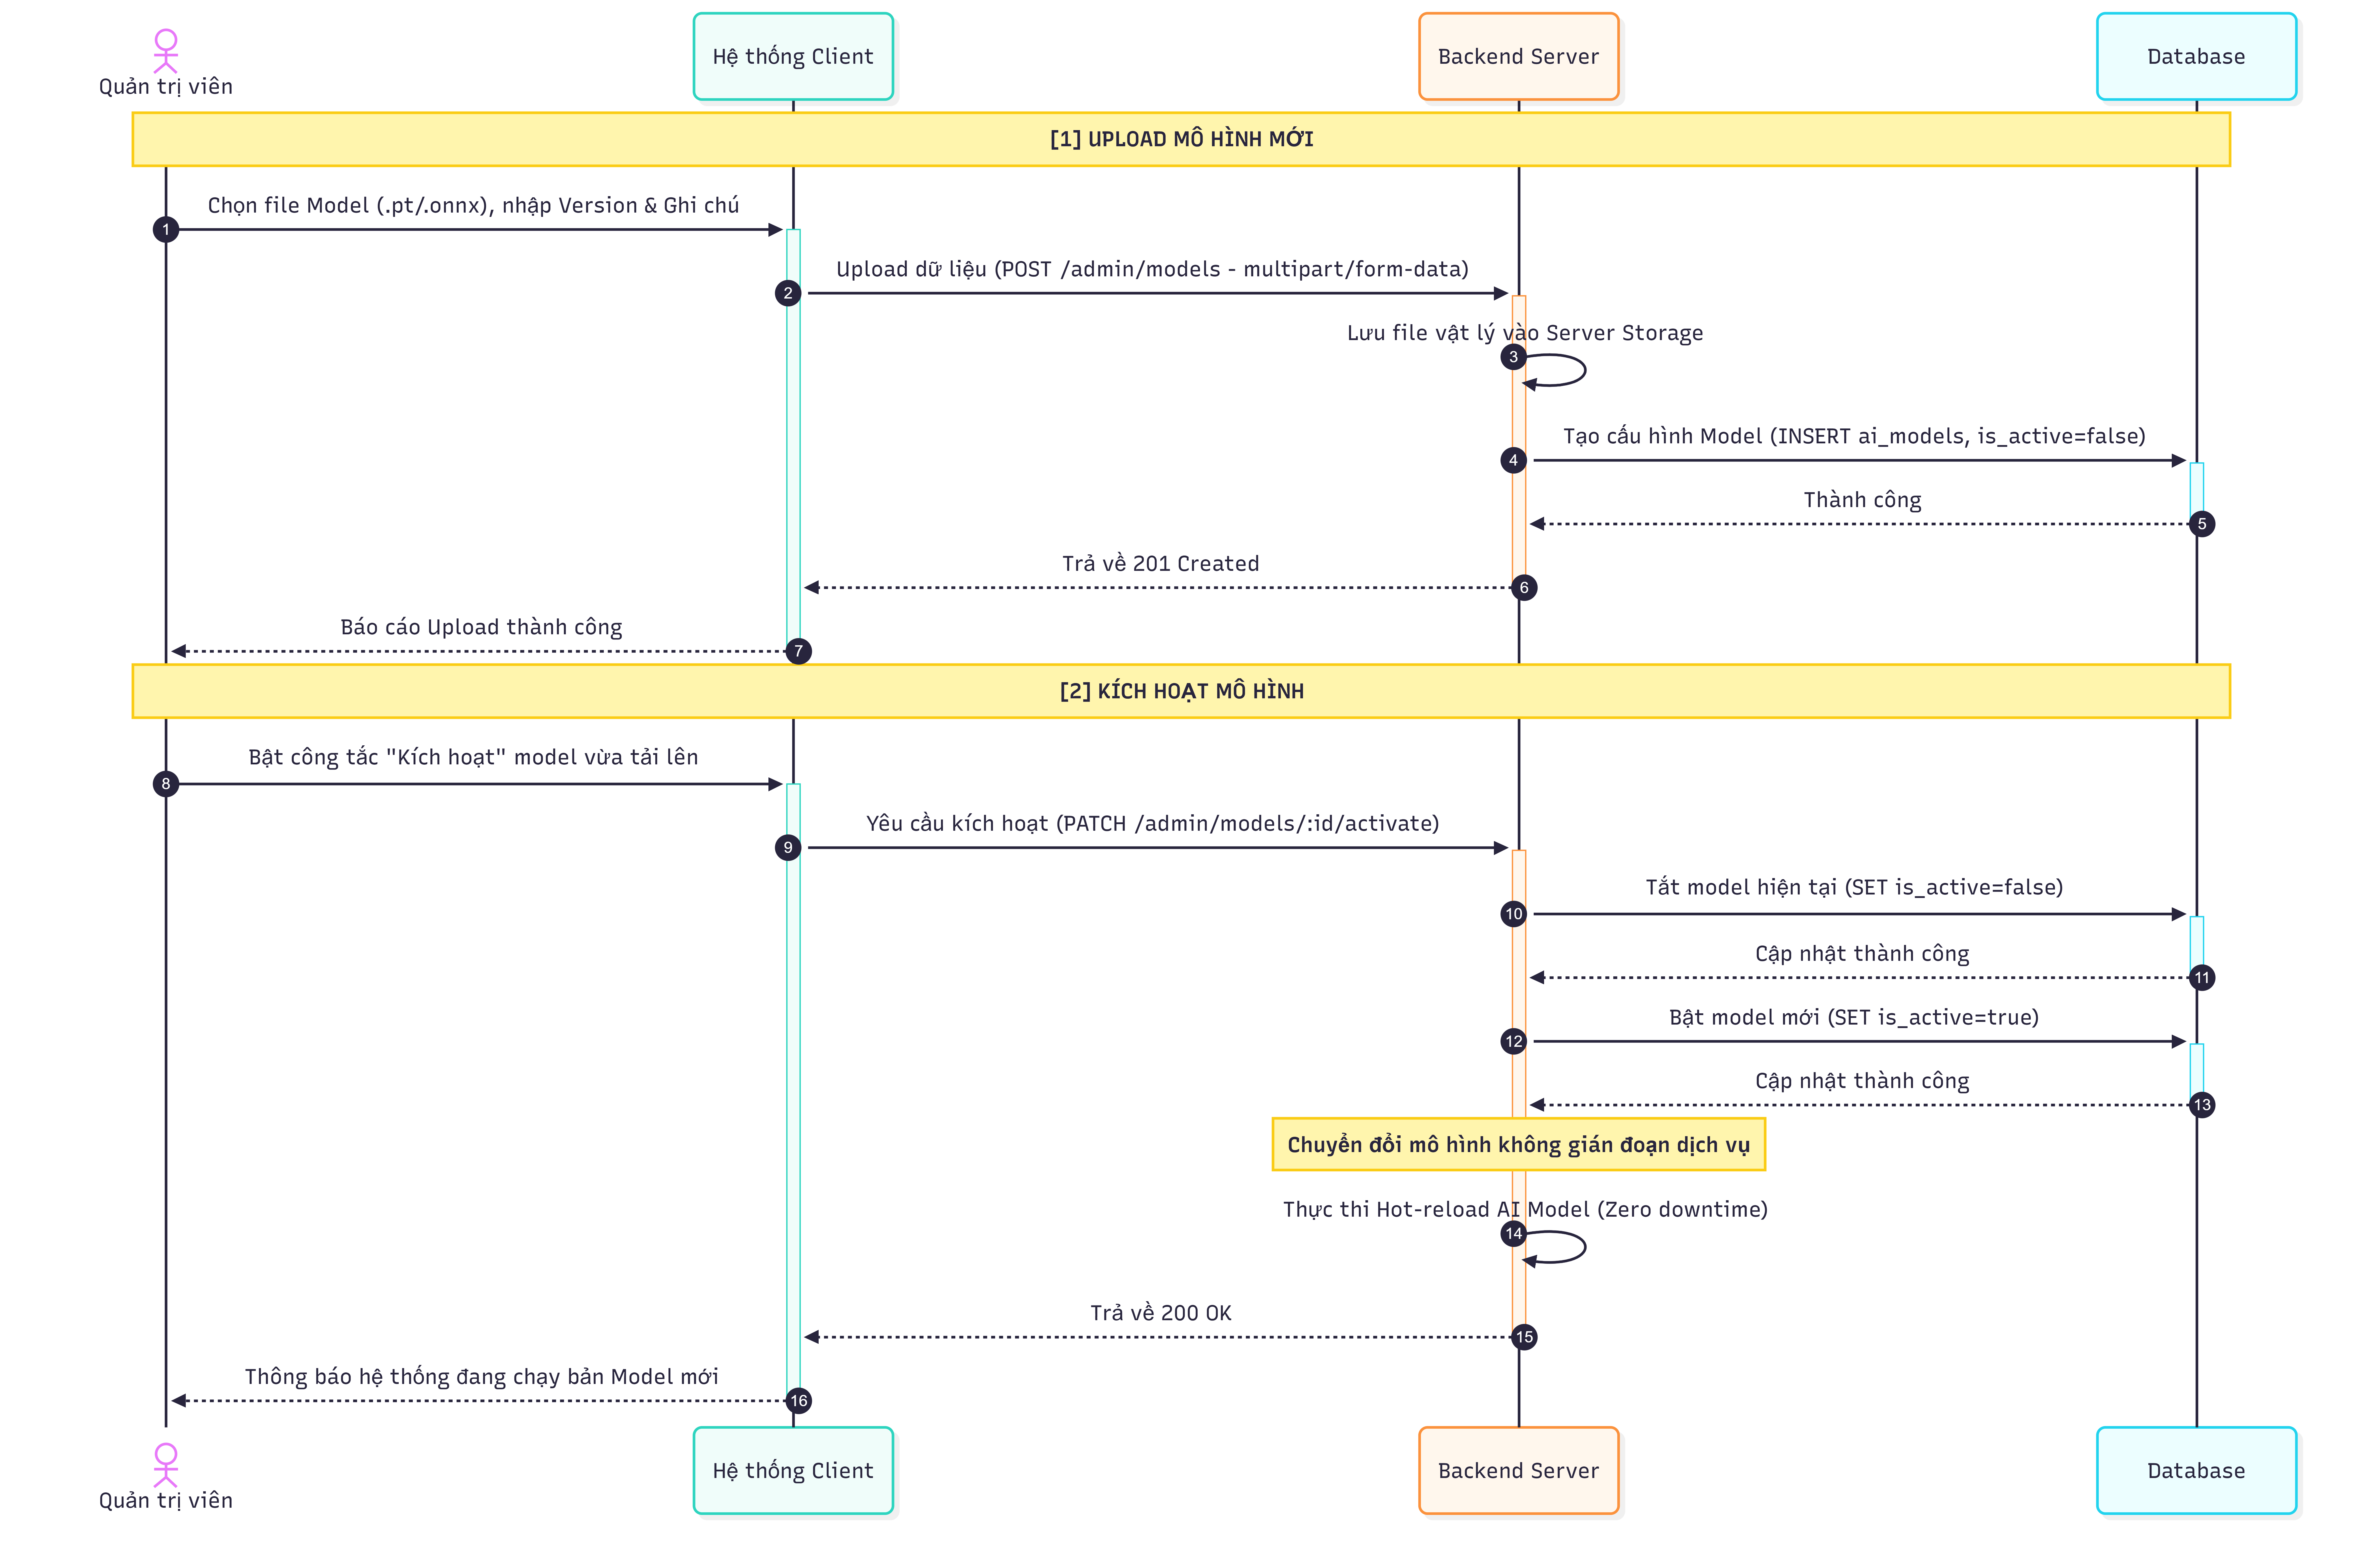
\includegraphics[width=\textwidth,height=0.85\textheight,keepaspectratio]{sd-14-model-update.png}
    \caption{Biểu đồ tuần tự: Cập nhật mô hình AI}
    \label{fig:sd-14}
\end{figure}

\subsection{SD-15: Thống kê \& Báo cáo}
% \noindent\textit{[Chèn ảnh SD-15 tại đây]}
\begin{figure}[htbp]
    \centering
    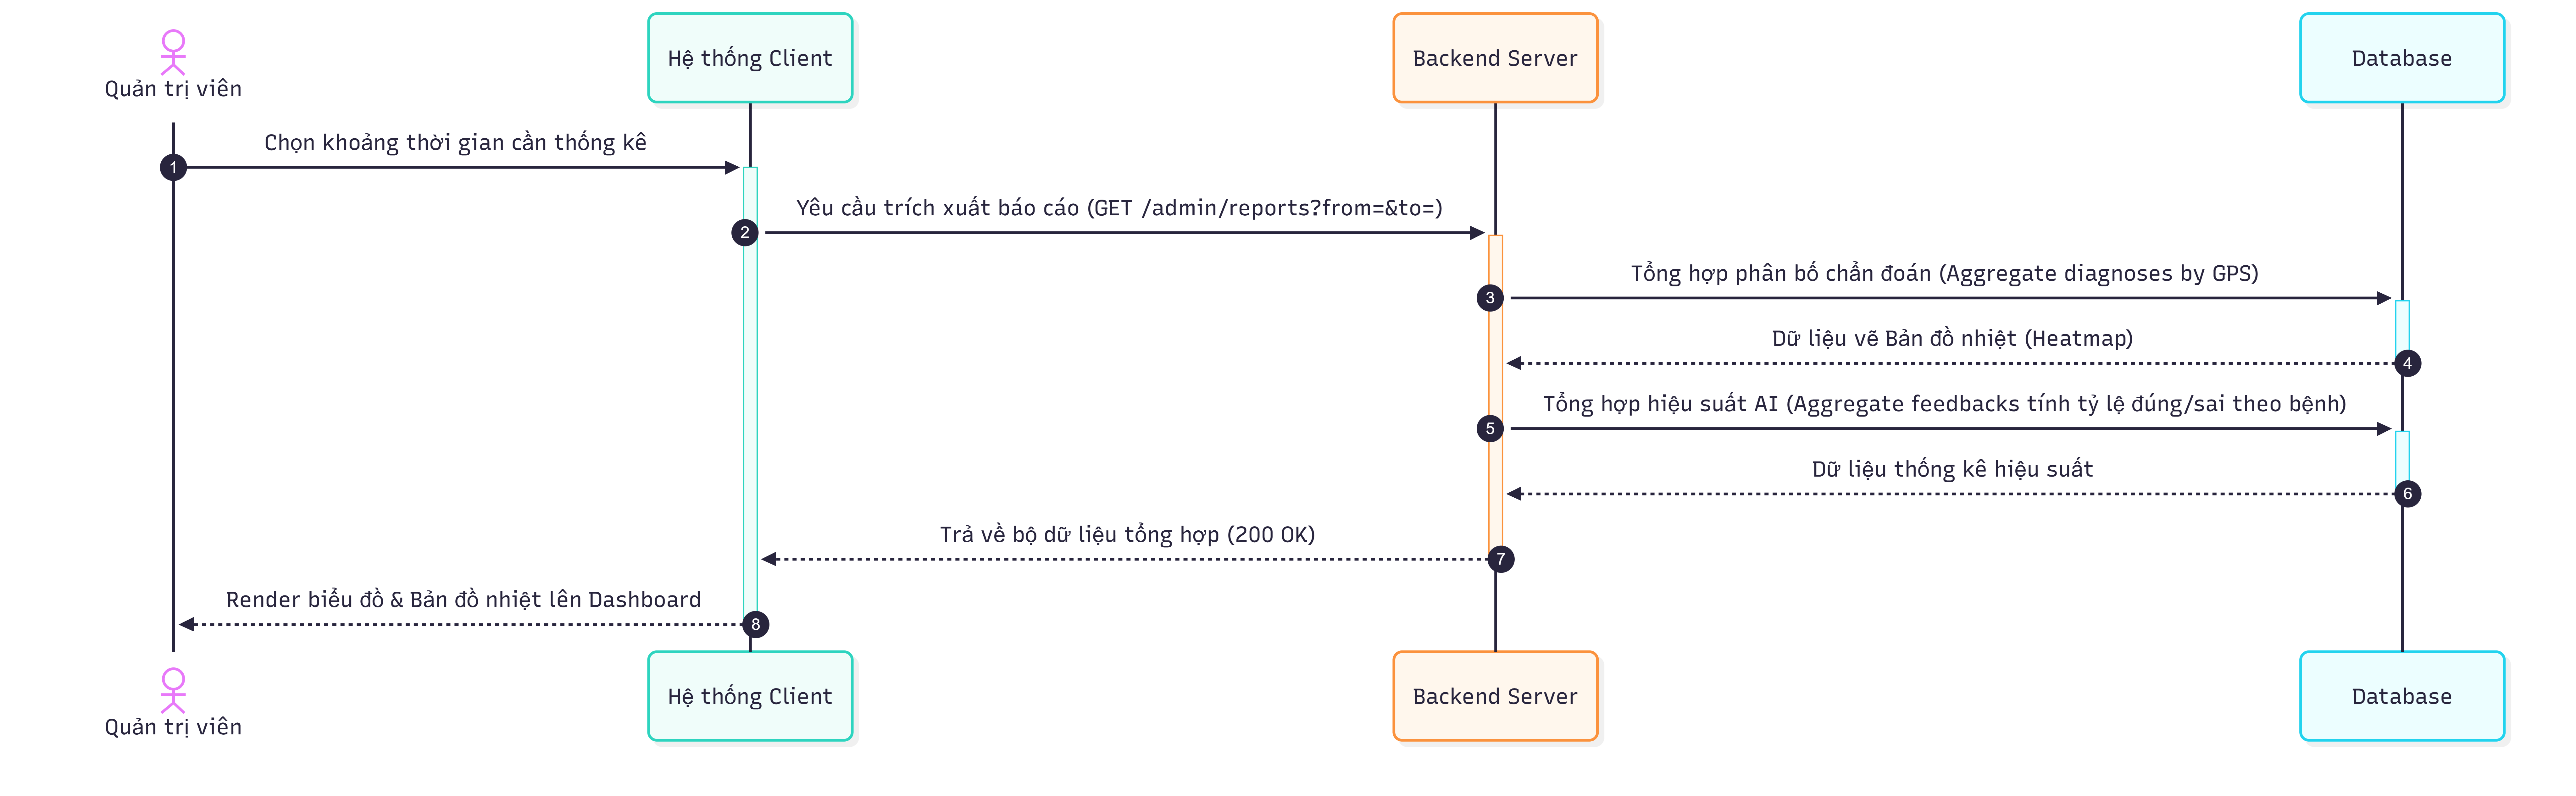
\includegraphics[width=\textwidth,height=0.85\textheight,keepaspectratio]{sd-15-reports.png}
    \caption{Biểu đồ tuần tự: Thống kê và báo cáo}
    \label{fig:sd-15}
\end{figure}

\hrulefill

% ============================================================
\section{Thiết kế Cơ sở dữ liệu}

\subsection{Bảng users}
\begin{longtable}{|l|l|l|p{5cm}|}
    \caption{Cấu trúc bảng users}                                                          \\
    \hline
    \rowcolor{headerblue}
    \textbf{Trường} & \textbf{Kiểu} & \textbf{Ràng buộc}                & \textbf{Ghi chú} \\
    \hline
    id              & UUID          & PK                                &                  \\
    \hline
    username        & VARCHAR(50)   & UNIQUE, NOT NULL                  &                  \\
    \hline
    email           & VARCHAR(255)  & UNIQUE, NOT NULL                  &                  \\
    \hline
    password        & VARCHAR       &                                   & Nullable cho Social Login \\
    \hline
    role            & ENUM          & 'user', 'admin'                   &                  \\
    \hline
    status          & ENUM          & 'active', 'inactive', 'suspended' &                  \\
    \hline
    metadata        & JSONB         &                                   & Cấu hình/thông tin bổ sung \\
    \hline
    created\_at     & TIMESTAMP     & Default now()                     &                  \\
    \hline
    updated\_at     & TIMESTAMP     &                                   &                  \\
    \hline
    \rowcolor{headerblue}
    \textbf{Indexes} & \multicolumn{3}{l|}{username, email}                                \\
    \hline
\end{longtable}

\textit{Lưu ý:} Số lần đăng nhập sai và thời gian khóa tạm thời được lưu trên \textbf{Redis}, không lưu trong CSDL.

\subsection{Bảng user\_profiles}
\begin{longtable}{|l|l|l|p{5.5cm}|}
    \caption{Cấu trúc bảng user\_profiles}                                             \\
    \hline
    \rowcolor{headerblue}
    \textbf{Trường} & \textbf{Kiểu} & \textbf{Ràng buộc}             & \textbf{Ghi chú} \\
    \hline
    id              & UUID          & PK                             &                  \\
    \hline
    user\_id        & FK            & $\rightarrow$ users.id, UNIQUE & Quan hệ 1--1     \\
    \hline
    first\_name     & VARCHAR       &                                & Họ               \\
    \hline
    last\_name      & VARCHAR       &                                & Tên              \\
    \hline
    created\_at     & TIMESTAMP     & Default now()                  &                  \\
    \hline
    updated\_at     & TIMESTAMP     &                                &                  \\
    \hline
    \rowcolor{headerblue}
    \textbf{Indexes} & \multicolumn{3}{l|}{user\_id (Unique FK)}                            \\
    \hline
\end{longtable}

\subsection{Bảng user\_social\_accounts}
\begin{longtable}{|l|l|l|p{5.5cm}|}
    \caption{Cấu trúc bảng user\_social\_accounts}                                                      \\
    \hline
    \rowcolor{headerblue}
    \textbf{Trường}     & \textbf{Kiểu} & \textbf{Ràng buộc}           & \textbf{Ghi chú}        \\
    \hline
    id                  & UUID          & PK                           &                         \\
    \hline
    user\_id            & FK            & $\rightarrow$ users.id       & Quan hệ 1--N            \\
    \hline
    provider            & VARCHAR       & NOT NULL                     & Google, Facebook, v.v.   \\
    \hline
    provider\_user\_id  & VARCHAR       & UNIQUE, NOT NULL             & ID từ nhà cung cấp      \\
    \hline
    created\_at         & TIMESTAMP     & Default now()                &                         \\
    \hline
    updated\_at         & TIMESTAMP     &                              &                         \\
    \hline
    \rowcolor{headerblue}
    \textbf{Indexes}    & \multicolumn{3}{l|}{user\_id, provider, provider\_user\_id, (user\_id, provider)} \\
    \hline
\end{longtable}

\subsection{Bảng diseases}
\begin{longtable}{|l|l|l|p{5.5cm}|}
    \caption{Cấu trúc bảng diseases}                                          \\
    \hline
    \rowcolor{headerblue}
    \textbf{Trường}  & \textbf{Kiểu} & \textbf{Ràng buộc}  & \textbf{Ghi chú} \\
    \hline
    id               & UUID          & PK                  &                  \\
    \hline
    name             & NVARCHAR(100) & UNIQUE, NOT NULL    & Tên tiếng Việt   \\
    \hline
    scientific\_name & VARCHAR(150)  & UNIQUE              & Tên khoa học     \\
    \hline
    signs            & TEXT          &                     & Dấu hiệu bệnh    \\
    \hline
    status           & ENUM          & 'visible', 'hidden' &                  \\
    \hline
    created\_at      & TIMESTAMP     & Default now()       &                  \\
    \hline
    updated\_at      & TIMESTAMP     &                     &                  \\
    \hline
    \rowcolor{headerblue}
    \textbf{Indexes} & \multicolumn{3}{l|}{name, scientific\_name}               \\
    \hline
\end{longtable}

\subsection{Bảng nutritions (Vector Database)}
\begin{longtable}{|l|l|l|p{5.5cm}|}
    \caption{Cấu trúc bảng nutritions}                                                         \\
    \hline
    \rowcolor{headerblue}
    \textbf{Trường} & \textbf{Kiểu} & \textbf{Ràng buộc} & \textbf{Ghi chú}                    \\
    \hline
    id              & UUID          & PK                 &                                     \\
    \hline
    content         & TEXT          & NOT NULL           & Nội dung tri thức                   \\
    \hline
    source          & NVARCHAR(100) &                    & Nguồn tài liệu                      \\
    \hline
    embedding       & VECTOR(1536)  &                    & Vector ngữ nghĩa (pgvector)         \\
    \hline
    chunk\_metadata & JSONB         &                    & Thông tin bổ sung, hỗ trợ GIN Index \\
    \hline
    created\_at     & TIMESTAMP     & Default now()      &                                     \\
    \hline
    updated\_at     & TIMESTAMP     &                    &                                     \\
    \hline
    \rowcolor{headerblue}
    \textbf{Indexes} & \multicolumn{3}{l|}{id (PK)}                                         \\
    \hline
\end{longtable}

\subsection{Bảng diagnoses}
\begin{longtable}{|l|l|l|p{5.5cm}|}
    \caption{Cấu trúc bảng diagnoses}                                                             \\
    \hline
    \rowcolor{headerblue}
    \textbf{Trường}      & \textbf{Kiểu} & \textbf{Ràng buộc}          & \textbf{Ghi chú}         \\
    \hline
    id                   & UUID          & PK                          &                          \\
    \hline
    user\_id             & FK            & $\rightarrow$ users.id      &                          \\
    \hline
    original\_image\_url & VARCHAR(512)  & NOT NULL                    &                          \\
    \hline
    result\_image\_url   & VARCHAR(512)  &                             &                          \\
    \hline
    gps\_lat             & DECIMAL(10,8) &                             & Tọa độ gọi API thời tiết \\
    \hline
    gps\_lng             & DECIMAL(11,8) &                             &                          \\
    \hline
    province             & TEXT          &                             & Tỉnh/thành phố           \\
    \hline
    weather\_data        & JSONB         &                             & Dữ liệu thời tiết từ API \\
    \hline
    env\_description     & TEXT          &                             &                          \\
    \hline
    model\_version\_id   & FK            & $\rightarrow$ ai\_models.id &                          \\
    \hline
    created\_at          & TIMESTAMP     & Default now()               &                          \\
    \hline
    updated\_at          & TIMESTAMP     &                             &                          \\
    \hline
    \rowcolor{headerblue}
    \textbf{Indexes}     & \multicolumn{3}{l|}{user\_id, model\_version\_id}                        \\
    \hline
\end{longtable}

\subsection{Bảng diagnosis\_results (1--N)}
\begin{longtable}{|l|l|l|p{5.5cm}|}
    \caption{Cấu trúc bảng diagnosis\_results}                                                \\
    \hline
    \rowcolor{headerblue}
    \textbf{Trường} & \textbf{Kiểu} & \textbf{Ràng buộc}         & \textbf{Ghi chú}           \\
    \hline
    id              & UUID          & PK                         &                            \\
    \hline
    diagnosis\_id   & FK            & $\rightarrow$ diagnoses.id &                            \\
    \hline
    disease\_id     & FK            & $\rightarrow$ diseases.id  &                            \\
    \hline
    confidence      & DECIMAL(5,2)  & 0--100.00                  & \% độ tin cậy              \\
    \hline
    mask\_polygon   & JSONB         &                            & Tọa độ polygon             \\
    \hline
    color           & VARCHAR(20)   &                            & Màu sắc bounding box       \\
    \hline
    advisory        & JSONB         &                            & Khuyến nghị xử lý          \\
    \hline
    created\_at     & TIMESTAMP     & Default now()              &                            \\
    \hline
    updated\_at     & TIMESTAMP     &                            &                            \\
    \hline
    \rowcolor{headerblue}
    \textbf{Indexes} & \multicolumn{3}{l|}{diagnosis\_id, disease\_id}                          \\
    \hline
\end{longtable}

\subsection{Bảng feedbacks}
\clearpage
\begin{table}[htbp]
    \centering
    \small
    \renewcommand{\arraystretch}{0.95}
    \setlength{\tabcolsep}{5pt}
    \caption{Cấu trúc bảng feedbacks}
    \begin{tabular}{|l|l|l|p{5.5cm}|}
        \hline
        \rowcolor{headerblue}
        \textbf{Trường} & \textbf{Kiểu} & \textbf{Ràng buộc}                & \textbf{Ghi chú}       \\
        \hline
        id              & UUID          & PK                                &                        \\
        \hline
        diagnosis\_id   & FK            & $\rightarrow$ diagnoses.id        &                        \\
        \hline
        user\_id        & FK            & $\rightarrow$ users.id            & Người gửi              \\
        \hline
        user\_message   & TEXT          &                                   & Lời nhắn nông dân      \\
        \hline
        status          & ENUM          & 'pending', 'accepted', 'rejected' &                        \\
        \hline
        admin\_id       & FK            & $\rightarrow$ users.id, nullable  & Admin xử lý            \\
        \hline
        admin\_response & TEXT          &                                   & Lời nhắn admin gửi lại \\
        \hline
        processed\_at   & TIMESTAMP     &                                   &                        \\
        \hline
        created\_at     & TIMESTAMP     & Default now()                     &                        \\
        \hline
        updated\_at     & TIMESTAMP     &                                   &                        \\
        \hline
        \rowcolor{headerblue}
        \textbf{Indexes} & \multicolumn{3}{l|}{diagnosis\_id, user\_id, status}                      \\
        \hline
    \end{tabular}
\end{table}

\subsection{Bảng feedback\_actual\_diseases (Junction)}
\begin{longtable}{|l|l|l|p{5.5cm}|}
    \caption{Cấu trúc bảng feedback\_actual\_diseases}                                \\
    \hline
    \rowcolor{headerblue}
    \textbf{Trường} & \textbf{Kiểu} & \textbf{Ràng buộc} & \textbf{Ghi chú}           \\
    \hline
    feedback\_id    & UUID          & PK, FK             & $\rightarrow$ feedbacks.id \\
    \hline
    disease\_id     & UUID          & PK, FK             & $\rightarrow$ diseases.id  \\
    \hline
    created\_at     & TIMESTAMP     & Default now()      &                            \\
    \hline
    updated\_at     & TIMESTAMP     &                    &                            \\
    \hline
    \rowcolor{headerblue}
    \textbf{Indexes} & \multicolumn{3}{l|}{(feedback\_id, disease\_id) [PK]}          \\
    \hline
\end{longtable}

\subsection{Bảng ai\_models}
\begin{longtable}{|l|l|l|p{5.5cm}|}
    \caption{Cấu trúc bảng ai\_models}                                          \\
    \hline
    \rowcolor{headerblue}
    \textbf{Trường} & \textbf{Kiểu} & \textbf{Ràng buộc}     & \textbf{Ghi chú} \\
    \hline
    id              & UUID          & PK                     &                  \\
    \hline
    version\_name   & NVARCHAR(50)  & NOT NULL               & Tên phiên bản    \\
    \hline
    file\_path      & VARCHAR(512)  & NOT NULL               & Đường dẫn file   \\
    \hline
    release\_notes  & TEXT          &                        & Ghi chú thay đổi \\
    \hline
    is\_active      & BOOLEAN       & Default false          & Chỉ 1 active     \\
    \hline
    uploaded\_by    & FK            & $\rightarrow$ users.id & Admin upload     \\
    \hline
    created\_at     & TIMESTAMP     & Default now()          &                  \\
    \hline
    updated\_at     & TIMESTAMP     &                        &                  \\
    \hline
    \rowcolor{headerblue}
    \textbf{Indexes} & \multicolumn{3}{l|}{id (PK)}                                \\
    \hline
\end{longtable}

\subsection{Redis Keys}
\begin{longtable}{|l|p{7.5cm}|l|}
    \caption{Các pattern key trong Redis}                                              \\
    \hline
    \rowcolor{headerblue}
    \textbf{Key Pattern}    & \textbf{Mô tả}        & \textbf{TTL}                     \\
    \hline
    login:fail:\{username\} & Số lần đăng nhập sai  & 15 phút (user) / 30 phút (admin) \\
    \hline
    otp:\{email\}           & OTP 6 số + số lần thử & 10 phút                          \\
    \hline
    verify:\{token\}        & Token xác thực email  & 24 giờ                           \\
    \hline
\end{longtable}

\subsection{Sơ đồ quan hệ thực thể (ERD)}

% \noindent\textit{[Chèn ảnh ER Diagram tại đây --- sinh từ db.dbml]}
\begin{figure}[htbp]
    \centering
    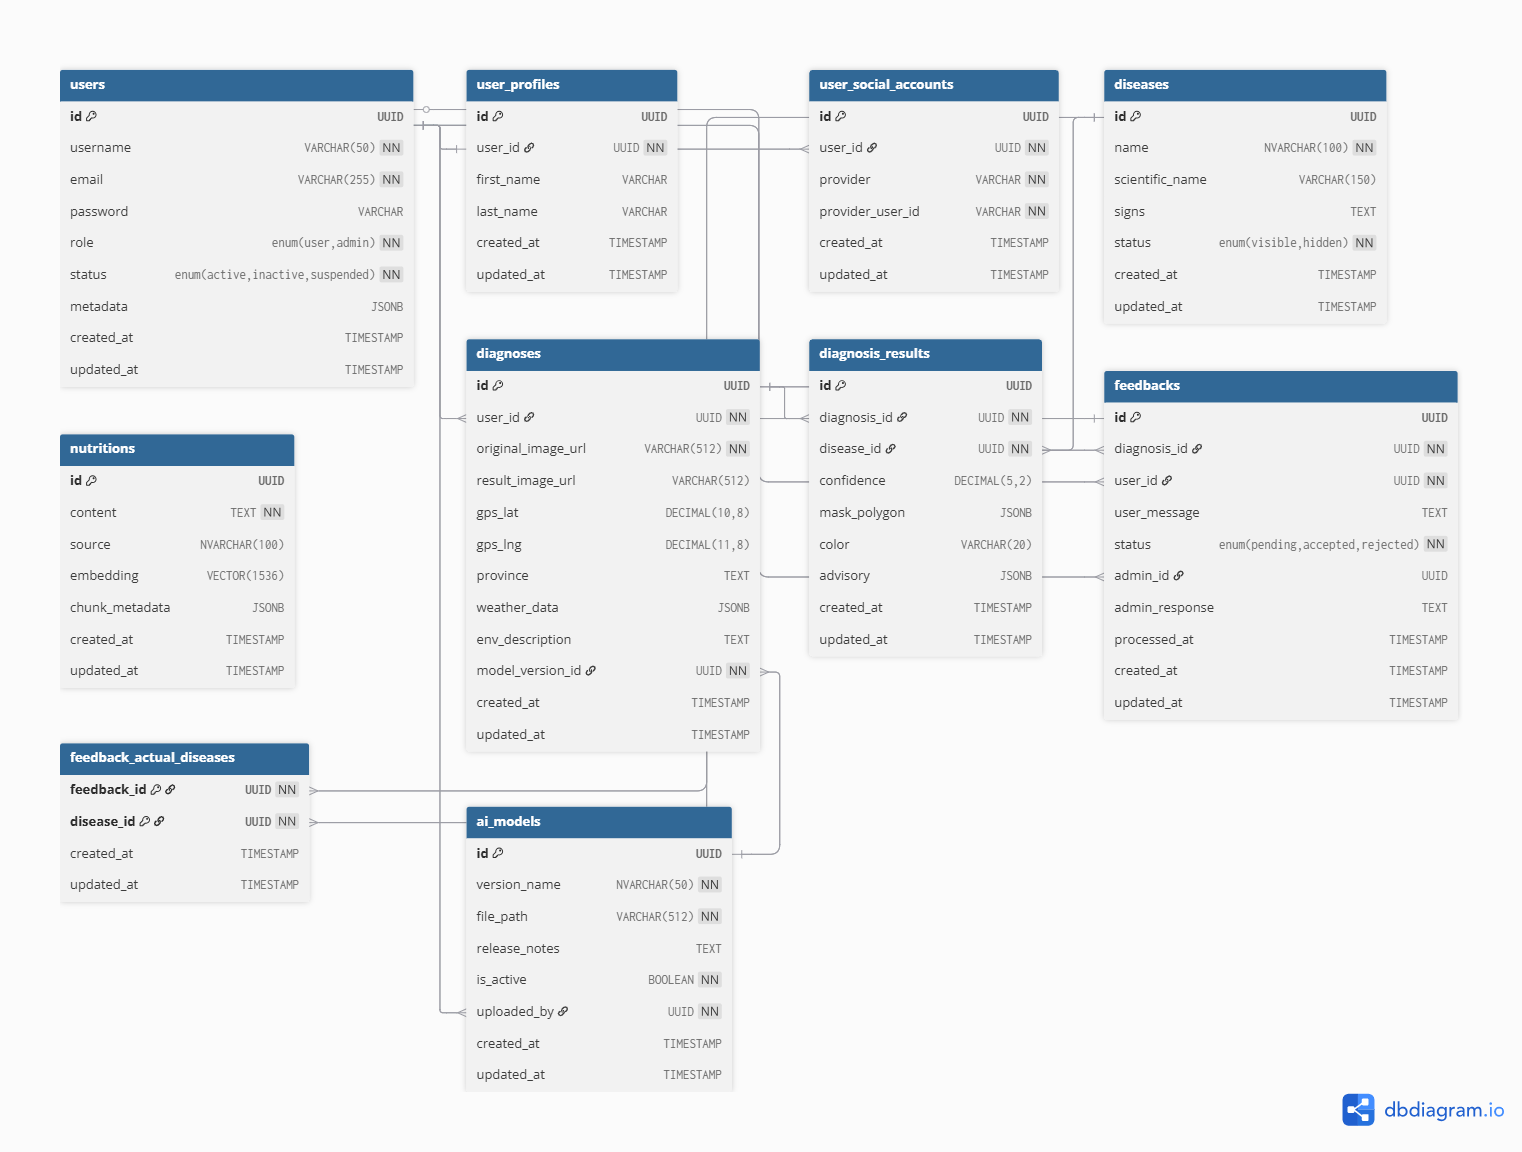
\includegraphics[width=\textwidth,height=0.85\textheight,keepaspectratio]{erd.png}
    \caption{Sơ đồ quan hệ thực thể (ERD)}
    \label{fig:erd}
\end{figure}

\hrulefill

% ============================================================
\section{Giải thích thuật ngữ}

\begin{longtable}{|l|p{11.5cm}|}
    \caption{Giải thích các thuật ngữ chuyên ngành}                                                           \\
    \hline
    \rowcolor{headerblue}
    \textbf{Thuật ngữ}    & \textbf{Giải thích}                                                               \\
    \hline
    CNN                   & Mạng nơ-ron tích chập --- thuật toán AI chuyên phân tích hình ảnh.                \\
    \hline
    Instance Segmentation & Kỹ thuật AI khoanh vùng chính xác từng đối tượng bệnh trên ảnh (pixel-level).     \\
    \hline
    pgvector              & Phần mở rộng của PostgreSQL cho phép tìm kiếm ngữ nghĩa trên dữ liệu văn bản.     \\
    \hline
    Embedding             & Biểu diễn số của văn bản để máy hiểu nghĩa, phục vụ tìm kiếm thông minh.          \\
    \hline
    RAG                   & Retrieval-Augmented Generation --- truy xuất tri thức để AI tư vấn chính xác hơn. \\
    \hline
    Redis                 & Bộ nhớ đệm tốc độ cao, dùng lưu tạm OTP và đếm lần đăng nhập sai.                 \\
    \hline
    JWT                   & Mã thông báo xác thực, giữ trạng thái đăng nhập của người dùng.                   \\
    \hline
    Bcrypt                & Thuật toán mã hóa mật khẩu một chiều, không thể giải ngược.                       \\
    \hline
    OTP                   & Mã xác thực dùng một lần, gửi qua email, hết hạn sau 10 phút.                     \\
    \hline
    GPS                   & Hệ thống định vị toàn cầu, xác định tọa độ vị trí người dùng.                     \\
    \hline
    Hot-swap              & Thay thế mô hình AI mà không cần tắt hệ thống.                                    \\
    \hline
    ERD                   & Sơ đồ thực thể quan hệ --- mô tả cấu trúc và quan hệ giữa các bảng dữ liệu.       \\
    \hline
    mask\_polygon         & Mảng tọa độ đa giác mô tả đường viền vùng bệnh trên ảnh.                          \\
    \hline
\end{longtable}

\end{document}
